% \maketitle
% \clearpage
% \tableofcontents
% \clearpage

\chapter{Introduzione}

Il cloud computing consiste in una serie di servizi che permettono di creare e gestire risorse IT on-demand con una tariffa basata sul consumo. I principali vantaggi sono la flessibilità dell'infrastruttura e la notevole riduzione dei costi di manutenzione, considerando anche che rispetto ad un'infrastruttura on-premises non c'è nessun tipo di hardware da gestire. Per questi motivi negli ultimi anni la richiesta di servizi di cloud computing è aumentata notevolmente e ad oggi di tratta di un mercato da centinaia di miliardi di dollari all'anno che vede come player principali Amazon Web Services, Google Cloud Platform e Microsoft Azure.

Purtroppo però non è tutto oro quel che luccica; esistono infatti diversi svantaggi nell'utilizzare questi tipi di servizi tra i quali il più rilevante è sicuramente il costo. Nonostante i benefici citati prima può essere poco conveniente utilizzare servizi di cloud compunting per casi d'uso in cui si ha bisogno di ingenti risorse di calcolo o di elevati volumi di storage. Per questo motivo molte realtà aziendali preferiscono creare un'infrastruttura cloud privata. Ci sono numerose piattaforme che permettono di realizzare questo tipo di infrastrutture e una di queste è OpenStack.

OpenStack è una piattaforma di cloud computing open source che permette di realizzare infrastrutture cloud sia private che pubbliche. Esistono infatti cloud provider che utilizzano OpenStack come base per erogare i loro servizi; un esempio è OVH, uno dei più grandi provider d'Europa.
OpenStack è anche scelto da molte aziende come base per il loro cloud privato per via della sua architettura modulare e grazie al fatto che le funzionalità offerte sono molto simili a quelle dei cloud provider.

\section{Il progetto}

L'obiettivo di questo progetto di tesi è prima di tutto installare e configurare un cloud privato basato su OpenStack per poi scoprirne le caratteristiche e studiarne le funzionalità nel dettaglio.

È inoltre previsto lo studio di Terraform, un Infrastructure as Code (IaC) tool, ovvero uno strumento che permette di definire infrastrutture cloud utilizzando solamente codice scritto all'interno di file di configurazione. In particolare si vuole studiare come questo strumento si integra con OpenStack e di come è possibile creare risorse all'interno di OpenStack utilizzandolo.

\section{Struttura del documento}

In questa sezione verrà esplicitata la struttura del documento descrivendo in maniera molto sintetica il contenuto di ciascun capitolo.

\begin{description}
    \item \textbf{Obiettivi} - Descrizione approfondita degli obbiettivi posti per lo svolgimento del progetto.
    \item \textbf{Progettazione del cluster} - Descrizione dell'architettura del cloud e approfondimento sulle scelte di progettazione e sulle motivazione di tali scelte.
    \item \textbf{Prerequisiti} - Descrizione dei componenti software necessari come supporto all'installazione di OpenStack (MAAS e Juju) e spiegazione delle procedure di installazione e configurazione di tali componenti.
    \item \textbf{OpenStack} - Descrizione della piattaforma OpenStack, dei suo componenti principali che verranno installati e dei software esterni necessari per far funzionare la piattaforma.
    \item \textbf{Installazione di OpenStack} - Descrizione delle procedure di installazione manuale e in bundle di OpenStack e spiegazione delle procedure di configurazione.
    \item \textbf{Utilizzo di OpenStack} - Istruzioni su come utilizzare al meglio un cloud OpenStack e su come sfruttarne a pieno le risorse.
    \item \textbf{Load Balancer} - Descrizione del servizio di load balancing di OpenStack, dei componenti che ne fanno parte, spiegazione delle procedure di installazione e di configurazione di tali componenti e istruzioni per l'utilizzo del load balancer.
    \item \textbf{Terraform} - Descrizione del tool Terraform, di come questo tool si integra con OpenStack e dei progetti Terraform realizzati durante lo svolgimento della tesi.
\end{description}

\newpage

\chapter{Obiettivi}

In questo capitolo verranno descritti i principali obiettivi di questo progetto di tesi. Alcuni termini e concetti verranno dati per scontati ma saranno poi approfonditi e spiegati nel dettaglio nei capitoli successivi.

Lo scopo principale è creare un cloud privato OpenStack che si avvicini il più possibile come funzionalità ad uno che potrebbe essere usato in una realtà aziendale e successivamente studiare in che modo Terraform si integra con OpenStack e quali funzionalità mette a disposizione.

\section{Progettazione del cluster}
Come prima cosa sarà necessario identificare l'hardware a disposizione e, considerato il vasto numero di componenti software da installare, realizzare un piano di deployment che sfrutti al massimo le risorse a nostra disposizione. Dato il numero limitato di macchine con architettura amd64 disponibili per questo progetto, alcuni dei servizi che lo supportano verranno installati su hardware a basso costo e con architettura diversa (verosimilmente Raspberry Pi), in modo da avere il numero maggiore di nodi dedicati esclusivamente ai servizi di OpenStack. Questo ovviamente verrà fatto dopo aver verificato che non ci siano incompatibilità per via delle diverse architetture.

\section{Installazione e configurazione dei sistemi di gestione del cloud}
Il tipo di deployment che è stato scelto comporta l'utilizzo di sistemi avanzati di gestione del cloud, il cui scopo è semplificare il provisioning delle macchine fisiche e l'installazione del cloud stesso; nello specifico, si tratta di MAAS e Juju (approfonditi nei capitoli \ref{subsec:maas} e \ref{subsec:juju}). Questi sistemi devono essere installati e configurati prima di procedere con l'installazione di OpenStack.

\section{Installazione manuale del cloud OpenStack}
Come scritto nella guida all'installazione di OpenStack \cite{openstack_installation_juju}, è consigliato fare la prima installazione manualmente, in modo da comprendere quali componenti formano il cloud e in che modo interagiscono tra loro. Per questo motivo è stato deciso di procedere in questa maniera prima utilizzare l'installazione in bundle.

\section{Installazione in bundle del cluster OpenStack}
La metodologia di deployment scelta supporta anche l'installazione in bundle: tutti i componenti con le relative relazioni vengono definiti all'interno di un file in formato YAML e Juju, leggendo questo file, si occupa di installare tutti i Charms necessari. Questo tipo di installazione è sicuramente molto efficiente in ambienti reali in cui si possono avere anche centinaia di macchine da gestire.

\section{Integrazione tra Terraform e OpenStack}
L'ultimo passo, dopo aver ottenuto un cloud OpenStack perfettamente funzionante, sarà quello di studiare il supporto di Terraform a OpenStack e di verificare quali funzionalità sono disponibili e quali non lo sono.
\newpage

\chapter{Progettazione del cloud}

All'interno di questo capitolo verranno descritte quelle che sono state le scelte di progettazione del cloud riguardanti architettura hardware, metodologie di deployment e architettura di rete e i motivi per cui sono state fatte determinate scelte.

\section{Hardware}\label{subsec:progettazione_hardware}

L'hardware utilizzato per lo svolgimento di questa tesi è descritto in \cref{tab:hardware_inventory}.

\begin{table}[H]
    \caption{Hardware utilizzato per il progetto.}
\begin{center}
        \begin{tabular}{ |c|c| }
\hline
\textbf{Oggetto} & \textbf{Quantità}\\
\hline
Raspberry Pi 4 8 GB & 2\\
PC con architettura AMD64 & 6\\
HDD 1TB & 12\\
Switch layer 2 & 1\\
            Adattatore Ethernet USB & 1\\
            Cavi ethernet & 9\\
\hline
\end{tabular}
\end{center}
    \label{tab:hardware_inventory}
\end{table}

\noindent
Nello specifico i PC con architettura AMD64 hanno un processore Intel Core i5-4460S, 8 GB di RAM e due HDD da 1 TB ciascuno.
% 
Inizialmente uno solo dei due HDD era collegato alla scheda madre (il secondo era comunque già all'interno della macchina), quindi è stato necessario aprire ciascun computer e collegare gli hard disk alla scheda madre con un cavo SATA. 
% 
Per fare questo è stato necessario scollegare il lettore CD perché tutte le schede madri delle macchine a disposizione hanno solamente due porte SATA.

Il motivo per cui è stato necessario utilizzare due HDD su ciascuna macchina è che Ceph, ovvero il servizio che fornisce lo storage, necessita di un hard disk fisico dedicato per poter funzionare e non può condividerlo con il sistema operativo.

Per quanto riguarda i Raspberry Pi invece, era previsto di utilizzarne solamente uno ma, successivamente alla scelta della metodologia di deployment (descritta nella \cref{sec:deplyoment_method}), è stato deciso di utilizzarne uno aggiuntivo su cui installare MAAS, in modo da avere una macchina in più da poter dedicare effettivamente a OpenStack.

\section{Metodologia di deployment}\label{sec:deplyoment_method}

Nel momento in cui sono iniziati i lavori per questo progetto di tesi l'ultima release di OpenStack era quella denominata \emph{Yoga} e supportava le seguenti metodologie di deployment \cite{openstack_deployment_guides}:
\begin{itemize}
    \item Charms Deployment
    \item Ansible in Docker Containers
    \item OpenStack-Ansible (con container LXC o Bare Metal)
    \item TripleO
\end{itemize}

\paragraph{Charms Deployment.}\label{sec:charms_deployment} Il Charms Deployment prevede l'utilizzo di MAAS per gestire il deployment delle macchine fisiche e di Juju per l'installazione e la gestione dei singoli componenti di OpenStack all'interno di ciascuna macchina. Il vantaggio di questo tipo di deployment è che l'installazione e la configurazione hanno un livello di automazione molto elevato e questo facilita tutto il processo di deployment. Dato che i servizi di OpenStack che vanno installati e configurati sono numerosi, i benefici di questo tipo di automazione non vanno sottovalutati.

Gli svantaggi principali di questa metodologia di deployment sono tre:
\begin{enumerate}
    \item è necessaria una conoscenza abbastanza approfondita di MAAS e Juju oltre che di OpenStack 
    \item i parametri di configurazione dei charm Juju sono limitati e in caso di problemi è difficile eseguire il debug o modificare le configurazioni
    \item MAAS e Juju richiedono ciascuno una macchina dedicata per funzionare, quindi c'è un overhead di macchine importante, soprattutto in situazione in cui si ha a disposizione una quantità di hardware limitata come in questo caso
\end{enumerate}

\noindent
Alla fine, nonostante gli svantaggi, questa è la metodologia di deployment scelta per lo svolgimento di questo progetto di tesi, e i suoi dettagli sono spiegati nella relativa documentazione \cite{openstack_charm_deployment_yoga}.


\paragraph{Ansible in Docker Containers} Questa metodologia di deployment consiste nell'utilizzare Kolla, un servizio di OpenStack, per installare ciascuno dei componenti necessari al cloud all'interno di un container Docker. È possibile sia installare tutto in una singola macchina che fare un deployment distribuito, quindi suddiviso tra più macchine; tutti i comandi necessari a installare e configurare i container vengono eseguiti attraverso un playbook Ansible. Il vantaggio di questo tipo di deployment è che è possibile dedicare tutte le macchine che si hanno a disposizione al cloud OpenStack mentre lo svantaggio principale è la maggiore difficoltà nella configurazione rispetto al Charms Deployment.
Un altro problema è che i requisiti minimi di questo tipo di deployment impongono che ciascuna macchina abbia due schede di rete; questo vincolo ha reso impossibile utilizzare questa metodologia in questo progetto perché le macchine a disposizione hanno una sola interfaccia di rete e procurarsi ulteriori schede di rete avrebbe aumentato sia costi che i tempi per la realizzazione del progetto.

\paragraph{OpenStack-Ansible} OpenStack-Ansible è molto simile a Ansible in Docker Containers come metodologia di deployment con l'unica differenza che i servizi invece che essere installati su container Docker sono installati direttamente sulla macchina fisica o su container LXC. Anche i vantaggi e gli svantaggi sono i medesimi e anche questa metodologia è stata scartata perché i requisiti minimi richiedevano due schede di rete su ciascuna macchina.

\paragraph{TripleO} TripleO è un servizio di OpenStack che mira a installare, gestire e operare un cloud utilizzando l'infrastruttura cloud proprietaria di OpenStack. 
% 
Ovviamente questo comporta dei costi visto che l'hardware viene fornito dal cloud provider a noleggio, quindi questa metodologia di deployment è stata scartata a priori senza ulteriori approfondimenti.

\section{Architettura del cloud}\label{sec:prog_cloud_architettura}

In \cref{fig:network_architecture} è descritta l'architettura del cloud. Come enunciato in precedenza l'insieme dell'hardware a disposizione è composto da due Raspberry Pi, sei computer desktop, uno switch, un adattatore ethernet USB e cavetteria varia per i collegamenti. 
% 
Tutti i Raspberry Pi e tutti i PC sonno stati collegati allo switch tramite cavo ethernet.

\begin{figure}[H]
    \centering
    % 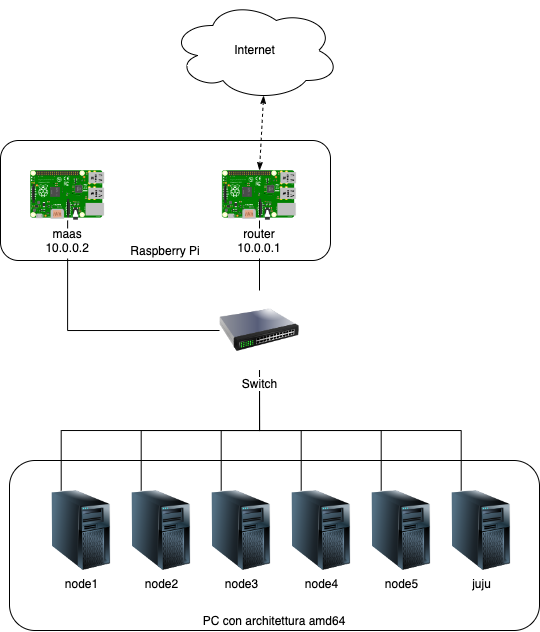
\includegraphics[scale=0.5]{tesi/files/immagini/network_architecture.png}
    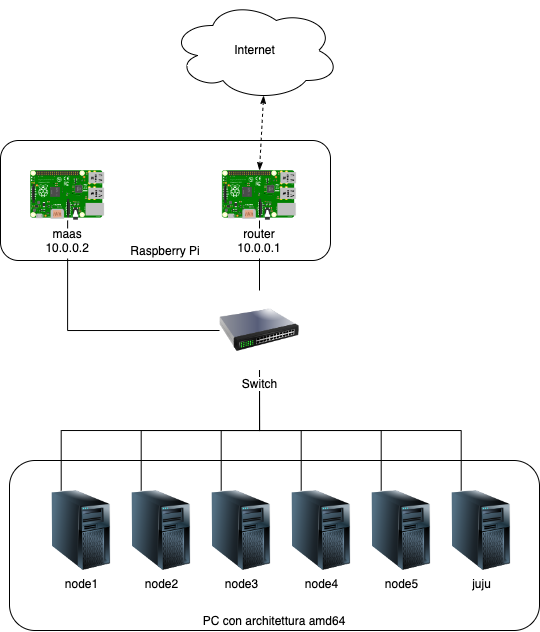
\includegraphics[width=0.8\linewidth]{tesi/files/immagini/network_architecture.png}
    \caption{Architettura di rete del cloud.}
    \label{fig:network_architecture}
\end{figure}

\noindent
Al Raspberry denominato nello schema \emph{router} è stato collegato l'adattatore ethernet USB, fornendogli un'interfaccia di rete aggiuntiva; in questo modo è stato possibile collegarlo ad internet.
% 
Il ruolo di questo Raspberry Pi è esclusivamente quello di comportarsi come un dispositivo di routing, connettendo così le due reti.
% 
La configurazione di questo dispositivo non verrà trattata in questo documento.

Il secondo Raspberry, denominato \emph{maas}, è quello su cui è stato installato l'intero sistema MAAS; la guida al deployment che è stata seguita prevedeva che MAAS fosse installato su una macchina simile a quelle utilizzate per il cloud ma, dopo un'attenta valutazione, è stato deciso di installarlo su un Raspberry Pi per avere una macchina aggiuntiva da dedicare a OpenStack.

Sul PC denominato \emph{juju} è stato installato il Juju Controller, ovvero il componente che gestisce e monitora tutti i charm che verranno installati sui nodi. 

I PC denominati \emph{nodeX} sono quelli dedicati al cloud vero e proprio, ovvero quelli su cui verranno installati tutti i componenti di OpenStack.

Inizialmente si era pensato di pianificare in quale macchina installare ciascun componente ma poi, dato che tutte le macchine sono uguali e che la guida di installazione non faceva distinzione tra le diverse macchine, si è deciso di non farlo. 
% 
Inoltre la quinta macchina è rimasta inutilizzata nel deployment iniziale ma si è rivelata fondamentale durante l'installazione del load balancer.



\subsection{Networking}\label{subsubsec:progettazione_networking}
Grazie alla modalità di deployment scelta, la configurazione della rete è molto semplice e gli indirizzi IP assegnati appartengono alla subnet \code{10.0.0.0/24}. 
% 
Come si può vedere dall'immagine in \cref{fig:network_architecture} ai Raspberry Pi \emph{router} e \emph{maas} sono stati assegnati rispettivamente gli indirizzi IP \code{10.0.0.1} e \code{10.0.0.2};
% 
le altre macchine invece non hanno indirizzi IP statici perché è il MAAS controller che si occupa di assegnarli al momento del deployment.

La scelta della subnet e degli indirizzi IP da assegnare a ciascuna macchina è totalmente arbitraria; 
% 
sono stati scelti questi perché sono gli stessi utilizzati nella guida all'installazione \cite{openstack_installation_juju}. 
% 
L'unico vincolo presente per la configurazione della rete è che almeno una delle subnet private di classe A rimanga inutilizzata; 
% 
questo perché LXD, durante l'inizializzazione automatica, sceglie tra queste subnet una da utilizzare per le proprie interfacce di rete virtuali e questa scelta viene fatta in base a quelle che non sono raggiungibili dalla macchina host \cite{lxd_init_network_error}. 
% 
Se questo vincolo non viene rispettato l'inizializzazione automatica di LXD fallisce e, anche nel caso in cui si tenti di farla manualmente, i container creati non saranno raggiungibili tramite rete.

Nelle fasi iniziale di questo progetto la rete era stata configurata sulla subnet \code{10.0.0.0/8} e questo, come si può intuire, ha causato non pochi problemi durante l'installazione dei charm su container perché l'inizializzazione di LXD stesso falliva senza dare messaggi di errore esplicativi.
% 
Il primo approccio di risoluzione è stato quello di inizializzare LXD manualmente;
% 
questo ha permesso di avviare i container contenenti i charm, ma è stato da subito chiaro che la comunicazione via rete non funzionasse correttamente.
% 
Dopo ulteriori tentativi e ricerche è stato possibile individuare il problema legato alla subnet e, dopo una riconfigurazione totale della rete, ha funzionato tutto come previsto.

\newpage

\chapter{Prerequisiti}
In questo capitolo, verranno affrontate tutte le tecnologie che si rendono necessarie per la messa in opera del cloud OpenStack.
% 
In particolare, come visto nella \cref{sec:charms_deployment}, per poter effettuare il deploy del cloud tramite \emph{Charms Deployment}, metodologia affrontata in questa sede, è necessaria l'installazione del sistema MAAS in primis e poi del sistema Juju.
% 
Di seguito verranno affrontati nei dettagli, partendo da cosa sono e dal loro funzionamento fino ad arrivare alla loro installazione e configurazione.


\section{MAAS}\label{subsec:maas}

MAAS (Metal-as-a-Service \cite{maas_home}) è uno strumento open source e gratuito di provisioning di server e di host bare-metal creato e mantenuto da Canonical.
%
Ha come compito quello di aiutare, facilitare e automatizzare l'implementazione e il provisioning dinamico su ambienti di elaborazione iperscalabili (hyperscale computing enviroments) come cloud service o big data workloads.
% 
Per fare questo, MAAS collabora con diversi servizi come Juju per coordinare applicazioni e carico di lavoro, riuscendo così a distribuire hardware e servizi che possono scalare dinamicamente verso l'alto e verso il basso.

Permette quindi il monitoraggio e il rilevamento automatico dell'infrastruttura, la creazione di cloud bare metal con server on-demand, il deploy automatizzato di immagini anche con applicazioni preinstallate, la configurazione completa della rete e dello storage e il testing e commissioning dell'hardware.



\subsection{Funzionamento: i Controller}
Il funzionamento di MAAS è suddiviso in due tipi di controller: un singolo region controller (regiond) e uno o più rack controller (rackd).
% 
Nell'esempio riportato in \cref{fig:maas_controllers} viene mostrato uno scenario dove il region controller gestisce due rack controller.

\paragraph{Region Controller.}
Il region controller è il cuore di MAAS; gestisce i rack controller fornendo loro le immagini da utilizzare per il provisioning delle macchine. Utilizza un database PostgreSQL per mantenere lo stato dei nodi registrati al sistema e ospita alcuni dei servizi di rete principali, come ad esempio il server DNS o il proxy HTTP.
%
Inoltre comunica con l'utente attraverso un'interfaccia web e una serie di API REST, dalle quali è possibile configurare e gestire tutto il sistema.

\paragraph{Rack Controller.}
 Il rack controller gestisce effettivamente le macchine collegate al sistema, occupandosi del deploy delle immagini fornite dal region controller.
 %
Gestisce la rete delle macchine, fornendo servizi come DHCP per l'assegnamento degli indirizzi IP, PXE per rendere possibile l'avvio da rete, TFTP per il trasferimento file, etc.
%
Vengono chiamati rack controller perché idealmente gestiscono individualmente singoli armadi rack con le relative macchine.
% 
Inoltre ogni rack controller è collegato via rete ad un "fabric" (vedasi la \cref{subsubsec:maas_rete} per maggior dettagli).
% 
\begin{figure}[H]
    \centering
    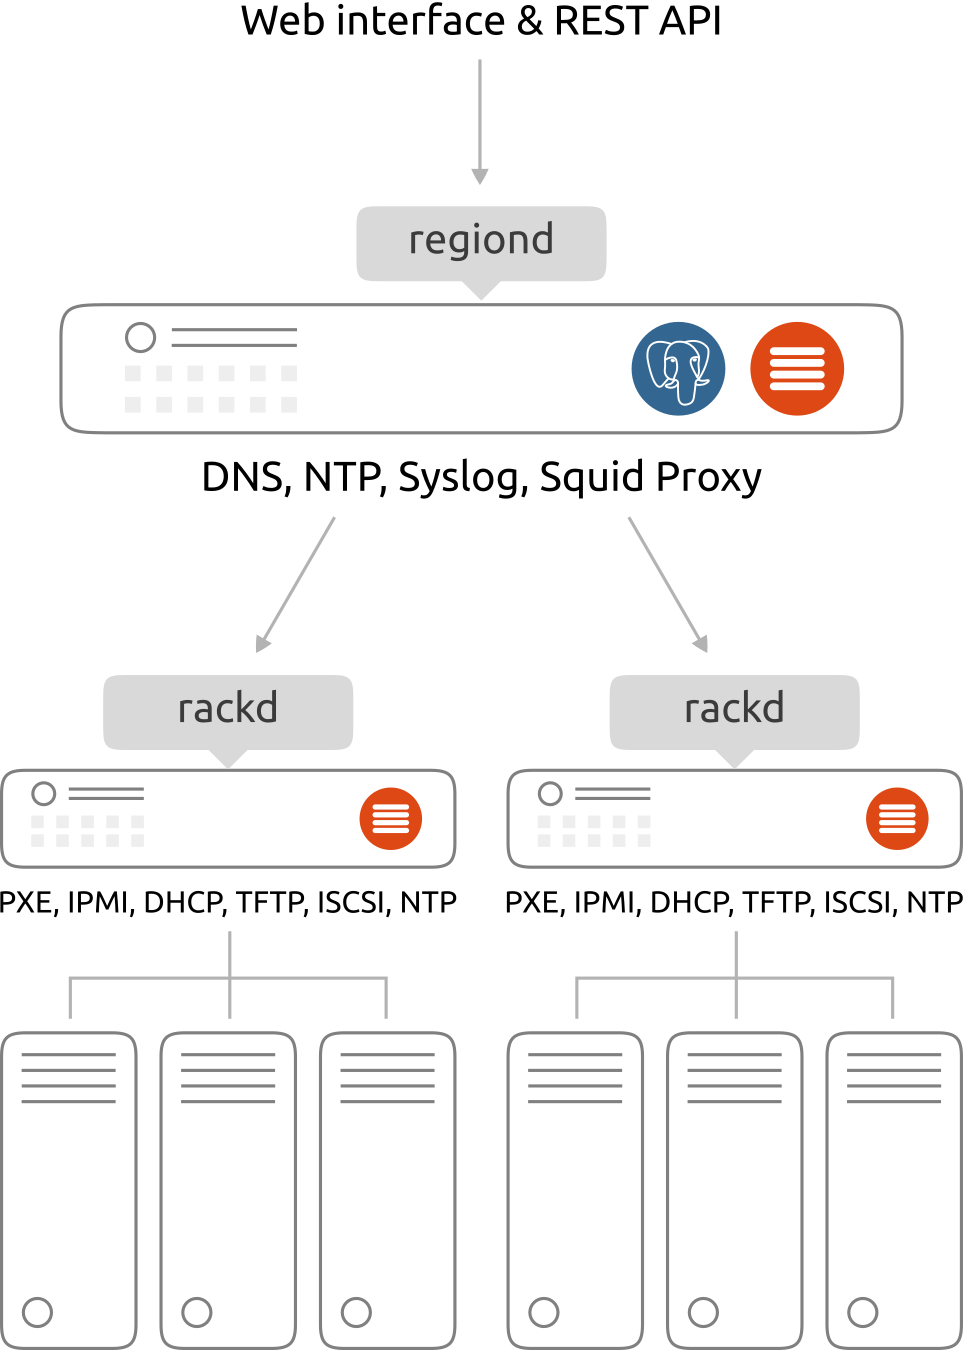
\includegraphics[width=0.45\linewidth]{tesi/files/immagini/maas/controllers}
    \caption{Configurazione con un region controller (regiond) e due rack controller (rackd) \cite{maas_how_it_works}.}
    \label{fig:maas_controllers}
\end{figure}

% \paragraph{}
% \bigskip
\noindent
Per un sistema di piccole dimensioni è possibile collocare sia il region controller che il rack controller sulla stessa macchina.\label{ref:region+rack}
%
Durante lo svolgimento di questa tesi è stato scelto questo approccio, in quanto trattasi di un piccolo scenario di prova del sistema.



\subsection{Risorse: i Nodi}\label{subsubsec:maas_node}
I nodi sono gli oggetti registrati su MAAS e ve ne sono di tre tipi:
\begin{itemize}
    \item \emph{Controllers}: sono i nodi che assumono il ruolo di region controller e rack controller.

    \item \emph{Machines}: sono i nodi che vengono gestiti tramite MAAS, ovvero quelli il cui deployment è gestito da MAAS.

    \item \emph{Devices}: sono altri dispositivi collegati alla rete che non vengono gestiti da MAAS ma che sono stati rilevati, come ad esempio router.
\end{itemize}
%
Ad ogni \textit{machine} è associata un etichetta che ne identifica lo stato attuale del lifecycle.
% 
I principali stati del lifecycle di una machine sono:
\begin{itemize}
    \item \emph{New}:
    quando una nuova risorsa viene collegata alla rete del rack controller, MAAS la rileva in automatico (fase di enlist);
    % 
    quindi l'aggiunge, registra il suo indirizzo MAC e gli associa lo stato \emph{New}.

    \item \emph{Commissioning}: è la fase durante la quale vengono raccolte e registrate le informazioni sulla configurazione dell'hardware della macchina, come quantità di RAM, numero di CPU, spazio sui dischi e altri device presenti sulla macchina stessa (e.g. GPU).

    \item \emph{Ready}: una volta terminata con successo la fase di \emph{Commissioning}, lo stato della macchina viene modificato in \emph{Ready}.

    \item \emph{Allocated}: questo stato indica che una macchina in \emph{Ready} è stata allocata ad un utente ed è pronta per il deploy.

    \item \emph{Deploying}: durante questa fase viene installato il sistema operativo in maniera completamente automatica, applicando le varie configurazioni che sono state scelte.

    \item \emph{Deployed}: è lo stato che identifica una macchina come utilizzata, ovvero con il sistema operativo installato e in funzione.

    \item \emph{Releasing}: se una macchina non è più necessaria è possibile eseguire il \textit{release}, ovvero rilasciarla in modo che possa essere riutilizzata per altri scopi. 
    % 
    Durante questa fase è possibile cancellare i dati dei dischi, scegliendo il grado di profondità dell'operazione.
    %se una macchina non è più necessaria, è possibile rilasciarla nell’insieme delle macchine Ready. 
    %
    % In questa fase è possibile cancellare i dati dei dischi, scegliendo il grado di profondità dell'operazione.
\end{itemize}
% 
Oltre a questi, esistono altri stati che permettono di identificare il malfunzionamento dei nodi o di un’azione intrapresa su di essi, come ad esempio \emph{Failed testing}, \emph{Failed Commissioning}, \emph{Failed Deployment}, \emph{Broken}, \emph{Locked}, etc.



\subsection{Gestione della rete} \label{subsubsec:maas_rete}
%
Una corretta gestione della rete di provisioning è un punto cruciale per il corretto funzionamento di MAAS.
% 
La rete viene gestita da MAAS tramite l'uso di \emph{fabric} e di \emph{space}.
% MAAS gestisce la rete tramite l'uso di \emph{fabric} e di \emph{space}.
\paragraph{Fabric.} Il fabric concettualmente corrisponde ad uno switch o ad una combinazione di switch che utilizzano il trunking (VLAN Trunking Protocol, VTP \cite{vtp}) per fornire accesso a specifiche VLAN (Virtual LAN).
%
Il fabric racchiude un insieme di VLAN, a cui appartengono le sottoreti, che possono anche essere controllate da MAAS; in questo modo si rende possibile la comunicazione tra le varie VLAN appartenenti allo stesso fabric 
% e ciò permette a MAAS di fungere anche da server DHCP.
e ciò permette a MAAS di ricoprire anche il ruolo di server DHCP.

% \sout{Infatti, per poterli gestire a pieno ha bisogno di aver completo controllo della subnet su cui sono collegate le macchine nei rack, agendo così da gateway e da server DHCP.}
In una sottorete gestita in questo modo da MAAS è possibile amministrare gli indirizzi IP sia per riservarne un pool per usi diversi dal provisioning degli host, sia per gestirli dinamicamente per usarli e associarli automaticamente durante l'enlist, commission e deploy dei nodi.
% In una sottorete gestita in questo modo da MAAS è possibile amministrare gli indirizzi IP sia riservandone un pool per allocarli per usi diversi dal provisioning degli host, sia gestirli dinamicamente per usarli e associarli automaticamente durante l'enlisting, commisisioning e deploy dei nodi.
% In una sottorete così gestita da MAAS è possibile riservare un pool di indirizzi IP ed ad allocarli per usi diversi dal provisioning degli host, mentre riservando dinamicamente gli indirizzi IP, questi vengono associati durante l'enlisting, commisisioning e deploy dei nodi.

\paragraph{Space.} 
% Uno space è un raggruppamento logico di sottoreti 
% % in base a vari parametri
% , permettendone così la comunicazione diretta tra esse.
%
Le sottoreti possono essere raggruppate tra loro anche se appartengono a fabric differenti.
% 
In questi raggruppamenti, gli space, le sottoreti possono comunicare direttamente tra loro.
% 
Ciò è utile in caso si desideri separare i nodi in base all'utilizzo o per motivi di sicurezza.
% 
Ogni space ha un indirizzo IP e una subnet mask, e i nodi assegnati ad esso possono comunicare tra loro attraverso questa rete logica.
 
Un uso comune è lo space DMZ, usato per raggruppare le sottoreti che espongono un'interfaccia web verso la rete internet pubblica; dietro questa DMZ si possono trovare ad esempio le applicazioni che non possono interagire direttamente con l'utente ma che devono invece interagire con un'interfaccia Web all'interno dello space DMZ.
% 
Inoltre, gli space facilitano l'allocazione delle macchine per Juju.

% \bigskip
\vfill\break
\vfill\break
% \newpage
\noindent
Durante l'installazione, MAAS crea un fabric di default ("fabric-0", "fabric-1", etc) per ogni subnet rilevata, mentre non crea alcuno space.
% 
Nello scenario d'esempio di questo documento
verrà utilizzata la subnet \code{10.0.0.0/24} e dunque MAAS assocerà a questa il "fabric-0", mentre non è stato creato nessuno space in quanto non si è rilevato necessario.
% verrà utilizzato un fabric denominato "fabric-0" e nessuno space.

Il diagramma in \cref{fig:maas_fabric} mostra un esempio generico di data center contenente due fabric, ognuno delle quali contiene due rack controller, diverse VLAN e uno space in comune tra i due fabric.

\begin{figure}[H]
    \centering
    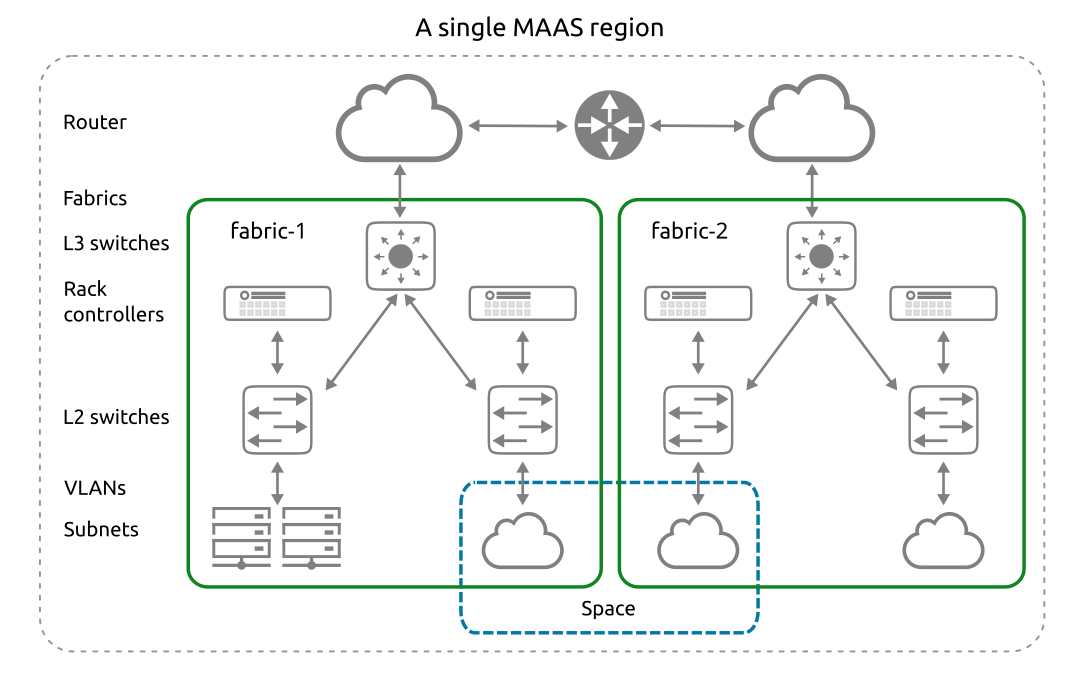
\includegraphics[width=1\linewidth]{tesi/files/immagini/maas/fabric}
    \caption{Esempio generico di configurazione di rete di un data center \cite{maas_glossary}.}
    \label{fig:maas_fabric}
\end{figure}



\subsection{Requisiti del sistema MAAS}
Il sistema che ospita MAAS non richiede un hardware eccessivamente prestante, tuttavia a seconda della configurazione finale i requisiti possono variare notevolmente.
%
Di seguito verranno mostrati due scenari d'esempio con i relativi requisiti di sistema stimati da Canonical \cite{maas_req}.


\bigskip
\paragraph{Test environment.}\label{sec:maas_req_test}
Questo è uno scenario proof-of-concept ed è l'ideale per testare e provare le potenzialità di MAAS prima di procedere con la vera e propria messa in produzione.
% 
È un tipo di scenario minimale, quindi non è necessario disporsi di macchine estremamente performanti.
% 
Nella \cref{tab:mass_requ_test} 
viene mostrata la stima delle risorse richieste da ogni componente per questo scenario.
% vengono mostrati i requisiti per un sistema di prova, con ogni componente di MAAS situato su host separati.

\begin{table}[H]
    \centering
    \caption{Risorse richieste per uno scenario proof-of-concept.}
    % \begin{adjustbox}{max width=\textwidth}
% 
% 
    \bgroup
    \def\arraystretch{1.5}% padding delle celle, 1% è default
    % 
    \begin{tabular}{||l||ccc||}
        \hhline{|t:=:t:===:t|}
        \multirow{2}{*}{}& \multicolumn{3}{c||}{TEST ENVIRONMENT} 
        \\ 
        % \cline{2-4}
        \hhline{||~||---||}
        & RAM (MB) & CPU (GHz) & DISK (GB)
        \\ 
        \hhline{|:=::===:|}
        \begin{tabular}[c]{@{}l@{}}Region controller\\(senza PostgreSQL)\end{tabular} & 512 & 0.5 & 5 
        \\ 
        \hhline{||-||---||}
        Rack controller & 512 & 0.5 & 5
        \\ 
        \hhline{||-||---||}
        PostgreSQL & 512 & 0.5 & 5
        \\ 
        \hhline{||-||---||}
        Ubuntu Server & 512 & 0.5 & 5
        \\
        \hhline{|b:=:b:===:b|}
    \end{tabular}
    % 
    \egroup
% 
% 
    % \end{adjustbox}
    \label{tab:mass_requ_test}
\end{table}

\noindent
Per questo tipo di scenario, ogni componente può essere eseguito sullo stesso host.
% 
In questo modo le risorse richieste sul singolo host diventano approssimativamente la somma delle singole specifiche: 2 GB di RAM, CPU da 2 GHz e 20 GB di spazio su disco.
% 

 

\bigskip
\paragraph{Production environment.}
Questo è il tipico scenario con cui poter approcciarsi nelle prime messe in produzione di un cloud gestito con MAAS.
% Questo è il tipico scenario che si può utilizzare per approcciarsi alla messa in produzione di un cloud gestito con MAAS.
% Questo è il tipico scenario per avviare la prima messa in produzione di un cloud gestito con MAAS.
% 

Nella \cref{tab:mass_requ_prod} 
viene mostrata la stima delle risorse richieste da ogni componente per questo scenario.
% vengono mostrati i requisiti minimi per un sistema in produzione, con ogni componente MAAS situato su host separati.
% 
%È bene evidenziare che a seconda della complessità del sistema, del numero di rack controller e dei relativi nodi collegati, del carico sul region controller e nel numero di immagini da mantenere, le risorse richieste possono aumentare.
È bene evidenziare che le risorse richieste sono influenzate da diversi fattori, tra cui: complessità del sistema, numero di rack controller, numero dei nodi collegati a ciascun rack controller, carico sul region controller e numero di immagini da mantenere.

\begin{table}[H]
    \centering
    \caption{Risorse richieste per un ipotetico scenario in produzione.}
    % \begin{adjustbox}{max width=\textwidth}
% 
% 
    \bgroup
    \def\arraystretch{1.5}% padding delle celle, 1% è default
    % 
    \begin{tabular}{||l||ccc||}
        \hhline{|t:=:t:===:t|}
        \multirow{2}{*}{}& \multicolumn{3}{c||}{PRODUCTION ENVIRONMENT} 
        \\ 
        % \cline{2-4}
        \hhline{||~||---||}
        & RAM (MB) & CPU (GHz) & DISK (GB)
        \\ 
        \hhline{|:=::===:|}
        \begin{tabular}[c]{@{}l@{}}Region controller\\(senza PostgreSQL)\end{tabular} & 2048 & 2.0 & 5 
        \\ 
        \hhline{||-||---||}
        Rack controller & 2048 & 2.0 & 20
        \\ 
        \hhline{||-||---||}
        PostgreSQL & 2048 & 2.0 & 20
        \\ 
        \hhline{||-||---||}
        Ubuntu Server & 512 & 0.5 & 5
        \\
        \hhline{|b:=:b:===:b|}
    \end{tabular}
    % 
    \egroup
% 
% 
    % \end{adjustbox}
    \label{tab:mass_requ_prod}
\end{table}

% In questa casistica, includendo PostgreSQL nel region controller, i requisiti per lo scenario del sistema in produzione diventano:

\noindent 
In questo modo è possibile creare uno scenario in produzione con le seguenti caratteristiche:

\begin{itemize}
    \item un region controller (incluso PostgreSQL) installato su un host avente 4.5 GB di RAM, CPU da 4.5 GHz e 45 GB di spazio su disco;

    \item un rack controller installato su un host avente 2.5 GB di RAM, CPU da 2.5 GHz e 40 GB di spazio su disco.
\end{itemize}

\noindent
I requisiti descritti per questo sistema non coprono le specifiche dei nodi che verranno collegati al rack controller bensì solamente all'infrastruttura MAAS.
% 
In ultimo, un rack controller non dovrebbe gestire più di 1000 nodi, indipendentemente da come sono suddivisi tra le sottoreti. 



\subsection{Installazione}\label{subsubsec:maas_install}
\paragraph{Preparazione hardware.}
Come anticipato nella \cref{subsec:progettazione_hardware}, il cloud progettato in questa tesi è costituito da:
\begin{itemize}
    \item Una macchina dedicata all'installazione completa del sistema MAAS (sia il region che il rack controller come spiegato in fondo alla sezione \ref{ref:region+rack}).
    % con accesso sia alla rete esterna che a quella interna del sistema.

    \item Una macchina dedicata al controller Juju (vedasi la \cref{subsubsec:juju_install}).
    
    \item Quattro nodi sui quali verrà effettivamente installato il cloud OpenStack più un quinto per sviluppi successivi.
\end{itemize}
% 
In questo capitolo verrà trattata la sola installazione del sistema MAAS.

\bigskip
% Dovendo il rack controller gestire un numero esiguo di macchine, non è necessario disporre di una potenza computazionale eccessivamente elevata.
% 
Date le piccole dimensioni del cloud e del sistema progettato in questa sede, e dato che il rack controller deve gestire un numero esiguo di macchine, non è necessario disporre di una potenza computazionale eccessivamente elevata.
% 
Si è quindi deciso di adottare come macchina per MAAS l'SBC Raspberry Pi 4 Model B (come spiegato nel capitolo \ref{subsec:progettazione_hardware}) con le seguenti caratteristiche:
\begin{itemize}
    \item[] 8 GB di RAM, CPU quad-core ARM64 da 1.5 GHz e 128 GB di storage su scheda micro SD (per ulteriori dettagli sulle specifiche, si veda \cite{rasp_spec}).
\end{itemize}
% 
Nonostante la frequenza della CPU sia leggermente inferiore a quella consigliata da Canonical nei vari scenari d'esempio (\cref{sec:maas_req_test}), durante tutto lo sviluppo non sono stati riscontrati né rallentamenti né altre problematiche all'interno del sistema MAAS. 


\paragraph{Preparazione software.}
Il sistema operativo installato sul Raspberry è \emph{Raspberry Pi OS} \cite{rasp_os}, basato sul sistema Debian 11 (la quale installazione in questa tesi non verrà trattata), mentre la versione di MAAS installata è la 3.1.0.
% 
Durante tutte le fasi di installazione, verrà utilizzato il package manager \emph{snap} per l'installazione e gestione del software.

L'intero sistema è situato all'interno della sottorete \code{10.0.0.0/24}, il Raspberry ospitante MAAS ha l'indirizzo IP statico \code{10.0.0.2} (vedere capitolo \ref{subsubsec:progettazione_networking} per maggiori dettagli).
%
Inoltre il sistema MAAS sarà l'unico fornitore dei servizi DHCP e DNS all'interno della rete.

\paragraph{N.B.} Rispetto ad un'installazione da manuale basata sul sistema operativo Ubuntu 20.04 con architettura AMD64, quella affrontata in questa sede differisce leggermente essendo basata sul sistema operativo Raspberry Pi OS (Debian 11) con architettura ARM64.
% 
Tutte le eventuali differenze riscontrate verranno spiegate e mostrate nei dettagli.

% \subsection*{}
\bigskip\bigskip\noindent
 Per maggior informazioni sulle seguenti fasi di installazione, fare riferimento alla guida OpenStack \cite{maas_install_openstack} e alla documentazione MAAS \cite{maas_install_doc}.


\subsection{Installazione del region e rack controller}
Durante questa fase di installazione, verranno utilizzati comandi da terminale per installare MAAS sul Raspberry.
% Questa fase d'installazione sarà basata sull'esecuzione di comandi dal terminale sulla macchina dove installare MAAS.

% workaround brutto_ dopo il primo backslash c'è uno spazio
% \paragraph{}\ \\%\noindent
\bigskip \noindent
Come prima cosa, verrà installato MAAS 3.1.0.
% 
\begin{lstlisting}[
    language=mybash, 
    caption={Installazione di MAAS.}, 
    label={lst:maas_install}
]
sudo snap install ^nf^maas^nf^ ^c^--channel=^c^3.1/stable
\end{lstlisting}
% \lstinputlisting[
%     language=mybash, 
%     caption={Installazione di MAAS.}, 
%     label={lst:maas_install},
%     firstline=1,
%     lastline=1
% ]
% {tesi/files/installazioni/per import/CLI/maas}

% \paragraph{}\ \\%\noindent
\bigskip \noindent
Successivamente verrà scaricato e configurato il database PostgreSQL che verrà utilizzato da MAAS in questo scenario.
% 
Questo passaggio è opzionale e non è da eseguire se si desidera utilizzare un database PostgreSQL esterno.
% 
\begin{lstlisting}[
    language=mybash, 
    caption={Installazione del DB PostgreSQL.}, 
    label={lst:maas_test-db_install}
]
sudo snap install maas-test-db
\end{lstlisting}
% \lstinputlisting[
%     language=mybash, 
%     caption={Installazione del DB PostgreSQL.}, 
%     label={lst:maas_test-db_install},
%     firstline=2,
%     lastline=2
% ]
% {tesi/files/installazioni/CLI/maas}
% 
% \paragraph{}\ \\%\noindent
\bigskip \noindent
Dopo aver installato MAAS, bisogna inizializzare il sistema e configurare region e rack controller.
% Una volta eseguito, non è più possibile richiamare l'init in un secondo momento.
% 
Eseguire \code{sudo mass init -{}-help} per maggiori dettagli.
% 
\begin{lstlisting}[
    language=mybash, 
    caption={Inizializzazione del region e rack controller del sistema MAAS.}, 
    label={lst:maas_init}
]
sudo maas init region+rack --maas-url http://10.0.0.2:5240/MAAS --database-uri maas-test-db:///
\end{lstlisting}
% \lstinputlisting[
%     language=mybash, 
%     caption={Inizializzazione del sistema MAAS - region e rack controller.}, 
%     label={lst:maas_init},
%     firstline=3,
%     lastline=3
% ]
% {tesi/files/installazioni/CLI/maas}
% 
\begin{itemize}
    \item Indicando al comando \code{init} il valore \code{region+rack}, viene specificato che il sistema MAAS installato avrà il ruolo sia di region controller che di rack controller.

    \item Con l'argomento \code{-{}-maas-url} viene specificato l'indirizzo URL dove è situato l'accesso per l'interfaccia utente web; essendo gestito dal region controller, va indicato il suo indirizzo IP.
    % 
    In questo caso è la stessa macchina Raspberry, avente indirizzo IP \code{10.0.0.2}.
    
    L'indirizzo IP all'interno dell'URL va quindi sostituito nel caso in cui si voglia configurare in maniera differente.

    \item Con l'argomento \code{-{}-database-uri} viene specificato l'URI del database PostgreSQL che MAAS andrà ad utilizzare;
    % 
    nel sistema installato per questo progetto viene utilizzato il database di test fornito direttamente da MAAS (\cref{lst:maas_test-db_install}), ma è possibile specificare un URI che rimanda ad un database PostgreSQL esterno nel seguente formato:\\\noindent
    % \begin{itemize}
    %     \item[]
        % \code{postgres://<user>:<password>@<host>:<port>/<database>}
        % https://www.postgresql.org/docs/current/libpq-connect.html#id-1.7.3.8.3.6
    % \end{itemize}
    {
      \code{postgresql://[user[:password]@][[host][:port]][/dbname]}\\
      \code{[?name=value[\&...]]}
    }
        
\end{itemize}

% \paragraph{}\ \\%\noindent
\bigskip
\noindent
A questo punto, verranno create le credenziali di amministratore.
% 
\begin{lstlisting}[
    language=mybash, 
    caption={Creazione delle credenziali d'amministratore.}, 
    label={lst:maas_admin}
]
sudo maas createadmin --username admin --password ubuntu --email admin@example.com --ssh-import lp:<usernameLaunchpad>
\end{lstlisting}
% \lstinputlisting[
%     language=mybash, 
%     caption={Creazione delle credenziali d'amministratore.}, 
%     label={lst:maas_admin},
%     firstline=4,
%     lastline=4
% ]
% {tesi/files/installazioni/CLI/maas}
% 
\begin{itemize}
    \item Con l'argomento \code{-{}-email} viene indicato l'indirizzo e-mail dell'account amministratore;
    % 
    tuttavia non è necessario che l'indirizzo e-mail esista veramente, in quanto in realtà non viene utilizzato da MAAS.

    \item Con l'argomento \code{-{}-ssh-import} è possibile inserire la propria chiave ssh pubblica  all'interno di MAAS importandola dal proprio profilo
    GitHub\footnote{GitHub: \url{https://github.com}, ultimo accesso 13 Gennaio 2023.} 
    o
    Launchpad\footnote{Launchpad: \url{https://launchpad.net/}, ultimo accesso 13 Gennaio 2023.}.
    % https://tex.stackexchange.com/questions/38857/labeling-a-footnotemark
    % 
    Per importare la chiave da Launchpad è necessario inserire il nome del profilo preceduto da "\code{lp:}", per GitHub va sempre inserito il nome del profilo ma questa volta preceduto da "\code{gh:}".
    % 
    Questa chiave potrà poi essere inserita all'interno dei nodi in fase di deploy e servirà per poter accedere alle singole macchine una volta che il sistema operativo verrà installato da MAAS.
    % 
    È possibile saltare questa configurazione omettendo l'argomento e gestire ulteriori chiavi da interfaccia in un secondo momento (si veda il punto \ref{itm:ssh_admin} e il paragrafo successivo nella \cref{sec:other_conf}).
\end{itemize}

% \paragraph{}\ \\%\noindent
\bigskip \noindent
In ultimo verrà copiata la chiave API dell'utente "admin" e memorizzata in un file a parte;
% 
questa servirà nei passaggi successivi per l'installazione di Juju (\cref{lst:juju_maas-creds-yaml} nella \cref{subsubsec:juju_install}).
% 
Nel caso in cui non si voglia salvare questa chiave su file, è possibile successivamente ricavarla da interfaccia web (si veda il terzo paragrafo della \cref{sec:other_conf}).
% 
\begin{lstlisting}[
    language=mybash, 
    caption={Salvataggio della chiave API.}, 
    label={lst:maas_apikey},
]
sudo maas apikey --username admin > %*$\sim$*)/admin-api-key-file
\end{lstlisting}
% \lstinputlisting[
%     language=mybash, 
%     caption={Salvataggio della chiave API.}, 
%     label={lst:maas_apikey},
%     firstline=5,
%     lastline=5
% ]
% {tesi/files/installazioni/per import/CLI/maas}

\bigskip\noindent
%In \cref{sec:appendice_maas} è possibile visionare l'elenco dei comandi precedentemente descritti in un unico raggruppamento.


\subsection{Configurazione}\label{subsubsec:maas_conf}
% 
Giunti a questo punto, è possibile accedere all'interfaccia utente web attraverso l'uso del browser.
% 
L'URL dell'interfaccia web a cui collegarsi è quello inserito nel \cref{lst:maas_init} nell'argomento \code{-{}-maas-url}, in questo caso:
% 
\begin{itemize}
    \item[]URL: \textbf{http://10.0.0.2:5240/MAAS}
\end{itemize}
% 
Le credenziali da immettere sono quelle inserite nel \cref{lst:maas_admin}, ovvero:
% 
\begin{itemize}
    \item[]Username: \textbf{admin}

    \item[]Password: \textbf{ubuntu}
\end{itemize}

% \paragraph{}\ \\%\noindent 
\bigskip \noindent
Al primo accesso verranno presentate delle schermate di benvenuto;
% 
da queste è già possibile configurare vari parametri del sistema MAAS che si andrà ad utilizzare.

In questo scenario sono state inserite le configurazioni seguenti:
% 
% \begin{itemize}
\begin{enumerate}
    \item \textbf{Region name.} Questa stringa identifica il nome del sottodominio dei nodi secondo la nomenclatura FQDN \cite{fqdn}.
    % 
    In questa sede è stato scelto \emph{oscluster.unibo.it}; ad esempio il node1 sarà identificato come \emph{node1.oscluster.unibo.it}.

    \item \textbf{DNS forwarder.} Qui vanno indicati gli indirizzi IP dei server DNS esterni che si vogliono utilizzare. Questi serviranno per risolvere i domini che non sono gestiti da MAAS.
    % 
    In questo caso sono stati utilizzati gli indirizzi \colorbox{lgray}{8.8.8.8} e \colorbox{lgray}{8.8.4.4}, ovvero i server DNS di Google.

    \item
    % \phantomsection
    \label{itm:image_ubuntu}
    \textbf{Ubuntu.} In questa sezione è possibile scegliere le immagini di Ubuntu da importare selezionandole per sorgente, versione e architettura.
    % 
    % Quando vengono selezionate, viene avviato anche il download delle stesse.
    % 
    Nel caso di questo progetto sono state scaricate dalla sorgente maas.io le immagini 20.04 LTS e 22.04 LTS per architettura AMD64 (come richiesto dalle istruzione di installazione di OpenStack).

    Una volta scaricate le immagini scelte, premere su "\emph{Continue}" per proseguire con la configurazione.

    \item
    % \phantomsection
    % \makeatletter\def\@currentlabel{Configurazione SSH}\makeatother
    \label{itm:ssh_admin}
    \textbf{SSH keys for admin.} In questa ultima sezione è possibile aggiungere varie chiavi ssh pubbliche in tre modi.
    
    I primi due, come menzionato nel \cref{lst:maas_admin}, sono attraverso le piattaforme Launchpad e GitHub;
    % 
    una volta selezionata la piattaforma dalla quale si vuole importare la chiave, va indicato lo username preceduto da \code{lp:} per Launchpad o da \code{gh:} per GitHub (per esempio \code{lp:user1} o \code{gh:user2}).
    
    Il terzo approccio invece consiste nel caricare la chiave pubblica manualmente copiandola da un file sul proprio computer e cliccando sul bottone "\emph{Import}" per salvarla.
    
    Una volta importate tutte le chiavi desiderate, premere su "\emph{Go to the Dashboard}" per terminare fase di configurazione guidata.
\end{enumerate}
% \end{itemize}

% \paragraph{}
\bigskip\phantomsection\label{sec:other_conf}\noindent
%\ \\%\noindent 
Al termine della configurazione guidata si ha libero accesso al sistema.
% 
Se si vogliono modificare o visionare le impostazioni configurate fino ad ora, basterà premere "\emph{Settings}" nel menù in alto.
% 
In "\emph{admin}" sempre nel menù in alto è possibile aggiungere ulteriori chiavi ssh e visionare la chiave API nel caso non fosse stata salvata nel \cref{lst:maas_apikey}.

% \paragraph{}\ \\
\bigskip
A questo punto è possibile aggiungere e gestire i vari nodi e procedere con il deploy delle immagini; tuttavia, prima di proseguire, è importante  configurare e abilitare il server DHCP, altrimenti MAAS non sarà in grado di amministrare correttamente i nodi.
% 
% \begin{itemize}
\begin{enumerate}\setcounter{enumi}{4}
    \item \textbf{DHCP.} Per abilitare il DHCP seguire i seguenti passaggi.
    \begin{enumerate}
        \item Premere su "\emph{Subnets}" nel menù in alto; comparirà una schermata che mostra le varie sottoreti che MAAS ha rilevato.
 
        \item Premere sulla VLAN desiderata, in genere denominata come \emph{untagged}.

        \item In questa schermata verranno mostrate le informazioni riguardanti la VLAN scelta.
        % 
        Nel menù a tendina "\emph{Take action}" premere su "\emph{Provide DHCP}" per far comparire la schermata di abilitazione del DHCP.

        \item Spuntare "\emph{MAAS provides DHCP}" e "\emph{Provide DHCP from rack controller}".
        % 
        Dopodiché, selezionare la subnet a cui riservare un pool di indirizzi IP che il DHCP andrà ad utilizzare in fase di elinst delle macchine, quindi inserire l'IP di partenza in "\emph{START IP ADDRESS}" e l'IP finale in "\emph{END IP ADDRESS}".

        \item Infine, premere su "\emph{Configure DHCP}".
    \end{enumerate}
        In questa sede, come mostrato in \cref{fig:maas_config_dhcp}, è stato scelto un pool di 14 indirizzi IP a partire dal \code{10.0.0.240} fino al \code{10.0.0.253}.
\end{enumerate}
% \end{itemize}
% 
\begin{figure}[H]
    \centering
    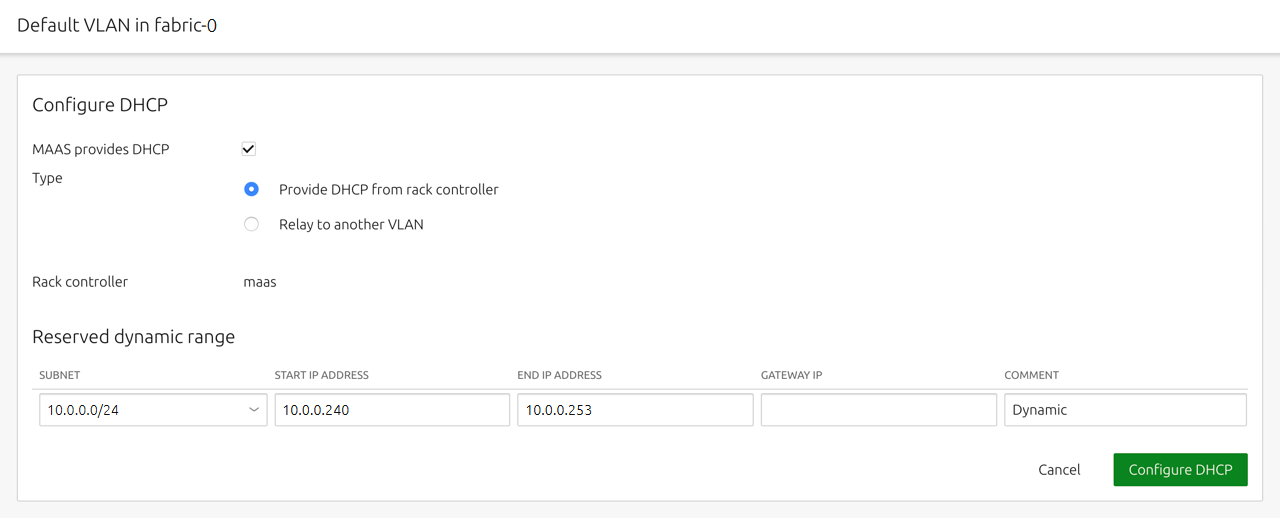
\includegraphics[width=1\linewidth]{tesi/files/immagini/maas/DHCP 240-253}
    \caption{Finestra di configurazione del DHPC.}
    \label{fig:maas_config_dhcp}
\end{figure}

\paragraph{Verifiche finali.}%\ \\%\noindent 
Ora il sistema MAAS è perfettamente funzionante.
% 
Per verificarlo basterà accedere alla schermata del controller appena configurato.
\begin{enumerate}
    \item[] 
    \begin{enumerate}
        \item Premere su "\emph{Controllers}" nel menù in alto, poi premere sul nome del controller desiderato (in questo caso \emph{maas.oscluster.unibo.it}).
        % 
        Verrà mostrata la schermata con le informazioni riguardanti il controller e lo status dei servizi in esecuzione.
        
        \item Verificare dunque che a fianco ai nomi di questi, come mostrato in \cref{fig:maas_sum_region+rack}, siano presenti le spunte verdi.
    \end{enumerate}
\end{enumerate}
% 
\begin{figure}[H]
    \centering
    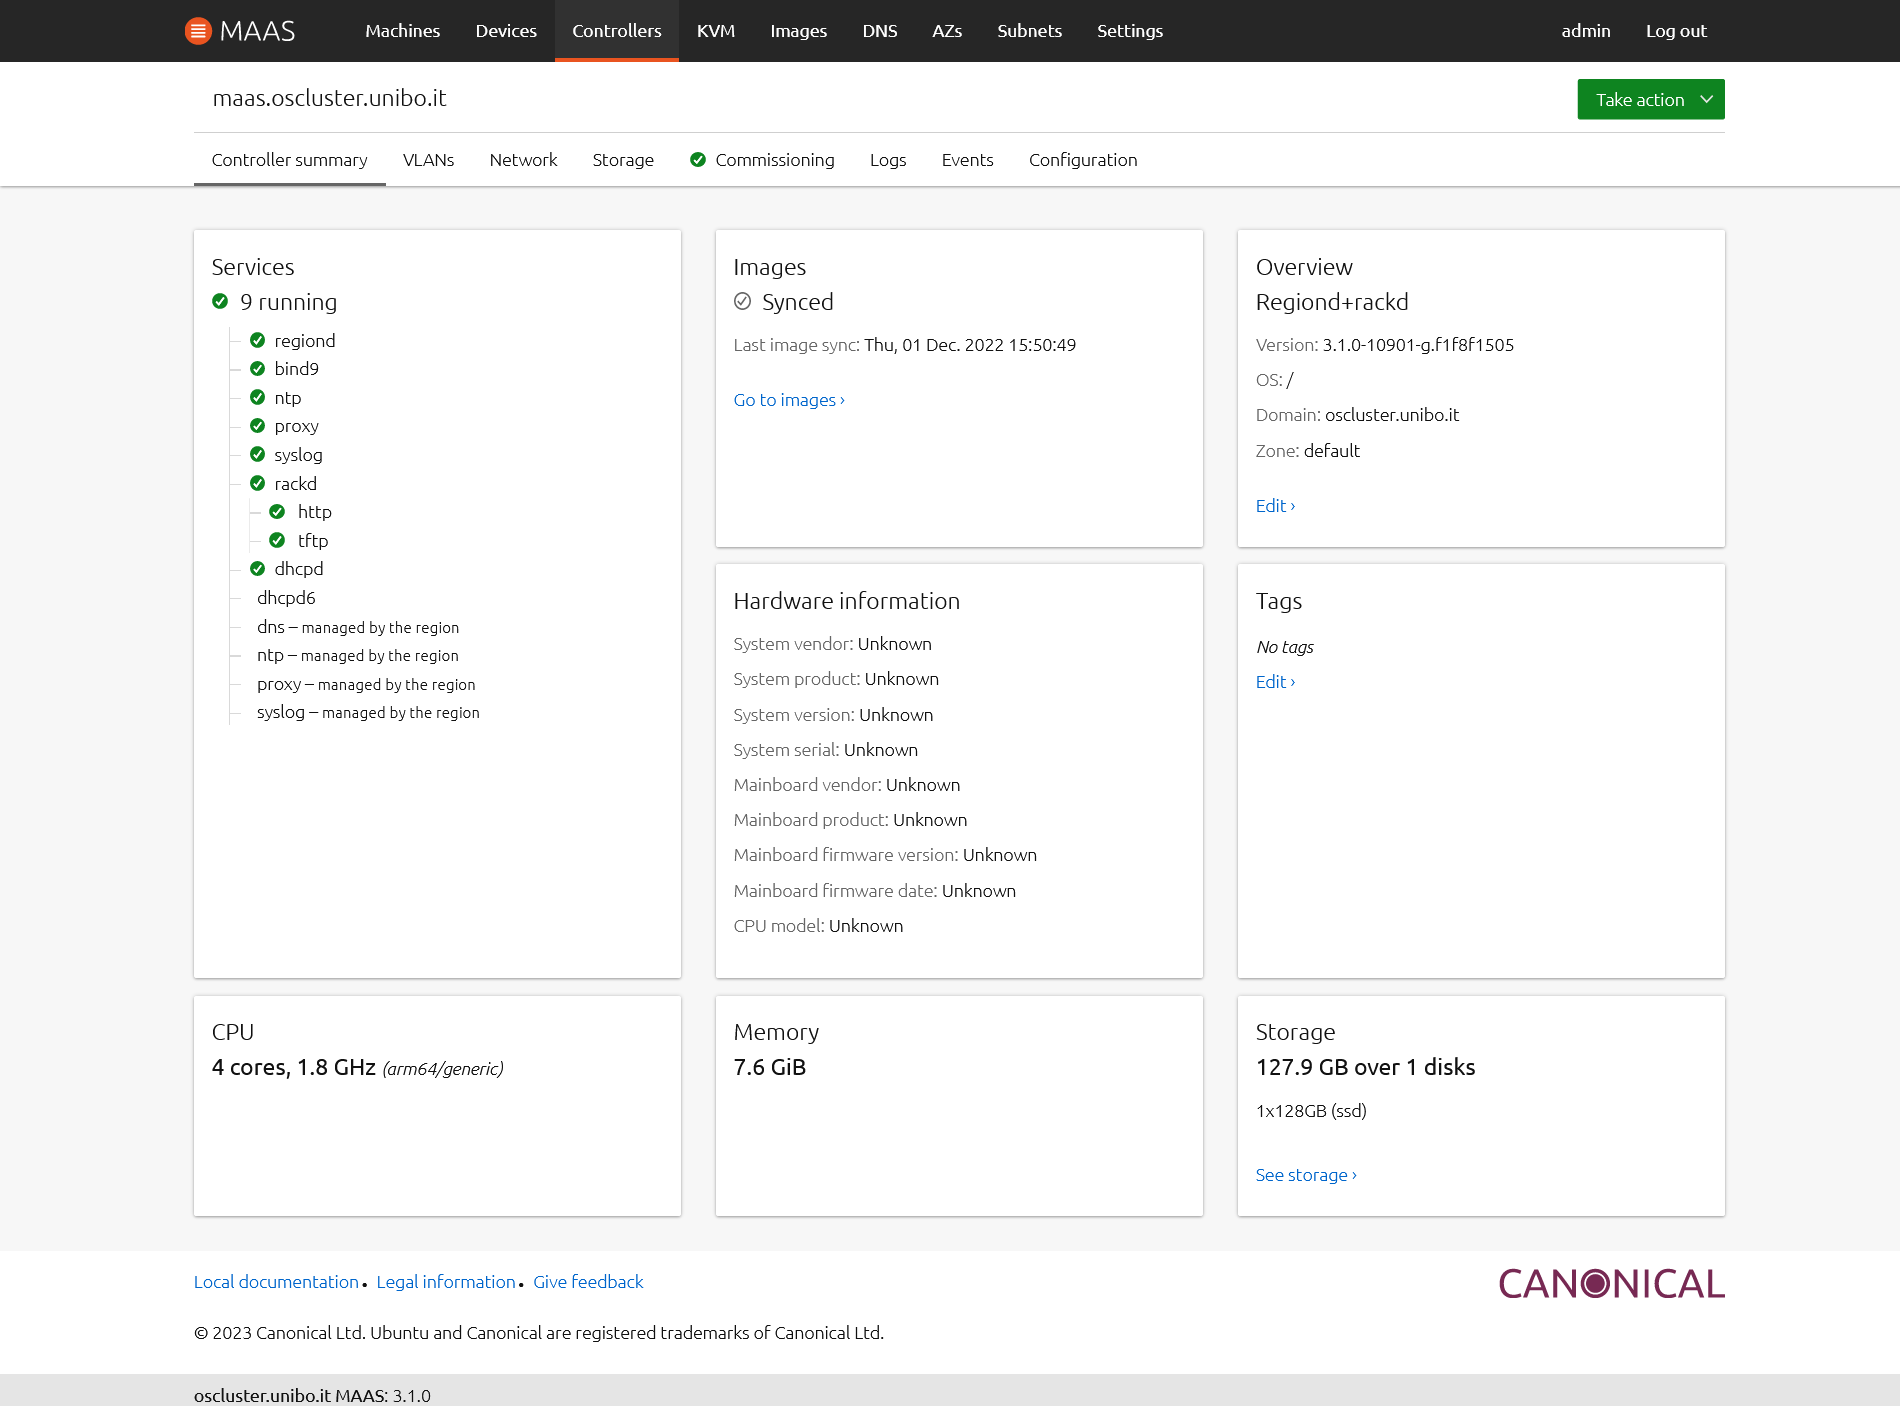
\includegraphics[width=1\linewidth]{tesi/files/immagini/maas/services_controller}
    \caption{Schermata di sintesi del region+rack controller.}
    \label{fig:maas_sum_region+rack}
\end{figure}
% 
% \paragraph{}
\bigskip
Come ultimo passaggio è consigliato verificare che le immagini selezionate nel punto \ref{itm:image_ubuntu} 
% di questa sezione
siano state scaricate correttamente.
\begin{enumerate}
    \item[] 
    \begin{enumerate}
        \item Premere su "\emph{Images}" nel menù in alto e nella schermata che comparirà.
        
        \item Verificare che le immagini scelte abbiamo come status "\emph{Synced}".
    \end{enumerate}
\end{enumerate}

\noindent
% CONFIGURAZIONE PROXY
Durante lo svolgimento del progetto sono sorti dei problemi con il Proxy HTTP integrato all'interno di MAAS.
% 
In particolare esso non permetteva alle macchine di collegarsi a internet e quindi di scaricare i software da installare e gli aggiornamenti.
% 
Dato che questa funzionalità non è strettamente necessaria per il funzionamento di tutto il sistema, è stato deciso di disabilitarla tramite la seguente procedura:
\begin{enumerate}
    \item Premere su "\textit{Settings}" nel menu in alto; in questo modo comparirà la schermata da cui è possibile modificare la configurazione del controller.
    
    \item Premere sul bottone "\textit{Proxy}" nella sottosezione "\textit{Network}".
    
    \item Selezionare la voce "\textit{Don't use a proxy}" e premere il tasto "\textit{Save}" per salvare le modifiche.
\end{enumerate}


\subsection{Aggiunta dei nodi}\label{subsubsec:maas_add_node}
Finalmente è possibile aggiungere le macchine al sistema.
% 
% Si ricordano i requisiti minimi dichiarati in AGGIUNGERE RIFERIMENTO per le singole macchine da collegare al sistema.
% 
% Inoltre 
Prima di procedere è importante verificare che nel BIOS di ciascuna macchina sia abilitata l'opzione \emph{PXE} (Preboot eXecution Environment), ovvero quella che permette il boot via rete e che sia 
in cima come priorità d'avvio.
% la prima come priorità.
% 
In caso di incertezze, consultare il manuale della scheda madre della macchina.

\bigskip
Nonostante la procedura per aggiungere i nodi possa essere eseguita simultaneamente, è consigliabile iniziare aggiungendo una macchina per volta in modo da prendere confidenza con i vari step e identificare correttamente le varie macchine.

Durante le seguenti fasi MAAS assocerà ai nodi uno status in base allo step del lifecycle; per maggiori dettagli si veda la \cref{subsubsec:maas_node}. 
% 
\begin{enumerate}
    \item \textbf{Enlist dei nodi.} Collegare la macchina alla subnet del rack controller e accenderla.
    % Accendere la macchina una volta che è stata collegata alla subnet del rack controller.
    % 
    Una volta effettuato il boot da rete, MAAS la rileva e avvia la procedura di enlist.
    % 
    A processo terminato la macchina si spegnerà e sarà possibile visualizzare il nodo appena aggiunto dall'interfaccia utente web di MAAS premendo su "\emph{Machines}" nel menù in alto. Il nodo appena aggiunto apparirà con status \emph{News}.

    \item\label{itm:powertype} \textbf{Configurazione power type.} La prima cosa da fare dopo aver aggiunto una macchina a MAAS è configurare il power type. Questo parametro indica la metodologia con la quale viene gestita l'alimentazione delle macchine. MAAS infatti ha la capacità di accendere e spegnere le macchine in autonomia nel caso queste siano predisposte (e.g. se sono dotate di una IPMI).

    È possibile configurare il power type di una macchina nel seguente modo:
    \begin{enumerate}
        \item Entrare nella schermata di visualizzazione delle macchine tramite il bottone "\emph{Machines}" nella barra di navigazione e cliccare sul nodo che si vuole configurare
        \item Aprire la scheda "\emph{Configuration}" e premere sul secondo tasto "\emph{Edit}" (quello riguardante la sezione \emph{Power configuration}).

        \item Selezionare il power type desiderato, configurarlo e al termine premere su "\emph{Save changes}" per applicare le modifiche.
    \end{enumerate}
    % 
    In questo scenario, dato che le macchine in dotazione non supportano l'avvio e lo spegnimento automatico, è stata scelta la modalità \emph{Manual}, che comporta una gestione manuale da parte dell'accensione e spegnimento delle macchine durante le varie fasi di setup.

    Per maggiori dettagli sulle varie tipologie messe a disposizione da MAAS, consultare la documentazione a riguardo \cite{maas_power_management}.

    \item \textbf{Rinominare i nodi.} È possibile rinominare i nodi, in modo tale che siano facilmente riconoscibili. Per fare questo è sufficiente entrare nella pagina di gestione del nodo, premere in alto a sinistra sul nome corrente e inserire quello nuovo; per salvare i cambiamenti è sufficiente premere invio o cliccare sul tasto "\emph{Save}".
    % 
    In questo scenario sono stati utilizzati nomi incrementativi per quanto riguarda i nodi, da \emph{node1} fino a \emph{node5}, mentre la macchina su cui verrà installato il controller Juju avrà semplicemente il nome \emph{juju}.

\end{enumerate}
% \paragraph
% \item[] \textbf{Commission.}
Una volta caricati tutti i nodi nel sistema, è possibile proseguire contemporaneamente su tutte le macchine.
\begin{enumerate}\setcounter{enumi}{3}
    \item \textbf{Commission.} MAAS ora è pronto per raccogliere le informazioni dei vari nodi.
    %
    Il tempo necessario al completamento di questa fase dipende da diversi fattori e potrebbe richiedere diversi minuti.
    \begin{enumerate}
        \item Dalla  pagina "\emph{Machines}" selezionare tutti i nodi spuntando la casella a sinistra del loro nome.
        
        \item Premere sul pulsante verde "\emph{Take action}" in alto a destra e poi premere su "\emph{Commission...}". %causa sbordo di 2 caratteri e non va a capo da solo, causando warning; vedere se aggiungere forzamento a capo prima dell'emph con \\
        
        \item A questo punto, se nel punto \ref{itm:powertype} il power type dei nodi è stato configurato su \emph{Manual}, bisognerà accendere tutti i nodi manualmente.
        % 
        Una volta completata la fase di commission, i computer si spegneranno e i nodi passeranno in stato \emph{Commissioned}.
    \end{enumerate}
    
    \item\label{itm:tag_node} \textbf{Tag dei nodi.} È possibile associare ai nodi delle etichette per facilitarne la selezione e gestione durante le fasi di installazione del cloud.
    % 
    \begin{enumerate}
        \item[] Dalla  scheda "\emph{Configuration}" di un singolo nodo, premere sul primo tasto "\emph{Edit}" e nella casella di testo "\emph{Tags}" aggiungere i tag desiderati. 
    \end{enumerate}
    % 
    In questo scenario sono stati utilizzati il tag \emph{compute} per i nodi del cloud (eccetto per il node5 al quale non è stato associato alcun tag) e il tag \emph{juju} per la macchina con il controller Juju. 

    \item\label{itm:maas_ovs_bridge} \textbf{Creazione del OvS bridge.} Come ultimo passaggio, è importate creare uno switch virtuale su ogni nodo del cloud (non la macchina juju) che verrà successivamente utilizzato per poter collegare le VM alla rete esterna.
    % 
    Per maggiori dettagli su Open vSwitch, vedasi la \cref{subsubsec:ovs}.
    \begin{enumerate}
        \item Dalla  pagina del nodo aprire la scheda "\emph{Network}", spuntare la casella a fianco al nome della rete e premere sul tasto "\emph{Create bridge}".

        \item A questo punto compare la finestra per la configurazione del OvS bridge; inserire un nome in "\emph{Bridge name}" uguale per tutti i nodi, selezionare in "\emph{Bridge type}" il valore \emph{Open vSwitch (ovs)}, inserire i parametri di rete corretti (come il  "\emph{Fabric}",  "\emph{VLAN}", "\emph{Subnet}") e in "\emph{IP mode}" selezionare \emph{Auto assign} per l'assegnamento automatico degli indirizzi IP.
    \end{enumerate}

    In \cref{fig:maas_ovs} viene mostrata la configurazione usata in questo scenario su uno dei quattro nodi del cloud;
    % 
    eccetto per il campo "\emph{MAC address}", la configurazione risulta essere la medesima per ogni nodo.
    % \end{itemize}
\end{enumerate}

\begin{figure}[H]
    \centering
    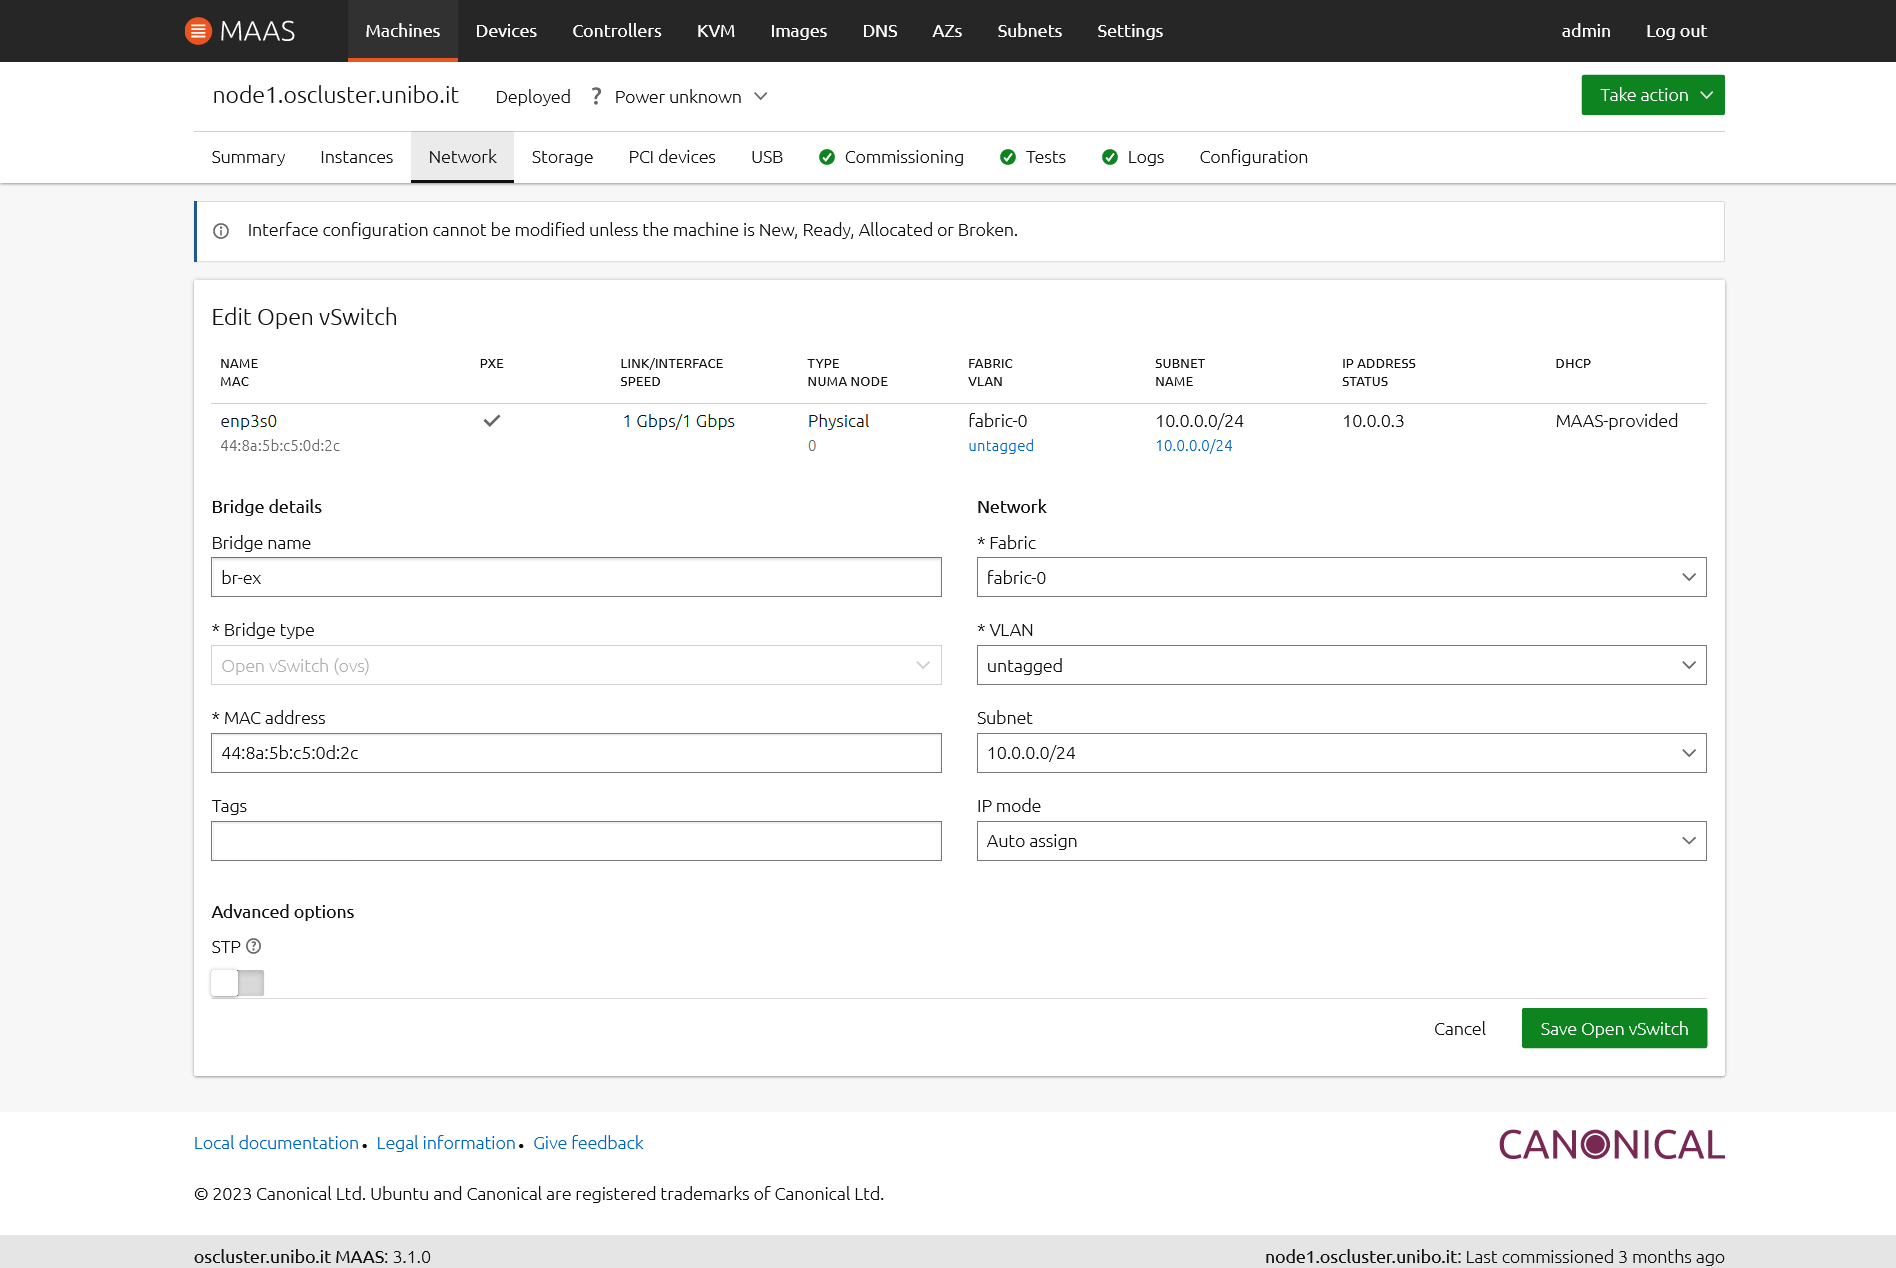
\includegraphics[width=1\linewidth]{tesi/files/immagini/maas/ovs}
    \caption{schermata di editing della configurazione Open vSwitch su un nodo.}
    \label{fig:maas_ovs}
\end{figure}


\bigskip\bigskip\noindent
L'installazione e la configurazione di MAAS è terminata.
% 
Il prossimo passo sarà quello di introdurre e installare il sistema Juju, il quale consentirà il deploy e la gestione lato software sui vari nodi. 

% 

\newpage

\section{Juju}\label{subsec:juju}
Juju \cite{juju_home} è un sistema open source adibito all'automazione, configurazione e deploy di infrastrutture e software per cloud ibridi e non.
% 
Sviluppato anch'esso da Canonical, ha come compito quello di aiutare gli amministratori di sistema nel deploy e semplificare la gestione software del cloud, spostando l'attenzione dalla gestione delle configurazioni delle applicazioni alla gestione delle applicazioni stesse.
% 
In questo modo i progettisti di sistemi cloud possono concentrarsi maggiormente sull'amministrazione ad alto livello delle applicazioni e degli scenari, sviluppando modelli per gestire il ridimensionamento, il coordinamento  e le dipendenze tra i vari servizi.

Aumento della scalabilità e della ridondanza, semplificazione nella gestione dell'infrastruttura e architettura del cloud e automazione nel deploy sono esempi dei vantaggi che si hanno utilizzando Juju nella creazione dei cloud.

Inoltre è possibile utilizzare Juju per gestire ambienti multi-cloud, ovvero l'utilizzo di più provider di cloud contemporaneamente, come ad esempio AWS (Amazon Web Services) per la parte computazionale e GCP (Google Cloud Platform) per lo storage.

Infine Juju può anche operare in ambienti diversi dai consueti cloud gestendoli comunque come se fossero dei veri e propri cloud, 
% ma continuando a gestire il software come se si trattasse di un cloud,
ad esempio server bare metal utilizzando MAAS o container utilizzando LXD.
% 
Questa tipologia di cloud viene anche definita \emph{substrate} \cite{juju_cloud_substrate}.



\subsection{Funzionamento: Controller e Charmed Operator}\label{subsec:juju_funzionamento}
\paragraph{Controller.} Il controller \cite{juju_controller} è il core di Juju nella gestione del cloud.
% 
Ha come compito quello di creare e gestire l'infrastruttura software del cloud ed è il responsabile dell'implementazione di tutte le modifiche richieste da parte del client Juju.
% 
Ogni controller generalmente è situato su una macchina dedicata e gestisce un singolo cloud (\cref{fig:juju_client_controllers}), quest'ultimi sono descritti attraverso i modelli.
% 
\begin{figure}[H]
    \centering
    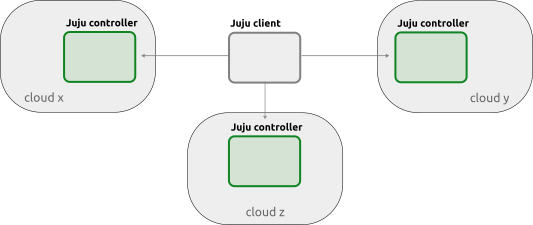
\includegraphics[width=0.8\linewidth]{tesi/files/immagini/juju/client_controllers}
    \caption{Schema del sistema Juju. Un Juju client può comunicare con più Juju controller \cite{juju_client}.}
    \label{fig:juju_client_controllers}
\end{figure}

\noindent
Un \textbf{modello} \cite{juju_model} è una collezione di applicazioni distribuite all'interno di diverse macchine.
% 
Il suo scopo è quello di consentire il raggruppamento logico di applicazioni e infrastrutture che operano e collaborano assieme per fornire un determinato servizio. 
% 
Un modello è gestito da un singolo controller, mentre un controller può gestire diversi modelli e quindi diversi set di applicazioni e macchine.

Alla creazione del controller vengono generati due modelli: il modello \emph{controller}, che conterrà solamente la macchina del controller, e il modello \emph{default}, un modello generico utilizzabile per distribuire applicazioni e macchine.
% 
\begin{figure}[H]
    \centering
    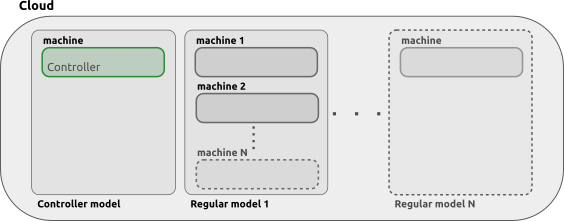
\includegraphics[width=0.8\linewidth]{tesi/files/immagini/juju/models}
    \caption{Rappresentazione del cloud in modelli. Un singolo Controller model e diversi Regular model su diverse macchine \cite{juju_model}.}
    \label{fig:juju_models}
\end{figure}
% 
\noindent 
In sintesi, un cloud è composto da un controller che gestisce vari modelli e ogni modello distribuisce applicazioni su diverse macchine (\cref{fig:juju_models}).
 

\paragraph{Charmed Operator.}
Un Charmed Operator \cite{juju_charm}, o più semplicemente \emph{Charm}, è un componente software open source che guida le fasi del ciclo di vita di una singola applicazione in tutti i suoi aspetti, come l'installazione, distribuzione, configurazione, aggiornamenti e interoperabilità con altre applicazioni.
% 
Ne gestisce inoltre le istanze, il ridimensionamento, l'ottimizzazione, il networking, semplificando la distribuzione dell'applicazione, rendendola facilmente riutilizzabile e condivisibile.

I charm sono un'espansione e una generalizzazione della nozione di operatore in Kubernetes, con la differenza che le applicazioni possono essere connesse ad altre applicazioni e possono essere distribuite non solo su cluster Kubernetes ma anche su container, VM, e macchine bare metal, sia su cloud pubblico che privato.

Esiste un'altra tipologia di charm, chiamato \emph{subordinate charmed operator}, che aumenta le funzionalità di un altro charm già esistente (in questo contesto viene denominato come \emph{principal charmed operator}).
Quando un subordinate charm viene distribuito, non viene creata una nuova istanza dell'applicazione a cui fa riferimento il principal charmed ma ne estende direttamente le funzionalità.

\bigskip
I charm sono orchestrati dal componente integrato in Juju chiamato \emph{Charmed Operator Lifecycle Manager (OLM)} \cite{juju_olm} .
% 
Questo strumento ha il compito di distribuire e mantenere aggiornate le applicazioni che i charm descrivono, provvedendo al deploy delle varie istanze delle applicazioni nelle macchine del cloud.
% 
Quando vengono scelti in fase di deploy, i charm vengono scaricati dal marketplace \emph{Charmhub} \cite{charmhub}, il luogo dove è possibile sviluppare e condividere gratuitamente i propri charm.

\subsection{Concetti chiave}\label{subsec:juju_concetti}
\paragraph{Bundle.}
% https://juju.is/docs/sdk/charm-bundles
Un bundle \cite{juju_bundle} è la rappresentazione di un modello Juju in un file in formato yaml.
% 
Al suo interno sono elencati tutti i charm, le relazioni e le configurazioni per poter effettuare il deploy del modello che rappresenta.
% 
Infatti partendo da un bundle, è possibile effettuare il deploy in maniera automatizzata di un modello, rendendolo un potente strumento indispensabile per la distribuzione di sistemi grandi e complessi in modo semplice e ripetibile.
% 
Come per i charm, è possibile trovare bundle già costruiti da altri utenti in maniera veloce e gratuita nel marketplace \emph{Charmhub} \cite{charmhub}.

\paragraph{Overlay.}
Un overlay è un'estensione del bundle.
% 
Anch'esso in formato yaml, il suo compito è quello di permettere la personalizzazione di un bundle esistente senza dover applicare direttamente le modifiche sul file, lasciando quindi inalterato l'intero bundle.
% 
In questo modo è possibile utilizzare un bundle più generico ed applicare delle personalizzazioni tramite overlay, per esempio aggiungendo charm o impostando dei vincoli personalizzati sulle macchine, o ancora modificando il numero di macchine su cui distribuire determinate applicazioni.

\paragraph{Unit.}
% https://juju.is/docs/olm/unit
Juju definisce le unit \cite{juju_unit} come le istanze di un'applicazione in esecuzione e ognuna di queste viene istanziata su macchine distinte.
% 
Durante il deploy è possibile decidere quante e su quali macchine installare le unit.
% 
Grazie alle unit è possibile dividere una singola applicazione in più istanze, garantendo in questo modo un set di repliche resiliente ai guasti e una suddivisione del carico di lavoro.
% 
Ad esempio, come mostrato in \cref{fig:juju_units} è possibile distribuire il charm mongodb su tre macchine, specificando in fase di deploy sia il numero di unit sia le macchine di destinazione.
% 
Ogni unit viene contraddistinta da un numero, preceduto dal nome dell'applicazione;
% 
ad esempio la prima unit verrà denominata "nome\_app/0".
% 
Infine, tutte le unit della stessa applicazione condividono lo stesso codice del charm, le stesse relazioni e le stesse configurazioni, ma una di esse verrà battezzata come "leader" e sarà responsabile della gestione del lifecycle dell'intera applicazione.
\begin{figure}[H]
    \centering
    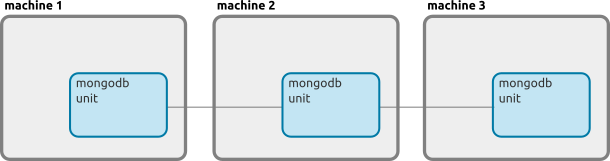
\includegraphics[width=0.8\linewidth]{tesi/files/immagini/juju/units}
    \caption{Suddivisione dell'applicazione MongoDB su tre unit \cite{juju_unit}.}
    \label{fig:juju_units}
\end{figure}


\paragraph{Relation.}
% Da Juju 3.0 si chiamano Integration
% https://juju.is/docs/olm/integration
Una relation \cite{juju_relation} (integration dalla versione 3.0 di Juju) è un protocollo di Juju che facilita lo scambio di informazioni e configurazioni tra applicazioni.
% 
Le relation di un'applicazione sono definite all'interno del charm e vengono create connettendo i vari endpoint delle applicazioni coinvolte.
% 
I vari endpoint possono essere connessi solamente se sono dello stesso tipo e se supportano la stessa interfaccia.
% 
Per esempio, come mostrato in \cref{fig:juju_relations}, il charm wordpress necessita di un database e fornisce un sito web, quindi espone rispettivamente le interfacce "mysql" e "http", alle quali è possibile (e necessario) collegare i charm mysql e apache attraverso le loro rispettive interfacce che a loro volta mettono a disposizione.

\begin{figure}[H]
    \centering
    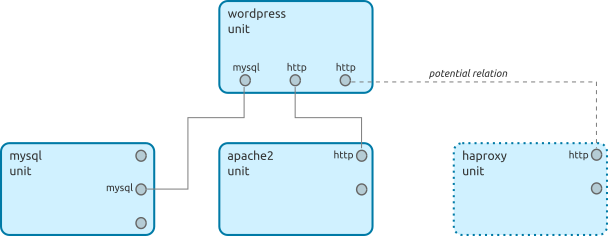
\includegraphics[width=0.9\linewidth]{tesi/files/immagini/juju/relations}
    \caption{WordPress in relation con MySQL e Apache (eventualmente anche con HAProxy) \cite{juju_relation}.}
    \label{fig:juju_relations}
\end{figure}

\noindent
Le relation possono essere facoltative o obbligatorie, a seconda delle dipendenze che charm necessita e di come è stato definito dal suo creatore.
% 

Va evidenziato che le relation non sono connessioni dirette tra i vari charm, bensì una virtualizzazione delle connessioni per consentire lo scambio di informazioni di configurazioni.
% 
Infatti è il controller Juju che ha il ruolo di mediatore per queste connessioni virtuali, gestendo il vario flusso di informazioni tra dli accessi. 

% \paragraph{Agent.}



\subsection{Installazione}\label{subsubsec:juju_install}
\paragraph{Preparazione Hardware.}
Come anticipato nella \cref{subsec:progettazione_hardware}, il  sistema cloud  progettato in questa tesi è costituito da:
\begin{itemize}
    \item Una macchina dedicata (Raspberry Pi) per il sistema MAAS (vedasi deploy nella \cref{subsubsec:maas_install}), a cui in questo capitolo verrà aggiunto il client Juju.

    \item Una macchina dedicata per il controller Juju.
    
    \item Quattro nodi sui quali verrà effettivamente installato il cloud OpenStack più un quinto per sviluppi successivi.
\end{itemize}
% 
In questo capitolo verrà trattata la sola installazione del sistema Juju, composto dal client e dal controller.

\paragraph{Preparazione software.}
L'installazione di Juju affrontata in questa sede è affiancata dallo strumento di provisioning server MAAS (\cref{subsec:maas}).
% 
Inoltre, è altre sì importante che la macchina dedicata al controller Juju sia stata aggiunta all'elenco dei nodi gestiti da MAAS (fase di elinst e commission)
% 
Pertanto, prima di procedere, è necessaria effettuare l'installazione completa del suddetto strumento e l'aggiunta dei nodi.
% 
Si vedano le \cref{subsubsec:maas_install,subsubsec:maas_conf,subsubsec:maas_add_node} per maggiori dettagli.

\bigskip
La versione di Juju che è stata installata è la 2.9.29, aggiornata poi alla 2.9.37.
% 
Il comando che verrà utilizzato in fase di installazione però installerà l'ultima versione disponibile;
% 
ciò non dovrebbe risultare problematico, ma è bene prestare attenzione che alcuni aspetti potrebbero essere differenti se si vorrà installare una versione più aggiornata.
% 
È comunque possibile, come verrà descritto poi nel \cref{lst:juju_client_install}, decidere quale versione scaricare e installare.


\paragraph{N.B.} Rispetto ad un'installazione da manuale basata sul sistema operativo Ubuntu 20.04 con architettura AMD64, quella affrontata in questa sede differisce leggermente essendo basata sul sistema operativo Raspberry Pi OS (Debian 11) con architettura ARM64.
% 
Tutte le eventuali differenze riscontrate verranno spiegate e mostrate nei dettagli.

\bigskip\noindent
 Per maggior informazioni sulle seguenti fasi di installazione, fare riferimento alla guida OpenStack \cite{juju_install_openstack} e alla documentazione Juju \cite{juju_install_doc,juju_use_maas}. %e \cite{juju_use_maas}
 % https://juju.is/docs/olm/install-juju
 % https://juju.is/docs/olm/configure-a-model
 
\subsection{Installazione e configurazione del client Juju}
Durante le fasi di installazione di Juju verranno utilizzati solamente comandi da terminale impartiti sulla macchina Raspberry Pi del sistema MAAS, diventando così anche client Juju.

\bigskip\noindent
Come prima cosa verrà installato il client Juju all'ultima versione. %alla versione 2.9.37
\begin{lstlisting}[
    language=mybash, 
    caption={Installazione del client Juju.}, 
    label={lst:juju_client_install}
]
sudo snap install ^nf^juju^nf^ --classic
\end{lstlisting}

Nel caso in cui si volesse installare un'altra versione, è possibile specificarla aggiungendo \code{-{}-channel=<version/release>}.
    Per esempio, per la versione \code{2.9.37} si va ad aggiungere \code{-{}-channel=2.9.37/stable}.

\bigskip\noindent
Fatto ciò, MAAS verrà collegato a Juju in modo tale che venga visto e gestito come se fosse un cloud.
% 
Prima verrà creato un file yaml di nome \emph{mass-cloud.yaml} contenente le seguenti configurazioni del cloud MAAS.
% 
\lstinputlisting[
    language=yaml, 
    caption={File yaml di configurazione del cloud MAAS.}, 
    label={lst:juju_maas-cloud-yaml},
]
{tesi/files/installazioni/yaml/juju/maas-cloud.yaml}
%
\begin{itemize}
    \item La dicitura \code{mass-one} indica il nome che assumerà il cloud.
    % 
    Se si vuole utilizzare un altro nome, bisogna cambiare la dicitura \code{mass-one} con il nome desiderato.

    \item In \code{type} viene indicato la tipologia del cloud; in questo caso \texttt{maas}.

    \item Con \code{auth-types} si intende il tipo di autenticazione del cloud (verrà aggiunta la chiave di autenticazione nei \cref{lst:juju_maas-creds-yaml,lst:juju_add-credential}).

    \item \code{endpoint} invece è l'URL, il punto d'accesso di MAAS inserito in fase di installazione nel \cref{lst:maas_init}.
\end{itemize}

\bigskip\noindent
A questo punto è possibile aggiungere il cloud a Juju.
% 
\begin{lstlisting}[
    language=mybash, 
    caption={Aggiunta del cloud mass-one in Juju.}, 
    label={lst:juju_add-cloud},
]
juju add-cloud --client -f maas-cloud.yaml maas-one
\end{lstlisting}
%
\begin{itemize}
    \item Con l'opzione \code{-{}-client} si va ad indicare a Juju di archiviare la definizione del cloud sulla macchina da cui si sta eseguendo il comando, ovvero il client Juju
    
    \item Con l'argomento \code{-f} viene indicato il nome del file di configurazione yaml salvato nel \cref{lst:juju_maas-cloud-yaml}
    \item Il valore \emph{mass-one} indica il nome del cloud corrispondente a quello scelto sempre nel \cref{lst:juju_maas-cloud-yaml}.
\end{itemize}
% 
Per verificare che il cloud sia stato correttamente aggiunto, si può eseguire \code{juju clouds -{}-client}; 
% 
l'output dovrebbe essere simile a quello mostrato in \cref{fig:juju_cloud_mass-one}.
% 
\begin{figure}[H]
    \centering
    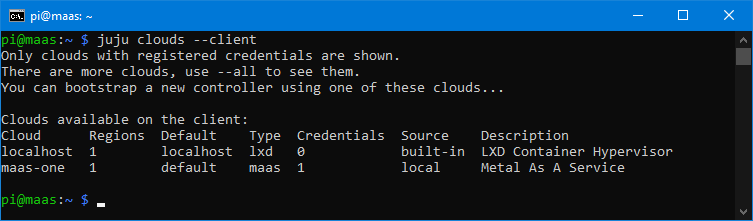
\includegraphics[width=1\linewidth]{tesi/files/immagini/juju/juju clouds}
    \caption{Elenco dei cloud presenti nel sistema Juju.}
    \label{fig:juju_cloud_mass-one}
\end{figure}

\bigskip\noindent
Una volta aggiunto il cloud MAAS, Juju ha bisogno delle credenziali per poter interagire con esso.
Verrà creato un nuovo file yaml ad hoc di nome \emph{maas-creds.yaml} avente le seguenti impostazioni.
% 
\lstinputlisting[
    language=yaml, 
    caption={File yaml contenente le credenziali del cloud MAAS.}, 
    label={lst:juju_maas-creds-yaml},
]
{tesi/files/installazioni/yaml/juju/maas-creds.yaml}
%
\begin{itemize}
    \item \code{mass-one} è il nome del cloud scelto nel \cref{lst:juju_maas-cloud-yaml}.

    \item \code{anyuser} è il nome del nuovo utente che Juju andrà ad utilizzare.

    \item Con \code{auth-type} si indica la tipologia delle credenziali da inserire.

    \item Infine in \code{maas-oauth} va indicata la chiave API che è stata salvata nel \cref{lst:maas_apikey};
    % 
    quindi sostituire \emph{admin-api-key-file} con la corrispondente chiave.
\end{itemize}

\bigskip\noindent
Ora è possibile aggiungere le credenziali a Juju.
% 
\begin{lstlisting}[
    language=mybash, 
     caption={Aggiunta delle credenziali del cloud MAAS in Juju.}, 
    label={lst:juju_add-credential},
]
juju add-credential --client -f maas-creds.yaml maas-one
\end{lstlisting}
% 
\begin{itemize}
    \item[] (Vedasi il \cref{lst:juju_add-cloud} per la spiegazione degli argomenti del comando eseguito).
\end{itemize}
% 
Anche in questo caso è possibile verificare che le credenziali siano state inserite correttamente.
% 
Per farlo, basterà eseguire \code{juju credentials -{}-client}\\\code{ -{}-show-secrets -{}-format yaml}; l'output dovrebbe essere simile a quello illustrato in \cref{fig:juju_credentials}.
% 
\begin{figure}[H]
    \centering
    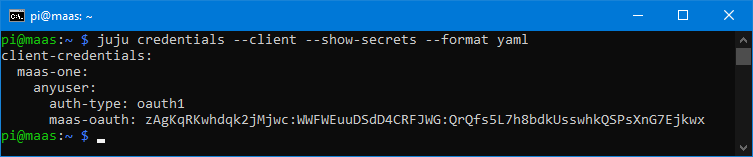
\includegraphics[width=1\linewidth]{tesi/files/immagini/juju/juju credentials}
    \caption{Elenco delle credenziali presenti nel sistema Juju.}
    \label{fig:juju_credentials}
\end{figure}

\bigskip
\subsection{Deploy del controller Juju e creazione del model}\label{sec:juju_model_create}
Arrivati a questo punto, è possibile avviare il deploy automatizzato del controller Juju.
% 
Tale richiesta verrà demandata a MAAS, il quale si occuperà dell'installazione del sistema operativo e del controller.
\begin{lstlisting}[
    language=mybash, 
    caption={Deploy del controller Juju nella macchina con tag juju.}, 
    label={lst:juju_bootstrap},
]
juju bootstrap ^c^--bootstrap-series=^c^focal --constraints "^c^tags=^c^^nf^juju^nf^ ^c^arch=^c^amd64" maas-one maas-controller
\end{lstlisting}
% \lstinputlisting[
%     language=mybash, 
%     caption={Deploy del controller Juju nella macchina con tag juju.}, 
%     label={lst:juju_bootstrap},
%     firstline=4,
%     lastline=4
% ]
% {tesi/files/installazioni/CLI/juju}
%
\begin{itemize}
    \item Con l'opzione \code{-{}-bootstrap-series} viene specificata la versione dell'immagine del sistema operativo da far installare da MAAS;
    questa verrà presa tra le immagini scaricate nel \cref{itm:image_ubuntu} nella \cref{subsubsec:maas_conf}.

    In questo caso è stata installata Ubuntu Focal, corrispondente alla versione 20.04 LTS.

    \item Con l'opzione \code{-{}-constraints} è possibile specificare in maniera precisa l'hardware a cui si sta facendo riferimento.
    % 
    In caso di più valori, questi devono essere inseriti all'interno del carattere doppio apice come mostrato nel \cref{lst:juju_bootstrap}.
    
    In questo caso è stato indicato col valore \code{tag=juju} che il comando deve essere eseguito per il nodo con il tag "juju".
    
    Inoltre, in questo specifico scenario, si è rilevato indispensabile aggiungere anche il valore \code{arch=amd64}, in quanto il comando \code{bootstrap} viene richiesto dal client Juju, situato su Raspberry Pi avente architettura ARM64 e non AMD64 come per i restanti nodi.

    Dunque in uno scenario diverso da quello presentato in questo documento, se tutte le architetture di tutte le macchine coinvolte saranno di tipo AMD64 non sarà necessario l'aggiunta del suddetto valore.

    \item \emph{mass-one} è il nome del cloud scelto nel \cref{lst:juju_maas-cloud-yaml}, mentre \emph{maas-controller} sarà il nome che assumerà il controller Juju, ovvero il controller del cloud.

\end{itemize}
% 
A comando avviato, dall'interfaccia utente web di MAAS (\cref{subsubsec:maas_conf}) dalla schermata "\emph{Machines}" sarà possibile verificare lo stato di avanzamento della fase di deploy.

Se durante la configurazione del power type dei nodi (\cref{itm:powertype} nella \cref{subsubsec:maas_add_node}) è stata scelta la modalità \emph{Manual}, la macchina del controller Juju deve essere avviata manualmente.
% 
L'intera fase di deploy richiede all'incirca una decina di minuti.
% 
A deploy terminato, la macchina del controller Juju si spegnerà e apparirà nell'elenco dei nodi sotto lo status \emph{Deployed}.

Per visualizzare l'elenco aggiornato dei controller noti al client Juju, eseguire il comando \code{juju controllers}, il cui output d'esempio viene mostrato in \cref{fig:juju_controllers}.
% 
\begin{figure}[H]
    \centering
    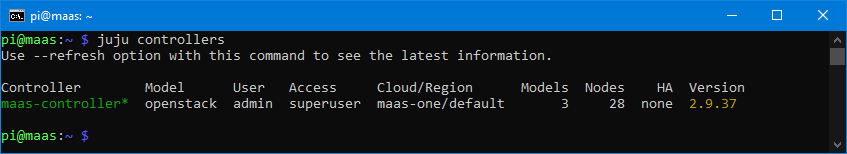
\includegraphics[width=1\linewidth]{tesi/files/immagini/juju/juju controllers}
    \caption{Elenco dei controller registrati nel client Juju.}
    \label{fig:juju_controllers}
\end{figure}

\bigskip\noindent
L'ultimo passo è quello di creare il model del cloud, al quale successivamente verranno aggiunti i vari charm che daranno corpo all'istanza effettiva del cloud.
\begin{lstlisting}[
    language=mybash, 
    caption={Creazione del model openstack per il cloud mass-one.}, 
    label={lst:juju_add-model},
]
juju add-model --config ^c^default-series=^c^jammy openstack
\end{lstlisting}
% 
\begin{itemize}
    \item Con l'opzione \code{-{}-config} è possibile specificare varie configurazioni al modello.
    Con il valore \code{default-series=} viene indicata l'immagine di default da utilizzare in fase di deploy dei nodi all'interno del cloud.
    In questo caso, l'immagine del sistema operativo è Ubuntu Jammy, corrispondente alla versione 22.04 LTS.
    
    \item Il valore \emph{openstack} sta ad indicare il nome che assumerà il model.
\end{itemize}
% 
Al termine, eseguendo il comando \code{juju status} è possibile verificare la creazione del cloud.
% 
Come mostrato in \cref{fig:juju_status1} l'output riassume il cloud appena creato.
% 
\begin{figure}[H]
    \centering
    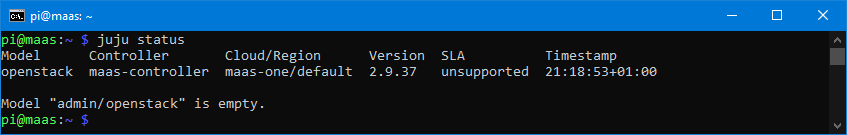
\includegraphics[width=1\linewidth]{tesi/files/immagini/juju/juju status1}
    \caption{Status del cloud vuoto mass-one.}
    \label{fig:juju_status1}
\end{figure}

\bigskip\noindent
%In \cref{sec:appendice_juju} è possibile visionare l'elenco dei comandi precedentemente descritti in un unico listato.


% accesso alla dashboard di juju
\subsection{Accesso alla dashboard}
Una volta effettuata l'installazione di Juju, è possibile accedere alla dashboard grafica attraverso il browser web.
% 
Infatti, come per MAAS, è disponibile una web app, che permette di monitorare le varie applicazioni e i vari charm all'interno del model del cloud.
% 
Eseguendo quindi il comando \code{juju dashboard} verrà mostrato L'URL per accedere all'interfaccia web, lo username e la password da utilizzare.
% 
In questo caso, l'URL dell'interfaccia web è:
% 
\begin{itemize}
    \item[]URL: \texttt{https://10.0.0.254:17070/dashboard}
\end{itemize}
% 
Mentre le credenziali da immettere sono:
% 
\begin{itemize}
    \item[]Username: \texttt{admin}

    \item[]Password: \texttt{527460c1b6b309a6bfd565924bcaacf4}
\end{itemize}

\bigskip\noindent
L'uso della dashboard è del tutto superfluo, e in questo documento non verrà ulteriormente menzionata.
% 
Tuttavia, può risultare comoda nel momento in cui si voglia andare a configurare qualche charm nello specifico;
% 
questo perché vengono mostrati direttamente le possibili configurazioni e azioni che questi possano avere, senza doverli cercare ne in documentazione ne a riga di comando.

In \cref{fig:juju_dashboard} viene mostrata la schermata d'accesso del cloud OpenStack con i charm già installati.
% 
Come è possibile vedere sono presenti sia i due model che vengono creati in automatico, ovvero il model per il \emph{controller} e il model di \emph{default}, che il model \emph{openstack}, creato nel \cref{lst:juju_add-model}.

\begin{figure}[H]
    \centering
    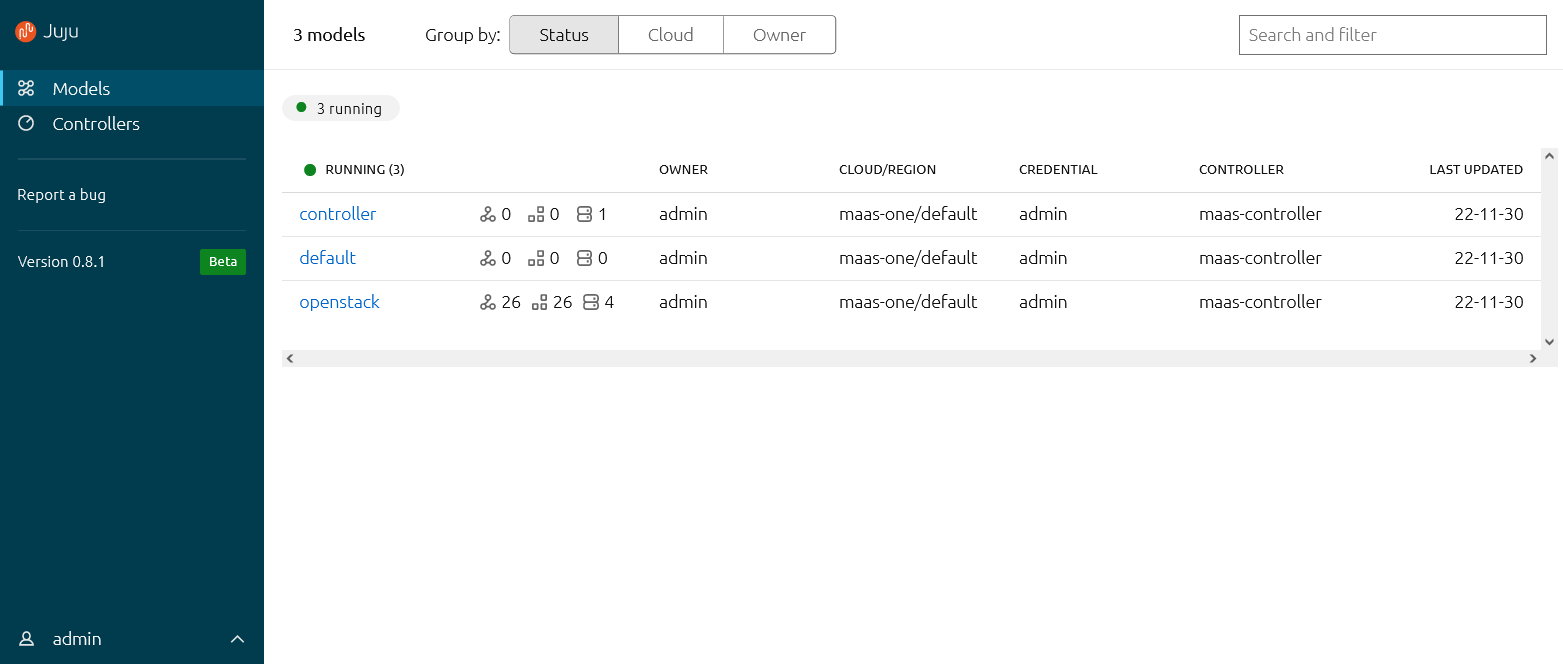
\includegraphics[width=1\linewidth]{tesi/files/immagini/juju/juju_dashboard.png}
    \caption{Esempio di schermata d'accesso della Juju dashboard.}
    \label{fig:juju_dashboard}
\end{figure}

\bigskip\noindent
Nei prossimi capitolo verrà trattata la piattaforma OpenStack, partendo da una sua descrizione e composizione, per poi passare alla completa installazione del cloud fino ad arrivare ad un suo semplice utilizzo.

\newpage

\chapter{OpenStack}

OpenStack è una piattaforma di cloud computing completamente open source. Viene largamente utilizzata sia da aziende che vogliono costruirsi un proprio cloud privato che da cloud provider che offrono i loro servizi a terzi.
Una caratteristica fondamentale di OpenStack è che non è un software monolitico, ma è composto da numerosissimi componenti che permettono un'ampia personalizzazione; è possibile infatti decidere quali componenti installare in base alle funzionalità che si desiderano e su quale macchina fisica installare ciascun componente in modo che si possano costruire macchine con caratteristiche diverse in base al componente che devono ospitare (e.g. la macchina che deve contenere il componente di block storage sarà sicuramente diversa rispetto ad una che deve contendere l'hypervisor).
Oltre ai propri componenti, OpenStack utilizza anche software di terze parti, che verrà approfondito nel capitolo \ref{sec:openstack_external_components}.

\section{Componenti di OpenStack}

Di seguito verranno descritti i componenti di OpenStack che sono stati installati durante questo progetto di tesi. Esistono numerosi altri componenti che implementano altre funzionalità ma, dato che non sono stati installati o approfonditi durante lo svolgimento del progetto, non verranno trattati.

\subsection{Cinder}\label{sec:openstack_cinder}
Cinder è il servizio di block storage di OpenStack e il suo compito è quello di fornire API di block storage sia agli utenti che agli altri componenti di OpenStack. Una sua caratteristica fondamentale è che virtualizza l'accesso ai dispositivi di storage in modo che i client possano utilizzare le API che espone senza sapere quale sia il backend utilizzato. Di conseguenza Cinder non implementa al suo interno la gestione fisica dello storage ma si collega a sua volta ad altri servizi come ad esempio OpenStack Swift o Ceph (quello utilizzato in questo progetto).

\subsection{Glance}\label{sec:openstack_glance}
Glance è il servizio di immagini di OpenStack, ovvero il servizio che si occupa di scoprire, registrare e fornire le immagini di macchine virtuali e i relativi metadati. Questo componente espone una serie di API che permettono di consultare i metadati di ciascuna immagine e di prelevare le immagini stesse. Glance ha la capacità di archiviare le immagini sia su storage locale che su block storage.

\subsection{Horizon}\label{sec:openstack_horizon}
Horizon è la dashboard predefinita di OpenStack. Fornisce un'applicazione web che si interfaccia con le API di tutti i componenti installati e permette di gestire il cloud tramite un'interfaccia grafica molto più semplice e intuitiva rispetto al tool a linea di comando.

\subsection{Keystone}\label{sec:openstack_keystone}
Keystone è l'identity service di OpenStack. Si occupa di: fornire le API per l'autenticazione dei client, rilevare i servizi e implementare l'autorizzazione multi-tenant.
Supporta l'autenticazione tramite LDAP, OAuth, OpenID Connect, SAML e SQL.

\subsection{Neutron}\label{sec:openstack_neutron}
Neutron è il componente che gestisce tutta la parte di networking del cloud OpenStack. Nello specifico viene definito come un NaaS (Network as a Service) provider e permette di creare reti, sottoreti e router virtuali con lo scopo di far comunicare le macchine virtuali tra di loro con l'esterno. Gestisce anche l'assegnazione degli indirizzi IP pubblici (denominati \textit{floating IP}) e include un servizio di firewall che permette di raggruppare le regole in \textit{security groups} che poi possono essere assegnati alle macchine virtuali.

Neutron mette a disposizione una vasta scelta di plugin che permettono di scegliere quale backend utilizzare in base alle esigenze di ciascuna installazione. In questo progetto è stato utilizzato Open vSwitch perché è quello che viene consigliato di default.

\subsection{Nova}\label{sec:openstack_nova}
Nova è il componente di OpenStack che permette di creare e gestire le macchine virtuali utilizzando l'hypervisor messo a disposizione dalla macchina host. Per poter funzionare ha bisogno di interfacciarsi con i seguenti componenti di OpenStack: \hyperref[sec:openstack_keystone]{Keystone}, \hyperref[sec:openstack_glance]{Glance}, \hyperref[sec:openstack_neutron]{Neutron} e \hyperref[sec:openstack_placement]{Placement}. Nel caso in cui si voglia uno storage persistente per le macchine virtuali è richiesto anche \hyperref[sec:openstack_cinder]{Cinder}.

Nova supporta anche la gestione di server bare metal (tramite l'uso di Ironic) e ha un supporto limitato per i container, ma in questo caso specifico non abbiamo approfondito queste sue funzionalità.

\subsection{Placement}\label{sec:openstack_placement}
Placement è il componente che si occupa di inventariare e tenere traccia dei \textit{resource provider}. Un \textit{resource provider} è un pool di risorse presenti nel cloud (e.g. nodi di calcolo, storage condivisi, pool di allocazione IP).

\section{Componenti esterni a OpenStack}\label{sec:openstack_external_components}
Come accennato in precedenza, OpenStack fa uso anche di componenti di terze parti; nello specifico, quelli utilizzati in questo progetto sono: MySQL, RabbitMQ, Vault, Open Virtual Network e Ceph. Alcuni di questi sono descritti più nello specifico nei prossimi paragrafi.

\subsection{Vault}\label{sec:vault}
Vault è un sistema di gestione di \textit{secrets} e crittografia basato sull'identità. Per \textit{secret} si intende tutto ciò a cui si vuole controllare e restringere l'accesso, come ad esempio chiavi API, password, e certificati. Il compito di Vault è appunto fornire servizi di autenticazione a autorizzazione per accedere a queste risorse in maniera sicura.
\begin{figure}%[H]
    \centering
    % 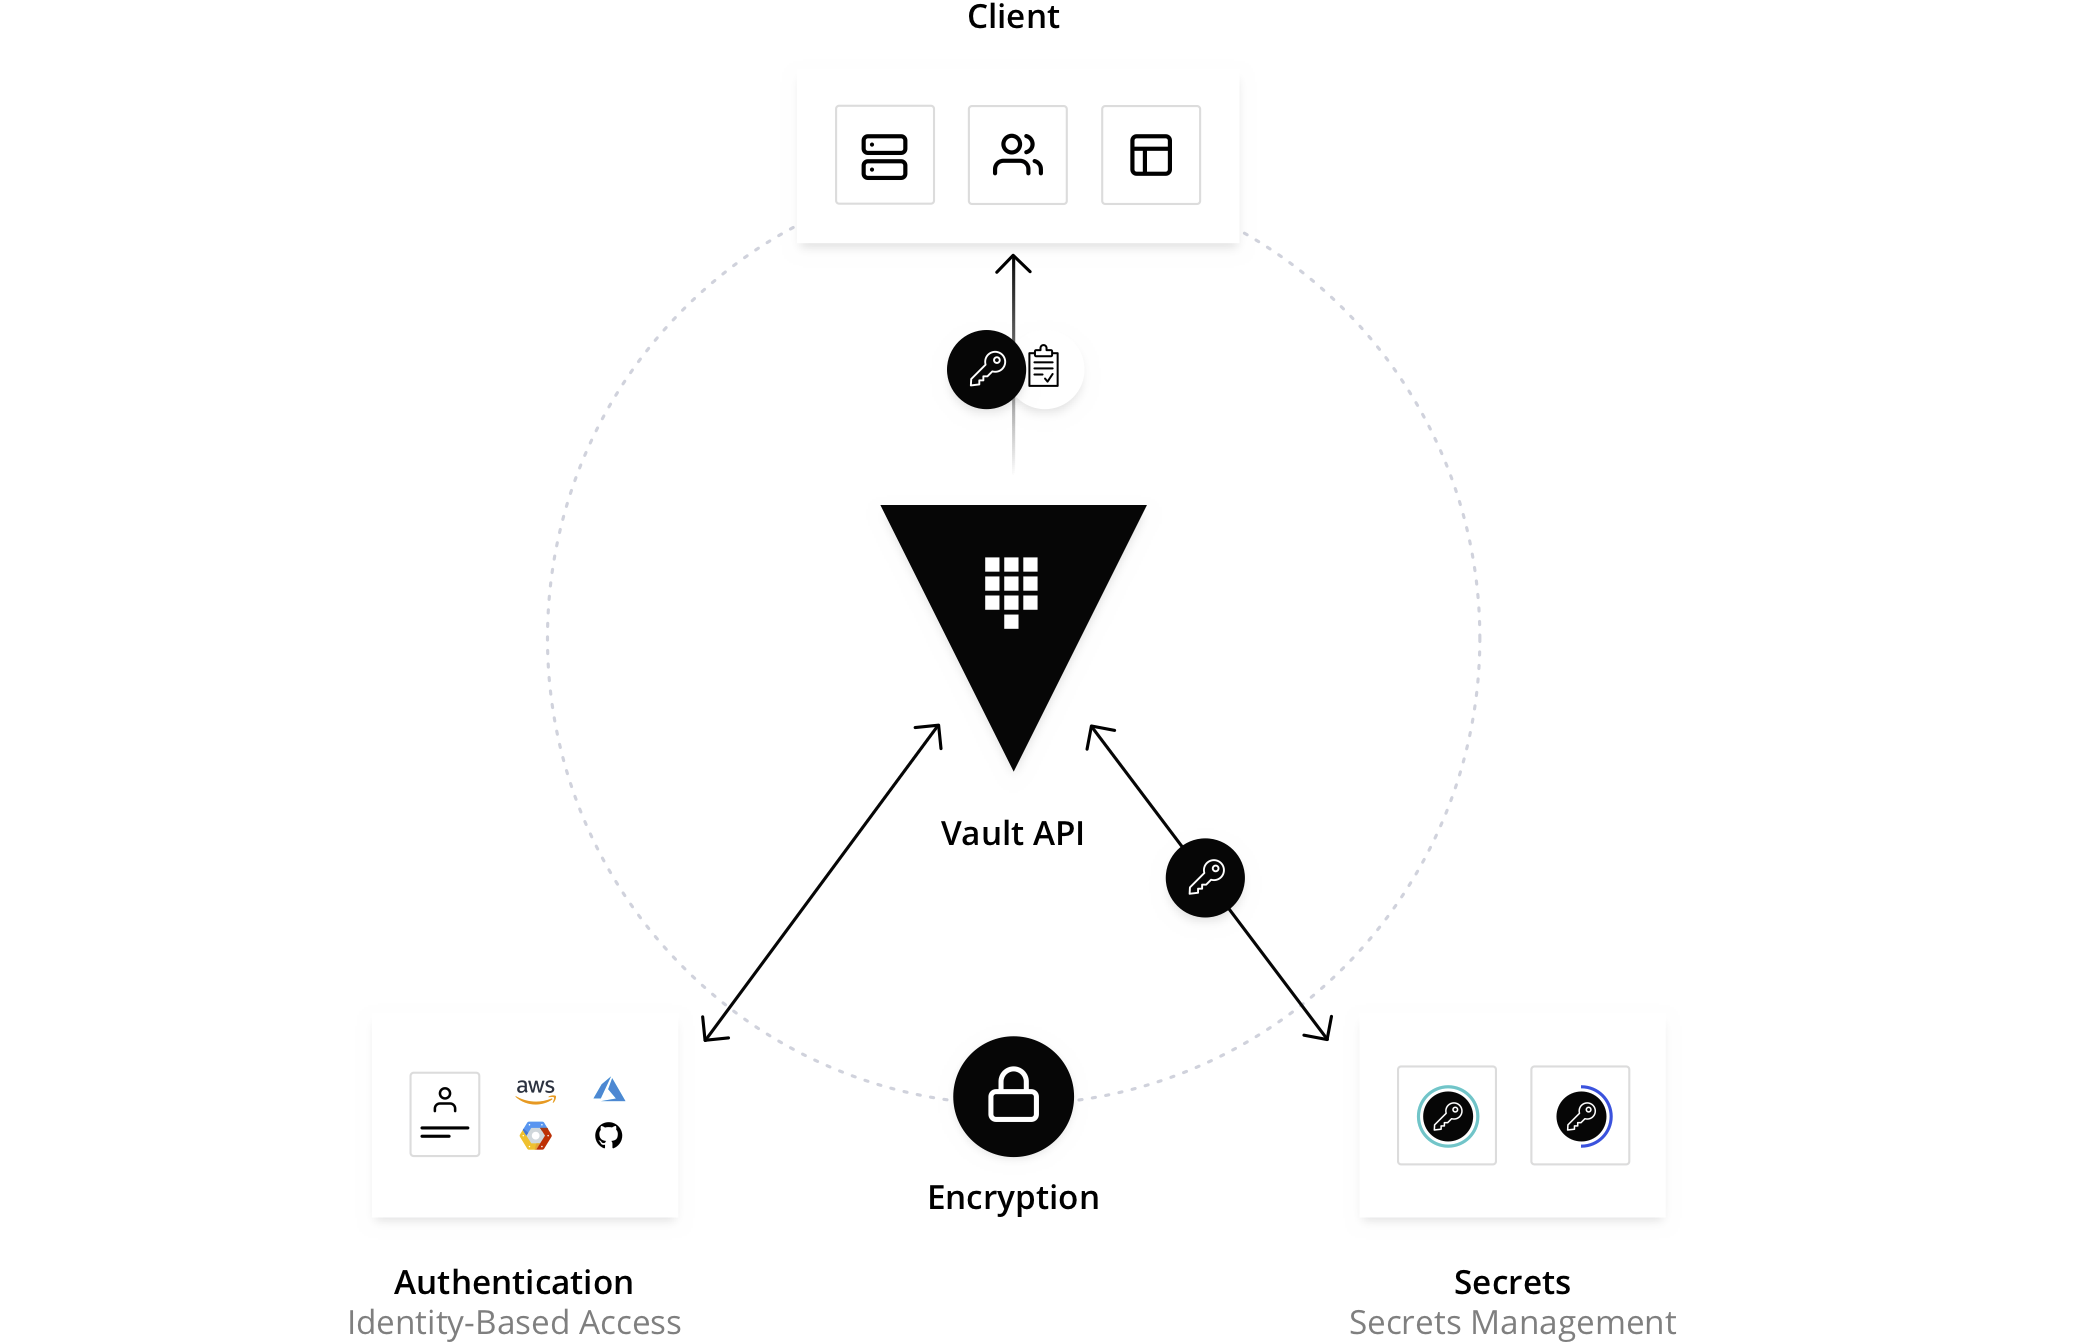
\includegraphics[scale=0.2]{tesi/files/immagini/vault_schema.png}
    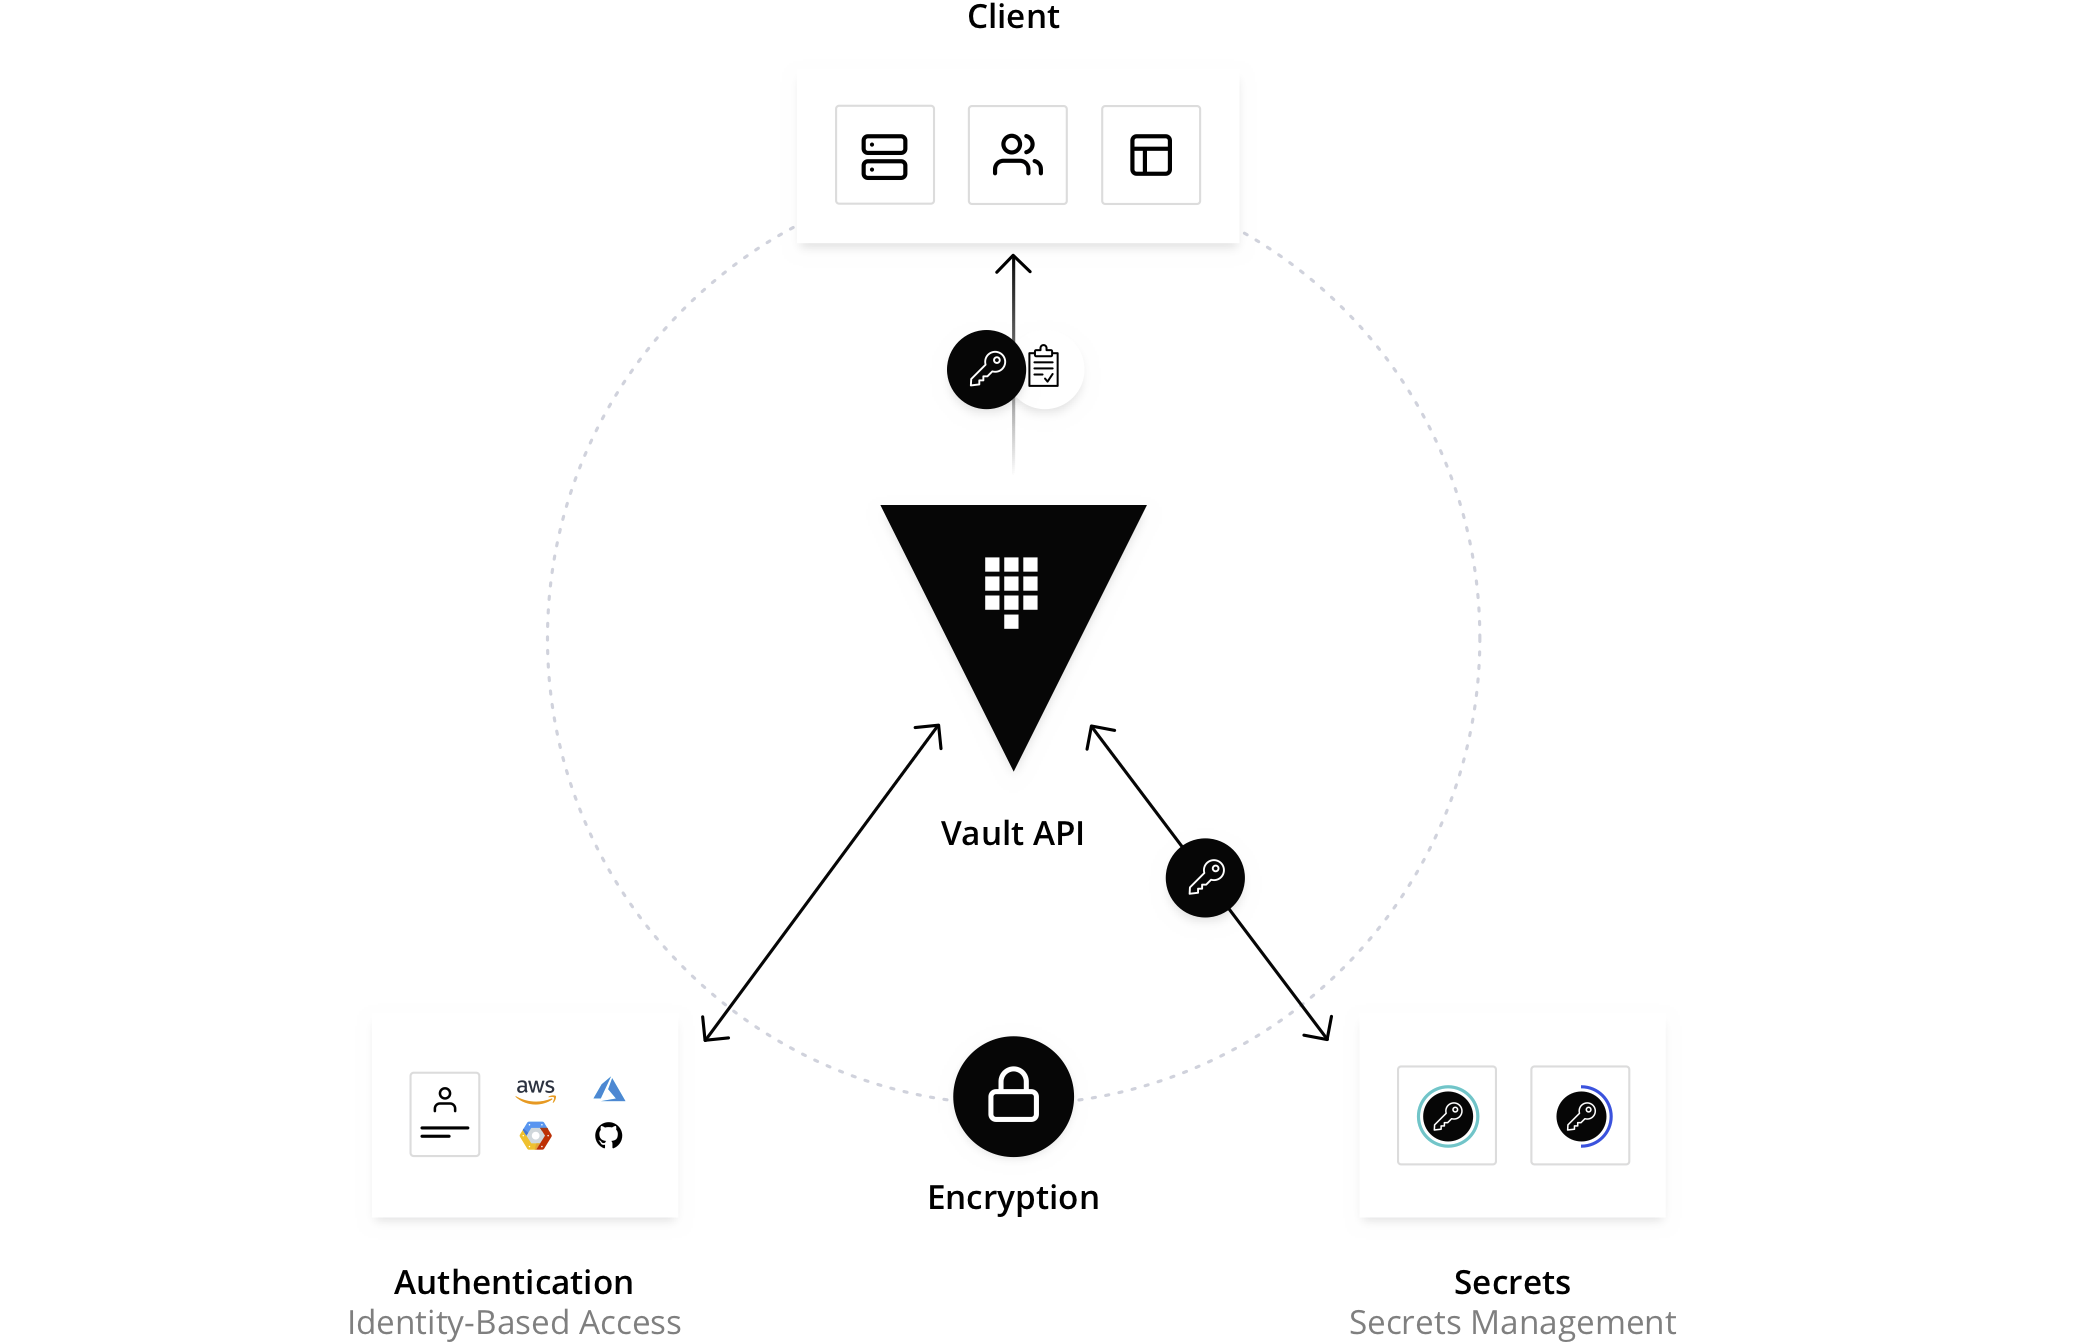
\includegraphics[width=0.9\linewidth]{tesi/files/immagini/vault_schema.png}
    %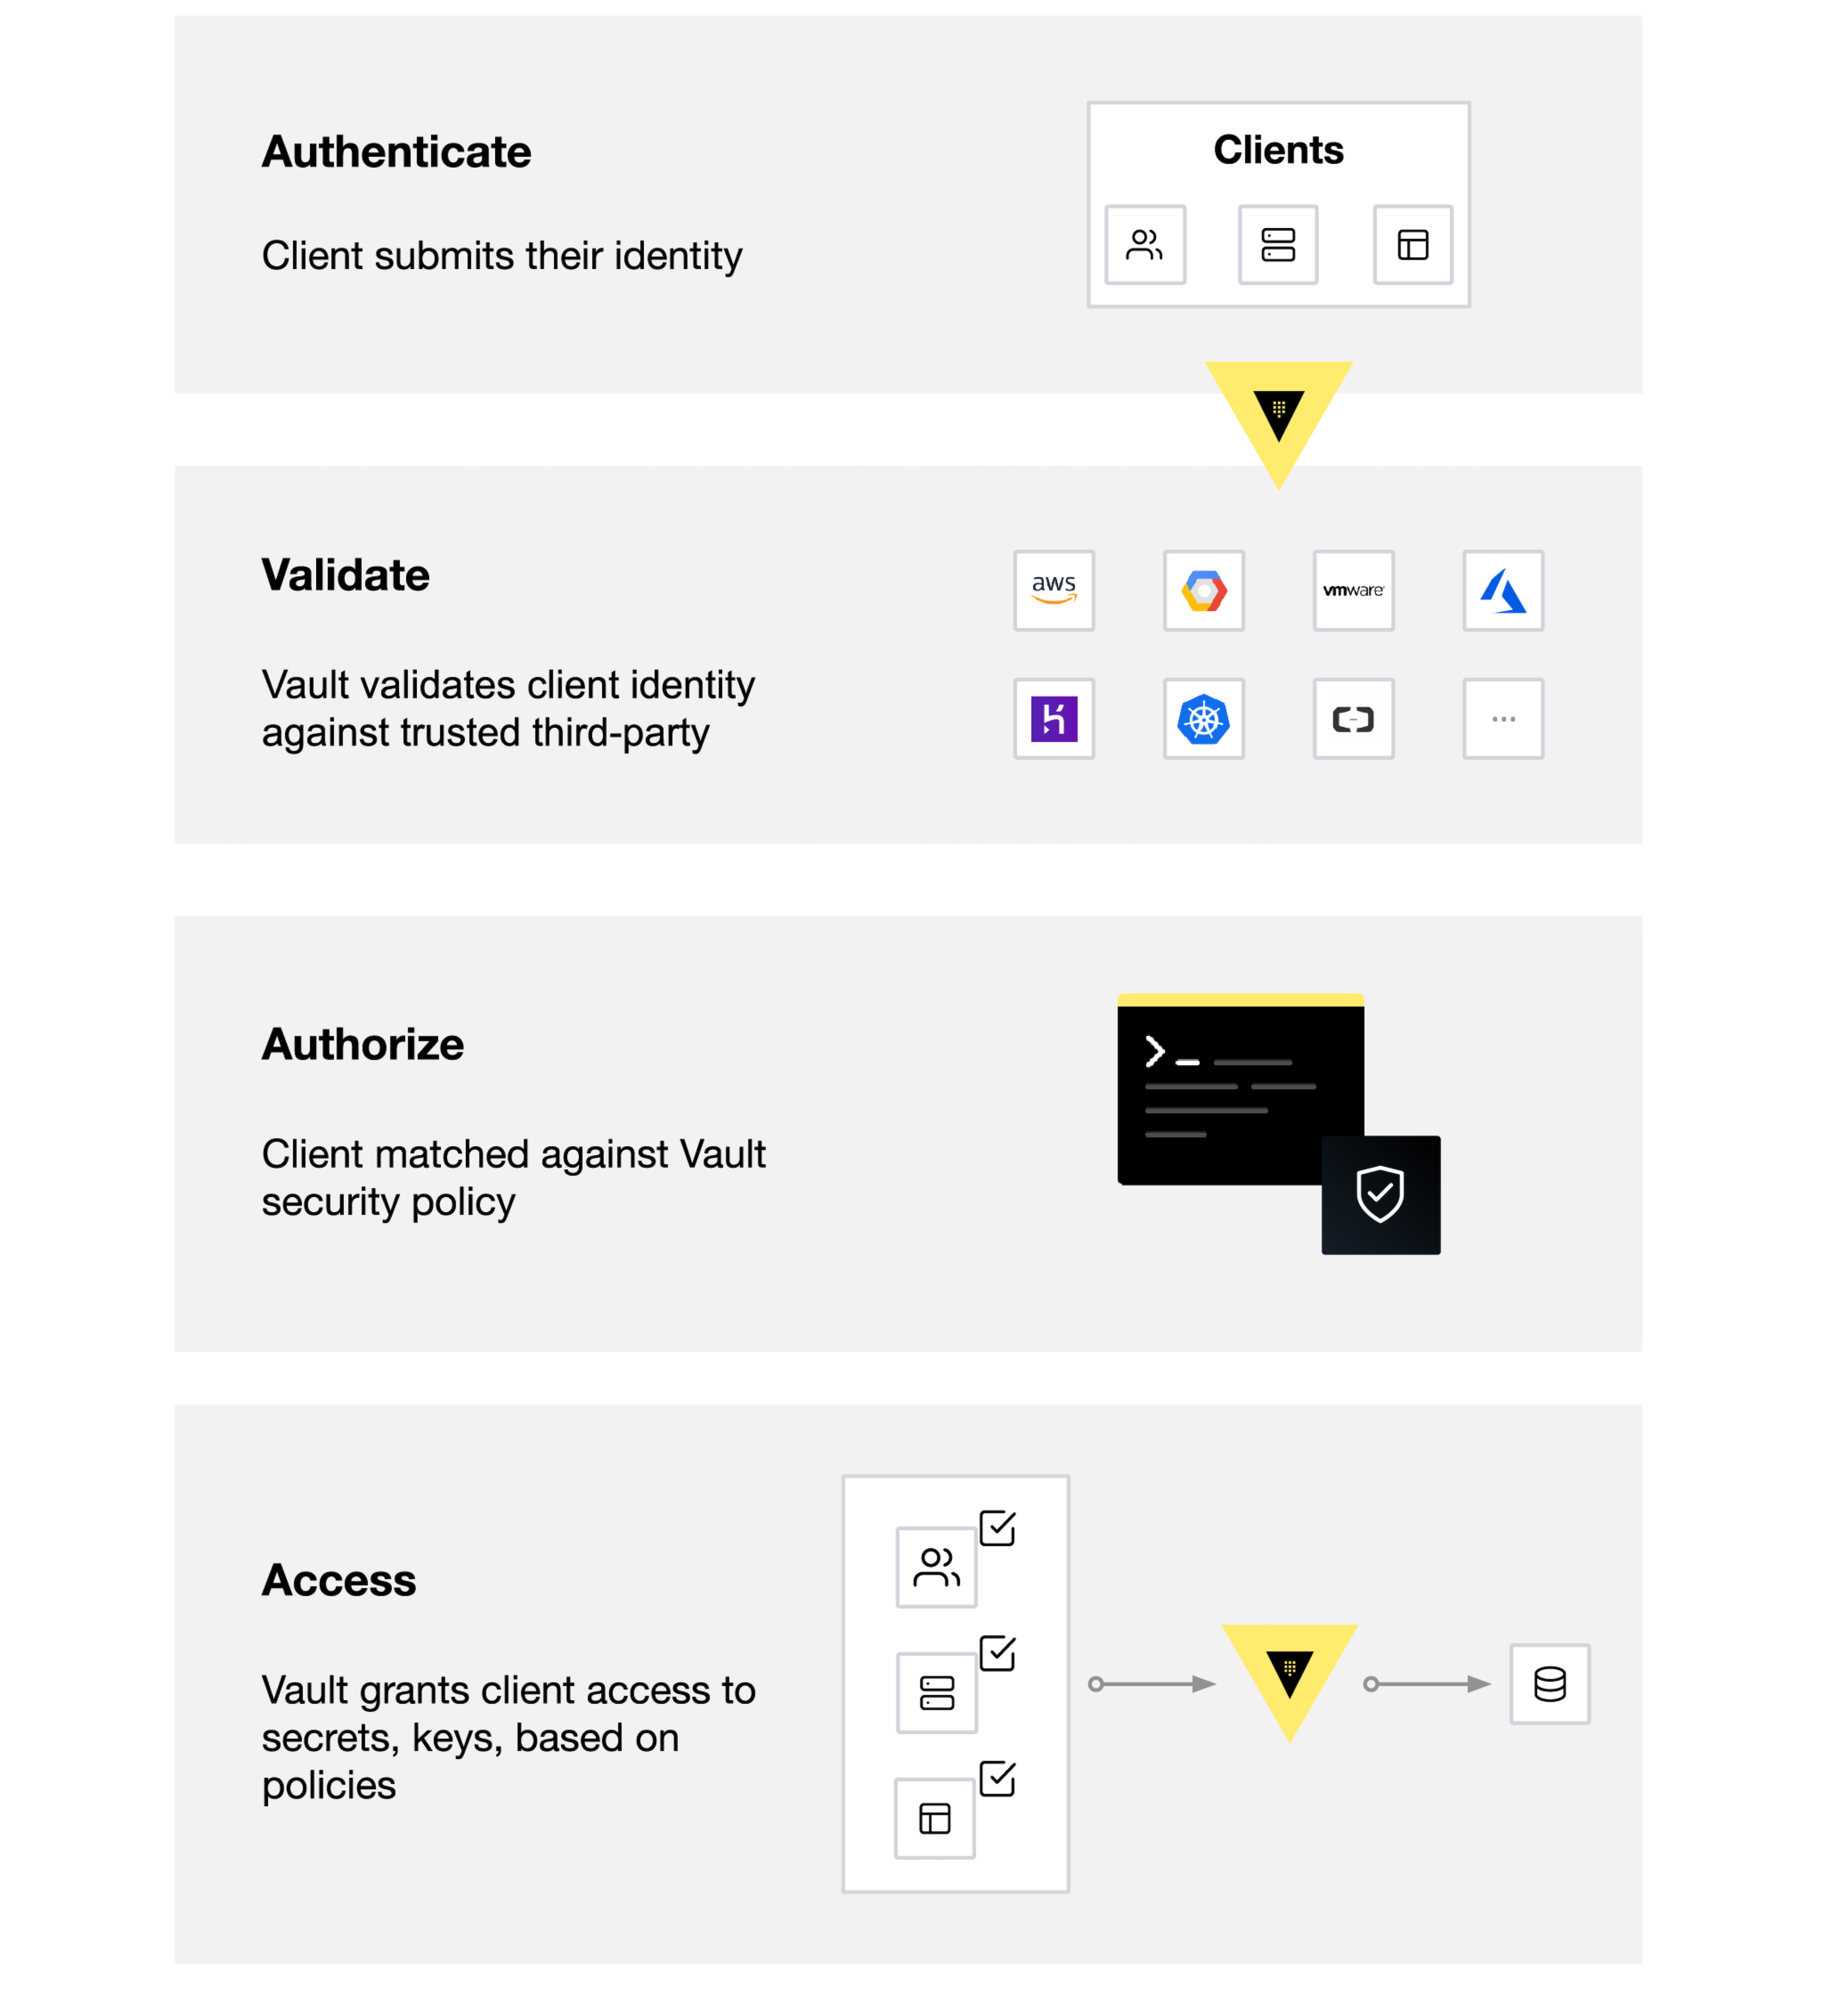
\includegraphics[scale=0.04]{tesi/files/immagini/vault_schema_2.png}
    \caption{Schema di funzionamento di Vault \cite{vault_home}.}
    \label{fig:vault_schema}
\end{figure}

In figura \ref{fig:vault_schema} è schematizzato il funzionamento di Vault. La prima cosa che ciascun client deve fare è autenticarsi e, durante questa procedura, Vault verifica l'identità attraverso il provider di autenticazione che è stato configurato. Una volta autenticato, il client può richiedere uno specifico \textit{secret} e, una volta verificato che il suddetto client abbia le autorizzazioni necessarie, Vault restituisce il \textit{secret} richiesto.

Come detto in precedenza, Vault verifica l'identità degli utenti tramite un provider di autenticazione. Sono disponibili numerosi provider che permettono di interfacciarsi con altrettanti servizi esterni (e.g. AWS, Azure, GitHub, Google Cloud, LDAP, Username e Password, ecc.), in questo modo si ha una vasta flessibilità. Il charm di Vault utilizza di default il provider basato sui Token \cite{vault_documentation}.

\subsection{Open vSwitch e Open Virtual Network}
\label{subsubsec:ovs} 

\paragraph{Open vSwitch.}Open vSwitch (OvS) è un software open source che implementa uno switch virtuale. È progettato in modo da permettere un'ampia automazione della rete mantenendo al contempo il supporto a interfacce e protocolli di gestione standard. Supporta inoltre l'installazione distribuita su più macchine fisiche \cite{ovs_home}.

\paragraph{Open Virtual Network.} Open Virtual Network (OVN) consiste in una serie di demoni che si appoggiano a Open vSwitch e implementano i layer di astrazione più alti; OVN permette infatti lavorare con router e switch logici ed è studiato per essere usato dai cloud management software (OpenStack nel nostro caso). Alcune delle sue funzionalità più rilevanti sono: router virtuali distribuiti, switch virtuali distribuiti, Access Control Lists (ACL), DHCP e DNS server \cite{ovn_home}.

\subsection{Ceph}\label{sec:ceph}
Ceph è una piattaforma open source di software-defined storage, ovvero una piattaforma software che gestisce l'archiviazione dei dati in modo indipendente dall'hardware sottostante. Una sua caratteristica fondamentale è che supporta i cosiddetti \textit{storage cluster}, che consistono nell'aggregazione di più host fisici (potenzialmente anche migliaia) in un volume di storage unico che viene poi gestito da Ceph stesso in modo che i client non debbano preoccuparsi della posizione in cui archiviare o reperire i dati \cite{ceph_documentation}.

Ciascun \textit{storage cluster} è composto da diversi componenti software:
\begin{itemize}
    \item Ceph OSD Daemon (OSD): è il demone che interagisce con i volumi di storage su ciascuna macchina che compone il cluster e si occupa dell'immagazzinamento dei dati
    \item Ceph Monitor (MON): mantiene una copia della mappa dell'intero cluster
    \item Ceph Manager: funziona insieme a Ceph Monitor e il suo compito è quello di interfacciarsi con sistemi di monitoraggio esterni (non è fondamentale per il funzionamento del cluster)
\end{itemize}

Ceph mette a disposizione 3 modalità di storage in un unico sistema: object storage, block storage e file storage.

\paragraph{Object storage.} L'object storage è un formato di storage nel quale i dati vengono archiviati in unità separate chiamati oggetti. Ciascuno di questi oggetti possiede una chiave univoca che ne permette l'individuazione all'interno di un sistema distribuito.

\paragraph{Block storage.} Il block storage è un formato di storage nel quale i dati vengono suddivisi in componenti di dimensione fissa detti blocchi, ciascuno dei quali dotato di un id univoco. Questo id, in modo analogo a quello che succede nell'obecjt storage, permette di individuare un singolo blocco all'interno di un sistema distribuito.

\paragraph{File storage.} Il file storage è il formato di storage più conosciuto: i dati vengono archiviati in una struttura gerarchica di directory. Questo è il sistema che viene utilizzato ad esempio sui computer o sui NAS \cite{storage_formats_description}.
\newpage

\chapter{Installazione di OpenStack}
% https://docs.openstack.org/charm-guide/latest/index.html
% https://docs.openstack.org/charm-guide/latest/concepts/charm-types.html
Una volta creato il model con Juju (ref), che rappresenta il contenuto software del cloud, arriva il momento di popolarlo con le applicazioni che costituiranno i servizi del cloud.
% 
Per fare ciò si utilizza sempre Juju, il quale in maniera più o meno automatizzata effettuerà il deployment dei charm sui vari nodi indicati.

Prima di procedere nell'installazione, è importate prestare attenzione ad alcuni aspetti, in particolare quelli riguardanti le versioni, in quanto essendo un progetto in rapido sviluppo le versioni utilizzate in questo documento diverranno con molta probabilità obsolete nel giro di una manciata di mesi.


\section{Concetti preinstallazione}
\subsection{Tipologie di charm su OpenStack.} 
Su OpenStack esistono due tipologie di charm \cite{openstack_charms_type}: quelli che utilizzano i \emph{channel} e quelli \emph{legacy} che non lo utilizzano.

I charm di tipo \textbf{channel} sono quelli la cui release è dedicata ad una specifica combinazione del sistema operativo (detta anche \emph{series}) e della versione di OpenStack;
% 
questa combinazione è chiamata \emph{series-openstack}
% 
Questo implica che se un charm funziona per una recente combinazione di series-openstack, non è garantito che funzioni correttamente su una combinazione precedente.
% 
Inoltre, bisogna passare ad un channel diverso nel caso in cui si voglia eseguire l'aggiornamento ad una nuova versione di OpenStack. 
% 
Per fare un esempio, durante il deploy di alcuni charm si è utilizzato l'argomento \code{-{}-channel yoga/stable}; ciò implica la versione di OpenStack Yoga, che è funzionante sulla versione di Ubuntu Focal (20.04 LTS) o Jammy (22.04 LTS).

I charm di tipo \textbf{legacy} invece includono all'interno tutte le funzionalità delle revisioni precedenti e dunque funzionano anche con una combinazione series-openstack antecedente.
% 
Tuttavia, il loro sviluppo si è fermato dalla versione 21.10 di OpenStack Charms (Ottobre 2021), di conseguenza l'ultimo supporto alla combinazione series-openstack è quella \code{focal-xena}.

In questo progetto sono stati utilizzati solo charms di tipo channel, e su ogni comando di deploy è stata specificata appunto la versione.
% 
In caso si volessero replicare i comandi su series-openstack più aggiornati, è necessario consultare le versioni adeguate dei channel nelle pagine di documentazione individuali dei singoli charm.



\subsection{Versione di OpenStack.}\label{sec:openstack_version} 
All'inizio del progetto di questa tesi, era da poco uscita la versione di OpenStack chiamata \emph{Yoga}, in data 2022-03-30, e pertanto tutta l'installazione è basata su questa versione.
% 
Durante la conclusione dei lavori progettuali, in data 2022-10-05 è uscita una nuova release, chiamata \emph{Zed} , mentre nel prossimo futuro è prevista l'uscita di \emph{Antelope} con data stimata 2023-03-22, e la successiva versione \emph{Bobcat} con data stimata 2023-10-04.
%
Nonostante il progetto OpenStack cresca velocemente, le release vengono mantenute a lungo, anche grazie al supporto della community;
% 
per esempio, la versione \emph{Queens} uscita in data 2018-02-28 ha terminato solo da poco il suo ciclo di vita (2023-01-18), avendo 
quindi potuto godere di un supporto per quasi cinque anni.



\subsection{Distribuzione dei charm all'interno delle macchine del cluster.}
Come spiegato nella \cref{subsec:juju_funzionamento}, è compito di Juju di occuparsi del completo dispiegamento delle applicazioni nelle varie macchine collegate su MAAS.
% 
Le varie applicazioni saranno distribuite tra le quattro macchine a disposizione, in modo tale da avere una ripartizione equa in termini di risorse computazionali e di storage.
% 
In oltre, alcune di esse verranno replicate su più macchine in modo tale da creare ridondanza e suddivisione del carico di lavoro.
% 
Quindi, tutti gli aspetti inerenti al ciclo di vita delle applicazioni come l'installazione o la sincronizzazione tra le unit (le istanze effettive in esecuzione delle applicazioni), saranno gestiti completamente da Juju.
% 
Le uniche cose necessarie da definire sono quali charm installare e la loro versione, su quale macchine dispiegarli e risolvere le loro relazioni (integrazioni dalla versione 3.0 di Juju).

La decisione su quali charm usare e la loro suddivisione adottata in questo progetto è quella implementata da Canonical nei suoi esempi di Charms Deployment (\cref{sec:deplyoment_method}).
% 
Di seguito vengono elencate le applicazioni e i relativi charm suddivisi tra le quattro macchine (la quinta è stata successivamente utilizzata per il deployment dei servizi dedicati al load balancer).

% \footnotesize
\begin{itemize}
    \footnotesize
    \item Ceph OSD (\code{ceph-osd}), OVN Central (\code{ovn-central}), MySQL InnoDB Cluster (\code{mysql-innodb-cluster}), Keystone (\code{keystone}), Ceph Mon (\code{ceph-mon}) e Ceph RADOS Gateway (\code{ceph-radogsw}).

    \item Ceph OSD (\code{ceph-osd}), Nova Compute (\code{nova-compute}), MySQL InnoDB Cluster (\code{mysql-innodb-cluster}), OVN Central (\code{ovn-central}), Cinder (\code{cinder}), Neutron API (\code{neutron-api}), Ceph Mon (\code{ceph-mon}).

    \item Ceph OSD (\code{ceph-osd}), Nova Compute (\code{nova-compute}), MySQL InnoDB Cluster (\code{mysql-innodb-cluster}), OVN Central (\code{ovn-central}), RabbitMQ Server (\code{rabbitmq-server}), OpenStack Dashboard (\code{openstack-dashboard}), Ceph Mon (\code{ceph-mon}).

    \item Ceph OSD (\code{ceph-osd}), Nova Compute (\code{nova-compute}), Nova Cloud Controller (\code{nova-cloud-controller}), Vault (\code{vault}), Glance (\code{glance}).
\end{itemize}


% \noindent
% OPPURE

% \begin{enumerate}
%     \item Ceph OSD, MySQL InnoDB Cluster, OVN Central, Keystone, Ceph Mon e Ceph RADOS Gateway.
    
%     \item Ceph OSD, Nova Compute, MySQL InnoDB Cluster, OVN Central, Neutron API, Ceph Mon, Cinder.

%     \item Ceph OSD, Nova Compute, MySQL InnoDB Cluster, OVN Central, RabbitMQ Server, OpenStack Dashboard, Ceph Mon.

%     \item Ceph OSD, Nova Compute, Vault, Nova Cloud Controller , Placement, Glance.
% \end{enumerate}
    
% \begin{enumerate}
%     \item ceph-osd, mysql-innodb-cluster, ovn-central (neutron), keystone, ceph-mon, ceph-radogsw

%     \item ceph-osd, nova-compute, mysql-innodb-cluster, ovn-central (neutron), neutron-api, ceph-mon, cinder

%     \item ceph-osd, nova-compute, mysql-innodb-cluster, ovn-central (neutron), rabbitmq-server, openstack-dashboard, ceph-mon

%     \item ceph-osd, nova-compute, vault, nova-cloud-controller, placement, glance 
% \end{enumerate}
    
\subsection{Monitoraggio del deploy.}
Indipendentemente dalla tipologia di deployment scelta (un charm alla volta o in bundle rif), è possibile seguire ogni singolo passaggio che Juju effettua all'interno del cluster.
% 
Eseguendo il comando \code{juju status} quindi, verrà stampato lo stato attuale del cloud, elencando per ogni applicazione, unit e relazione varie informazioni a riguardo, come la macchina o il container sul quale verranno installati, i vari indirizzi IP e lo status ognuno di essi.

\begin{figure}[H]
    \centering
    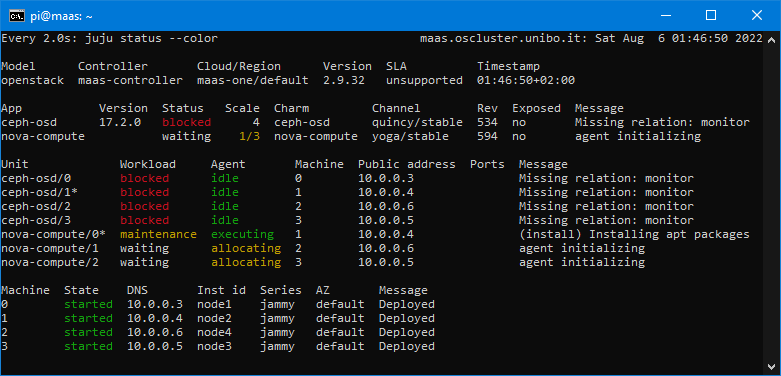
\includegraphics[width=1\linewidth]{tesi/files/immagini/openstack/es_juju_status.png}
    \caption{Esempio d'output di \code{juju status} durante le prime fasi di deploy dei charm.}
    \label{fig:openstack_es_status}
\end{figure}

\bigskip\noindent
In particolare, è molto utile specialmente le prime volte per capire ed imparare i vari status delle applicazioni, nonché come primo punto di debug in caso di anomalie; 
% 
questo perché verranno mostrati anche messaggi sulla condizione di ogni elemento mostrato, come è possibile vedere in \cref{fig:openstack_es_status}.

Durante tutto il deployment del cloud, sarà normale notare messaggi come relazioni mancanti o unit bloccate, in quanto tali requisiti non possono essere risolti immediatamente fintanto che una successiva applicazione non viene installata.
% 
Un modo più conveniente per monitorare la progressione del deploy è quello di eseguire il comando \code{watch -n 5 -c juju status -{}-color} in un terminale separato; 
% 
questo comando eseguirà ogni \code{5} secondi il comando \code{juju status -{}-color}, molto utile per avere un continuo aggiornamento sull'avanzamento dell'installazione.


\newpage

\section{Installazione manuale}\label{sec:openstack_manual_installation}
In questa sezione verrà effettuato il deploy del cloud OpenStack installando un charm alla volta.
% 
Tuttavia, Juju si occuperà dell'installazione ed effettiva configurazione di ogni singolo componente.
% 
L'intero processo di installazione richiede non poco tempo, e a seconda della velocità delle macchine e del tempo impiegato dall'operatore possono occorrere all'incirca 30/60 minuti per un'installazione veloce fino a 120/180 minuti per un'installazione più analitica.
% 
Per maggiori dettagli, si rimanda alla documentazione \cite{openstack_installation_juju}.

Come prima cosa, bisogna assicurarsi che i comandi verranno impartiti al Juju controller e al model corretto (\cref{sec:juju_model_create}).
% 
Per farlo, baserà eseguire il comando mostrato nel \cref{lst:openstack_install_switch}.

% \begin{minipage}{0.96\linewidth} 
\begin{lstlisting}[
    language=mybash, 
    caption={Comando per selezionare il Juju controller e il corretto model.}, 
    label={lst:openstack_install_switch},
]
juju switch maas-controller:openstack
\end{lstlisting}
% \end{minipage}

\bigskip\noindent
Ora è possibile effettuare i deploy dei vari charm;
% 
tra l'esecuzione di un comando e l'altro non è necessario aspettare che Juju finisca nei vari procedimenti.
% 
Tuttavia, specialmente le prime volte, è consigliato eseguire un comando alla volta per apprendere al meglio le varie fasi di deploy.



 \bigskip\noindent
% \hfill\break
\paragraph{Ceph OSD.}
Il primo charm che si andrà ad installare è quello inerente al gestore d'archiviazione dei dati, ceph-osd (\cref{sec:ceph}).
% 
Questo charm bisogna configurarlo il maniera corretta, indicandogli dispositivi di storage da utilizzare.
% 
in questo progetto tutti i nodi montano gli stessi dispositivi di storage.

Per configurare i charm in maniera agile, si utilizzano i file di configurazione \code{YAML};
% 
quindi è stato creato il file \code{ceph-osd.yaml} con le configurazioni mostrate nel \cref{lst:openstack_install_ceph-osd.yaml}.

% \begin{minipage}{0.96\linewidth} 
\begin{lstlisting}[
    language=yaml, 
    caption={Configurazione di \emph{ceph-osd} nel file \emph{ceph-sod.yaml}.}, 
    label={lst:openstack_install_ceph-osd.yaml},
]
ceph-osd:
  osd-devices: /dev/sda /dev/sdb
  source: distro
\end{lstlisting}
% \end{minipage}

\bigskip\noindent
Il charm ceph-osd verrà installato su tutti e 4 i nodi;
% 
essendo il primo deploy, sui nodi non è ancora presente il sistema operativo, quindi durante questa fase verrà installato anche quest'ultimo in maniera automatica, applicando le immagini scaricate attraverso MAAS.
% 
nel \cref{lst:openstack_install_ceph-osd} viene mostrato il comando per il deploy di ceph-osd.
% \begin{minipage}{0.96\linewidth} 
\begin{lstlisting}[
    language=mybash, 
    caption={Deploy del charm \emph{ceph-osd}.}, 
    label={lst:openstack_install_ceph-osd},
]
juju deploy -n 4 --series jammy --channel quincy/stable --config ceph-osd.yaml --constraints tags=compute ceph-osd
\end{lstlisting}
% \end{minipage}
\begin{itemize}
    \item Con \code{-n} viene indicato su quanti nodi effettuare il deploy del charm, in questo caso su tutti e quattro i nodi.
    
    \item Con \code{-{}-series} e con \code{-{}-channel} viene indicato di fatto la versione del sistema operativo e del charm.

    \item Con \code{-{}-config} è possibile specificare il file \code{YAML} per applicare delle configurazioni personalizzate.

    \item  Con \code{-{}-constraints} è possibile specificare in maniera accurata i requisiti  hardware per le nuove macchine su cui effettuare il deploy.
    % 
    Questi requisiti possono essere ad esempio memoria ram, tag, space, etc.
    % 
    In questo caso specifico è stato indicato di effettuare il deploy su tutti i nodi aventi il tag \emph{compute} (impostato durante le fasi di add dei nodi su MAAS nella \cref{itm:tag_node} della \cref{subsubsec:maas_add_node}).
\end{itemize}



% \bigskip
\paragraph{Nova Compute.}
Il prossimo charm da installare è nova-compute (\cref{sec:openstack_nova}), usato per gestire le macchine virtuali.
% 
Anche in questo caso l'installazione del charm sarà personalizzata con l'inserimento di qualche impostazione salvata nel file \code{nova-compute.yaml}, contenente le configurazioni mostrate nel \cref{lst:openstack_install_nova-compute.yaml}.
% \begin{minipage}{0.96\linewidth} 
\begin{lstlisting}[
    language=yaml, 
   caption={Configurazione di \emph{nova-compute} nel file \emph{nova-compute.yaml}.},
    label={lst:openstack_install_nova-compute.yaml},
]
nova-compute:
  config-flags: default_ephemeral_format=ext4
  enable-live-migration: true
  enable-resize: true
  migration-auth-type: ssh
  virt-type: qemu
  openstack-origin: distro
\end{lstlisting}
% \end{minipage}

\bigskip\noindent
Quindi è possibile effettuare il deploy del charm nova-compute su tre macchine.
% \begin{minipage}{0.96\linewidth} 
\begin{lstlisting}[
    language=mybash, 
   caption={Deploy del charm \emph{nova-compute}.},
    label={lst:openstack_install_nova-compute},
]
juju deploy -n 3 --to 1,2,3 --series jammy --channel yoga/stable --config nova-compute.yaml nova-compute
\end{lstlisting}
% \end{minipage}
\begin{itemize}
    \item Con \code{-{}-to} è possibile indicare in maniera precisa su quali macchine andare ad effettuare i deploy del charm.
    % 
    Queste macchine devono essere già state aggiunte in Juju, e in questo caso è avvenuto con il primo comando di deploy.
    % 
    Il numero indicato rappresenta l'indice della macchina, ed è possibile prenderne nota attraverso il comando \code{juju status}.   
\end{itemize}


% \bigskip
\paragraph{MySQL InnoDB Cluster.}
Il charm che si occuperà della creazione e gestione del database per archiviare tutte le varie informazioni che gli altri charm utilizzeranno è mysql-innodb-cluster.
% 
Questo charm richiede sempre almeno tre unit, e saranno containerizzate tramite LXD nelle macchine 0, 1 e 2.
% \begin{minipage}{0.96\linewidth} 
\begin{lstlisting}[
    language=mybash, 
   caption={Deploy del charm \emph{mysq-innodb-cluster}.},
    label={lst:openstack_install_mysq-innodb-cluster},
]
juju deploy -n 3 --to lxd:0,lxd:1,lxd:2 --series jammy --channel 8.0/stable mysql-innodb-cluster
\end{lstlisting}
% \end{minipage}



% \bigskip
\paragraph{Vault.}
In questa fase verrà installato il charm vault (\cref{sec:vault}) in una unica unit, il quale gestirà tutte quelle informazioni sensibili denominate come \emph{secret}, come ad esempio i certificati TLS per la comunicazione crittografata tra le applicazioni cloud.
% \begin{minipage}{0.96\linewidth} 
\begin{lstlisting}[
    language=mybash, 
   caption={Deploy del charm \emph{vault}.},
    label={lst:openstack_install_vault},
]
juju deploy --to lxd:3 --series jammy --channel 1.7/stable vault
\end{lstlisting}
% \end{minipage}

\bigskip\noindent
Questo charm deve essere messa in relazione con il database del cloud.
% 
Per farlo, è necessario installare una unit specifica del subordinate \emph{mysql-router}, che si comporterà da tramite tra vault e mysql-innodb-cluster.
% 
Una volta installato, è possibile aggiungere le relazioni come mostrato in \cref{lst:openstack_install_vault_rel}.
% \begin{minipage}{0.96\linewidth} 
\begin{lstlisting}[
    language=mybash, 
   caption={Deploy del subordinate \emph{mysql-router} per le relazioni con vault.},
    label={lst:openstack_install_vault_rel},
]
juju deploy --channel 8.0/stable mysql-router vault-mysql-router
juju add-relation vault-mysql-router:db-router mysql-innodb-cluster:db-router
juju add-relation vault-mysql-router:shared-db vault:shared-db
\end{lstlisting}
% \end{minipage}


\subparagraph{Configurazione di vault.}\label{subpar:vault_configuration}
Finita l'installazione di vault, è necessario inizializzarlo e "aprirlo".
% 
Innanzitutto bisogna installare il client Vault attraverso snap.
% \begin{minipage}{0.96\linewidth} 
\begin{lstlisting}[
    language=mybash, 
   caption={Installazione del client \emph{Vault}.},
    label={lst:openstack_install_vault_install},
]
sudo snap install vault
\end{lstlisting}
% \end{minipage}

\bigskip\noindent
Successivamente, si estrapola l'indirizzo IP del container sul quale è stato installato; 
% 
l'indirizzo IP è possibile visionarlo anche attraverso \code{juju status}.
% 
L'indirizzo IP serve per inizializzare la variabile \code{VAULT\_ADDR} con l'URI del charm vault, necessaria per le fasi successive.
% \begin{minipage}{0.96\linewidth} 
\begin{lstlisting}[
    language=mybash, 
   caption={Crezione della variabile d'ambiente \code{VAULT\_ADDR}.},
    label={lst:openstack_install_vault-ip},
]
IP_VAULT=$(juju status --format=yaml vault | grep public-address | awk '{print $2}' | head -1)
export VAULT_ADDR="http://${IP_VAULT}:8200"
\end{lstlisting}
% \end{minipage}

\bigskip\noindent
A questo punto è possibile inizializzare Vault, indicandogli di creare cinque chiavi e di necessitarne tre per la sua apertura.
% 
Queste chiavi poi sono state esportate sul file \code{vault-keys} per una miglior comprensione ed utilizzo.
% 
Queste chiavi sono salvate in chiaro, ed è consigliato conservarle in un luogo sicuro.
% \begin{minipage}{0.96\linewidth} 
\begin{lstlisting}[
    language=mybash, 
   caption={Generazione delle chiavi d'apertua del vault.},
    label={lst:openstack_install_vault_keygen},
]
vault operator init -key-shares=5 -key-threshold=3 > vault-keys
\end{lstlisting}
% \end{minipage}

\bigskip\noindent
Ora è possibile aprire Vault, utilizzando tre delle cinque chiavi generate nel \cref{lst:openstack_install_vault_keygen}.
% \begin{minipage}{0.96\linewidth} 
\begin{lstlisting}[
    language=mybash, 
   caption={Unseal del client Vault.},
    label={lst:openstack_install_vault_unseal},
]
vault operator unseal <key1>
vault operator unseal <key2>
vault operator unseal <key3>
\end{lstlisting}
% \end{minipage}
\begin{itemize}
    \item Al posto di \code{<key1>}, \code{<key2>} e \code{<key3>}, bisogna inserire tre chiavi a piacere tra le cinque a disposizione. 
\end{itemize}

\bigskip\noindent
Una volta aperto il client Vault, bisogna autorizzare il charm vault a poter interagire con esso e creare e gestire i secret.
% 
Per farlo, viene creato un token root dalla durata di 10 minuti.
% \begin{minipage}{0.96\linewidth} 
\begin{lstlisting}[
    language=mybash, 
   caption={Generazione del token temporaneo.},
    label={lst:openstack_install_vault_tokengen},
]
export VAULT_TOKEN=<Initial Root Token>
vault token create -ttl=10m
\end{lstlisting}
% \end{minipage}
\begin{itemize}
    \item Il \code{<Initial Root Token>} è possibile trovarlo nell'output (nel file se è stato salvato) del \cref{lst:openstack_install_vault_keygen}.
\end{itemize}

\bigskip\noindent
Infine, è possibile autorizzare il charm vault con il token appena generato nel \cref{lst:openstack_install_vault_tokengen}.
% 
Con il comando \code{run-action}, è possibile far eseguire ai charm un'azione tra quelle che concedono, in base all'implementazione del charm stesso.
% \begin{minipage}{0.96\linewidth} 
\begin{lstlisting}[
    language=mybash, 
   caption={Autorizzazione al charm \emph{vault}.},
    label={lst:openstack_install_vault_authorise},
]
juju run-action --wait vault/leader authorize-charm token=<token>
\end{lstlisting}
% \end{minipage}
\begin{itemize}
    \item Al posto di \code{<token>} bisogna inserire il token temporaneo generato nel \cref{lst:openstack_install_vault_tokengen}.
\end{itemize}


\bigskip\noindent
A charm autorizzato, è possibile creare un certificato autofirmato se non se ne possiede uno rilasciato da una CA.
% \begin{minipage}{0.96\linewidth} 
\begin{lstlisting}[
    language=mybash, 
   caption={Creazione del certificato autofirmato.},
    label={lst:openstack_install_vault_self-crt},
]
juju run-action --wait vault/leader generate-root-ca > vault-ca.crt
\end{lstlisting}
% \end{minipage}


\bigskip\noindent
Come ultimo passaggio, verrà collegato il certificato di vault, creato nel \cref{lst:openstack_install_vault_self-crt}, al DB del cloud attraverso l'aggiunta della relativa relazione.
% \begin{minipage}{0.96\linewidth} 
\begin{lstlisting}[
    language=mybash, 
   caption={Aggiunta della relazione per collegare il certificato a DB.},
    label={lst:openstack_install_vault_add_crt},
]
juju add-relation mysql-innodb-cluster:certificates vault:certificates
\end{lstlisting}
% \end{minipage}



\paragraph{Neutron.}
Per implementare la rete con Neutron (\cref{sec:openstack_neutron}), verranno installati quattro charms:
% 
\begin{itemize}
    \item ovn-central per il controllo delle OVN (\cref{subsubsec:ovs}), installato su tre unit.
    \item neutron-api fornisce il servizio di API di Neutron, installato in una unica unit.
    \item neutron-api-plugin-ovn subordinate di neutron-api.
    \item ovn-chassis subordinate di ovn-central.
\end{itemize}
% 
Nel file \code{neutron.yaml} verranno inserite le configurazioni della rete che Neutron utilizzerà.
% \begin{minipage}{0.96\linewidth} 
\begin{lstlisting}[
    language=yaml, 
   caption={Configurazione di \emph{Neutron} nel file \emph{neutron.yaml}.},
    label={lst:openstack_install_neutron.yaml},
]
ovn-chassis:
  bridge-interface-mappings: br-ex:enp3s0
  ovn-bridge-mappings: physnet1:br-ex
neutron-api:
  neutron-security-groups: true
  flat-network-providers: physnet1
  openstack-origin: distro
ovn-central:
  source: distro
\end{lstlisting}
% \end{minipage}
\begin{itemize}
    \item \code{bridge-interface-mappings} indica la mappatura del \emph{OvS bridge} creato nel \cref{itm:maas_ovs_bridge} nella \cref{subsubsec:maas_add_node} ed è composto dal \emph{bridge name}  seguito dai due punti e dal nome dell'interfaccia di rete.
    % 
    In questo caso, il \emph{bridge name} dato è stato \code{br}, mentre le interfacce di rete erano nominate come \code{enp3s0}.
    
    \item \code{physnet1} è il nome che viene associato al provider di rete di tipo flat.
\end{itemize}



\bigskip\noindent
Quindi, si procede con il deploy dei quattro charm.
% \begin{minipage}{0.96\linewidth} 
\begin{lstlisting}[
    language=mybash, 
   caption={Deploy dei quattro charm che comporranno \emph{Neutron}.},
    label={lst:openstack_install_neutron},
]
juju deploy -n 3 --to lxd:0,lxd:1,lxd:2 --series jammy --channel 22.03/stable --config neutron.yaml ovn-central
juju deploy --to lxd:1 --series jammy --channel yoga/stable --config neutron.yaml neutron-api
juju deploy --channel yoga/stable neutron-api-plugin-ovn
juju deploy --channel 22.03/stable --config neutron.yaml ovn-chassis
\end{lstlisting}
% \end{minipage}

\bigskip\noindent
Dopo il deploy, è possibile aggiungere le relazioni che i charm necessitano.
% 
Anche in questo caso viene installata una unit per il collegamento di Neutron con il DB (come nel \cref{lst:openstack_install_vault_rel})
% \begin{minipage}{0.96\linewidth} 
\begin{lstlisting}[
    language=mybash, 
   caption={Aggiunta delle varie relazioni per \emph{Neutron}.},
    label={lst:openstack_install_neutron_rel},
]
juju add-relation neutron-api-plugin-ovn:neutron-plugin neutron-api:neutron-plugin-api-subordinate
juju add-relation neutron-api-plugin-ovn:ovsdb-cms ovn-central:ovsdb-cms
juju add-relation ovn-chassis:ovsdb ovn-central:ovsdb
juju add-relation ovn-chassis:nova-compute nova-compute:neutron-plugin
juju add-relation neutron-api:certificates vault:certificates
juju add-relation neutron-api-plugin-ovn:certificates vault:certificates
juju add-relation ovn-central:certificates vault:certificates
juju add-relation ovn-chassis:certificates vault:certificates

juju deploy --channel 8.0/stable mysql-router neutron-api-mysql-router
juju add-relation neutron-api-mysql-router:db-router mysql-innodb-cluster:db-router
juju add-relation neutron-api-mysql-router:shared-db neutron-api:shared-db
\end{lstlisting}
% \end{minipage}



% \bigskip
\paragraph{Keystone.}
Il charm keystone (\cref{sec:openstack_keystone}) è il componente che si occuperà di fornire le API per l'autenticazione dei client.
% 
Verrà installato in un'unica unit.
% 
% Nel \cref{lst:openstack_install_keystone} viene 
% \begin{minipage}{0.96\linewidth} 
\begin{lstlisting}[
    language=mybash, 
   caption={Deploy del charm \emph{keystone}.},
    label={lst:openstack_install_keystone},
]
juju deploy --to lxd:0 --series jammy --channel yoga/stable keystone

juju deploy --channel 8.0/stable mysql-router keystone-mysql-router
juju add-relation keystone-mysql-router:db-router mysql-innodb-cluster:db-router
juju add-relation keystone-mysql-router:shared-db keystone:shared-db

juju add-relation keystone:identity-service neutron-api:identity-service
juju add-relation keystone:certificates vault:certificates
\end{lstlisting}
% \end{minipage}



% \bigskip
\paragraph{RabbitMQ.}
RabbitMQ è il servizio che implementa il broker per il protocollo di messaggistica AMQP e il suo charm rabbitmq-server viene installato su un'unica unit.
% \begin{minipage}{0.96\linewidth} 
\begin{lstlisting}[
    language=mybash, 
   caption={Deploy del charm \emph{rabbitmq-server}.},
    label={lst:openstack_install_rabbitmq},
]
juju deploy --to lxd:2 --series jammy --channel 3.9/stable rabbitmq-server
juju add-relation rabbitmq-server:amqp neutron-api:amqp
juju add-relation rabbitmq-server:amqp nova-compute:amqp
\end{lstlisting}
% \end{minipage}



% \bigskip
\paragraph{Nova cloud controller.}
Questa applicazione implementa per conto di Nova tre servizi: uno inerente alle API, uno per il coordinamento e supporto per le query del DB con Nova ed infine uno per la selezione dei nodi durante la creazione di istanze delle macchine virtuali.
% 
Anche in questo caso è necessario aggiungere delle configurazioni attraverso il file dedicato \code{ncc.yaml}.
% \begin{minipage}{0.96\linewidth} 
\begin{lstlisting}[
    language=yaml, 
   caption={Configurazione di \emph{Nova Cloud Controller} nel file \emph{ncc.yaml}.},
    label={lst:openstack_install_ncc.yaml},
]
nova-cloud-controller:
  network-manager: Neutron
  openstack-origin: distro
\end{lstlisting}
% \end{minipage}

\noindent
Dopodiché è possibile installare il charm nova-cloud-controller su un'unica istanza, con annesso subordinate per il collegamento con il database.
% \begin{minipage}{0.96\linewidth} 
\begin{lstlisting}[
    language=mybash, 
   caption={Deploy del charm \emph{nova-cloud-controller}.},
    label={lst:openstack_install_nova-cloud-controller},
]
juju deploy --to lxd:3 --series jammy --channel yoga/stable --config ncc.yaml nova-cloud-controller

juju deploy --channel 8.0/stable mysql-router ncc-mysql-router
juju add-relation ncc-mysql-router:db-router mysql-innodb-cluster:db-router
juju add-relation ncc-mysql-router:shared-db nova-cloud-controller:shared-db

juju add-relation nova-cloud-controller:identity-service keystone:identity-service
juju add-relation nova-cloud-controller:amqp rabbitmq-server:amqp
juju add-relation nova-cloud-controller:neutron-api neutron-api:neutron-api
juju add-relation nova-cloud-controller:cloud-compute nova-compute:cloud-compute
juju add-relation nova-cloud-controller:certificates vault:certificates
\end{lstlisting}
% \end{minipage}



% \bigskip
\paragraph{Placement.}
Placement (\cref{sec:openstack_placement}), attraverso il charm placement, si occuperà di inventariare le risorse del cloud e viene installato su un'unica unit.
% 
Anch'esso utilizza un subordinate per l'interfacciamento con il database.
% \begin{minipage}{0.96\linewidth} 
\begin{lstlisting}[
    language=mybash, 
   caption={Deploy del charm \emph{placement}.},
    label={lst:openstack_install_placement},
]
juju deploy --to lxd:3 --series jammy --channel yoga/stable placement

juju deploy --channel 8.0/stable mysql-router placement-mysql-router
juju add-relation placement-mysql-router:db-router mysql-innodb-cluster:db-router
juju add-relation placement-mysql-router:shared-db placement:shared-db

juju add-relation placement:identity-service keystone:identity-service
juju add-relation placement:placement nova-cloud-controller:placement
juju add-relation placement:certificates vault:certificates
\end{lstlisting}
% \end{minipage}



% \bigskip
\paragraph{OpenStack dashboard.}
La dashboard e la relativa interfaccia grafica via web dell'intero cloud OpenStack è implementata dall'applicazione Horizon (\cref{sec:openstack_horizon}), installato attraverso il charm openstack-dashboard in un'unica unit e il subordinate per la connessione con il database.
% \begin{minipage}{0.96\linewidth} 
\begin{lstlisting}[
    language=mybash, 
   caption={Deploy del charm \emph{openstack-dashboard}.},
    label={lst:openstack_install_openstack-dashboard},
]
juju deploy --to lxd:2 --series jammy --channel yoga/stable openstack-dashboard

juju deploy --channel 8.0/stable mysql-router dashboard-mysql-router
juju add-relation dashboard-mysql-router:db-router mysql-innodb-cluster:db-router
juju add-relation dashboard-mysql-router:shared-db openstack-dashboard:shared-db

juju add-relation openstack-dashboard:identity-service keystone:identity-service
juju add-relation openstack-dashboard:certificates vault:certificates
\end{lstlisting}
% \end{minipage}



% \bigskip
\paragraph{Glance.}
Glance (\cref{sec:openstack_glance}) è il servizio di OpenStack avente il compito della gestione delle immagini per le macchine virtuali.
% 
Viene implementato attraverso il charm glance su un'unica istanza con il relativo subordinate per la comunicazione con il DB.
% \begin{minipage}{0.96\linewidth} 
\begin{lstlisting}[
    language=mybash, 
   caption={Deploy del charm \emph{glance}.},
    label={lst:openstack_install_glance},
]
juju deploy --to lxd:3 --series jammy --channel yoga/stable glance

juju deploy --channel 8.0/stable mysql-router glance-mysql-router
juju add-relation glance-mysql-router:db-router mysql-innodb-cluster:db-router
juju add-relation glance-mysql-router:shared-db glance:shared-db

juju add-relation glance:image-service nova-cloud-controller:image-service
juju add-relation glance:image-service nova-compute:image-service
juju add-relation glance:identity-service keystone:identity-service
juju add-relation glance:certificates vault:certificates
\end{lstlisting}
% \end{minipage}



% \bigskip
\paragraph{Ceph (monitor).}
Il charm ceph-mon implementa il monitor per Ceph, ovvero quel componente che mantiene una copia della mappa dell'intero cluster.
% 
Anche questo viene configurato attraverso un file esterno, \code{ceph-mon.yaml}
% \begin{minipage}{0.96\linewidth} 
\begin{lstlisting}[
    language=yaml, 
   caption={Configurazione di \emph{Ceph Mon} nel file \emph{ceph-mon.yaml}.},
    label={lst:openstack_install_ceph-mon.yaml},
]
ceph-mon:
  expected-osd-count: 4
  monitor-count: 3
  source: distro
\end{lstlisting}
% \end{minipage}

\bigskip\noindent
Infine, viene installato su tre nodi.
% \begin{minipage}{0.96\linewidth} 
\begin{lstlisting}[
    language=mybash, 
   caption={Deploy del charm \emph{ceph-mon}.},
    label={lst:openstack_install_ceph-mon},
]
juju deploy -n 3 --to lxd:0,lxd:1,lxd:2 --series jammy --channel quincy/stable --config ceph-mon.yaml ceph-mon

juju add-relation ceph-mon:osd ceph-osd:mon
juju add-relation ceph-mon:client nova-compute:ceph
juju add-relation ceph-mon:client glance:ceph
\end{lstlisting}
% \end{minipage}
% juju config nova-compute libvirt-image-backend=rbd NON MESSO ???



% \bigskip
\paragraph{Cinder.}
Cinder (\cref{sec:openstack_cinder}) è l'ultimo componente che verrà configurato attraverso un file, \code{cinder.yaml}, per l'implementazione del servizio di block storage attraverso il charm cinder.
% \begin{minipage}{0.96\linewidth} 
\begin{lstlisting}[
    language=yaml, 
   caption={Configurazione di \emph{Cinder} nel file \emph{cinder.yaml}.},
    label={lst:openstack_install_cinder.yaml},
]
cinder:
  block-device: None
  glance-api-version: 2
  openstack-origin: distro
\end{lstlisting}
% \end{minipage}

\bigskip\noindent
Quindi si installa il charm cinder, il subordinate per la comunicazione con il database e l'aggiunta delle relative relazioni.
% \begin{minipage}{0.96\linewidth} 
\begin{lstlisting}[
    language=mybash, 
   caption={Deploy del charm \emph{cinder}.},
    label={lst:openstack_install_cinder},
]
juju deploy --to lxd:1 --series jammy --channel yoga/stable --config cinder.yaml cinder

juju deploy --channel 8.0/stable mysql-router cinder-mysql-router
juju add-relation cinder-mysql-router:db-router mysql-innodb-cluster:db-router
juju add-relation cinder-mysql-router:shared-db cinder:shared-db

juju add-relation cinder:cinder-volume-service nova-cloud-controller:cinder-volume-service
juju add-relation cinder:identity-service keystone:identity-service
juju add-relation cinder:amqp rabbitmq-server:amqp
juju add-relation cinder:image-service glance:image-service
juju add-relation cinder:certificates vault:certificates
\end{lstlisting}
% \end{minipage}

\bigskip\noindent
Infine, cinder necessita del subordinate cinder-ceph per poter interfacciarsi con Ceph;
% 
Infatti, sfrutta quest'ultimo come effettivo storage, limitandosi a fornire una virtualizzazione di essi.
% 
Nel \cref{lst:openstack_install_cinder.yaml} è possibile notare che attraverso l'opzione \code{block-device: None} non gli sono stati indicati i block device. 
% \begin{minipage}{0.96\linewidth} 
\begin{lstlisting}[
    language=mybash, 
   caption={Deploy del charm \emph{cinder-ceph}.},
    label={lst:openstack_install_cinder-ceph},
]
juju deploy --channel yoga/stable cinder-ceph
juju add-relation cinder-ceph:storage-backend cinder:storage-backend
juju add-relation cinder-ceph:ceph ceph-mon:client
juju add-relation cinder-ceph:ceph-access nova-compute:ceph-access
\end{lstlisting}
% \end{minipage}



% \bigskip
\paragraph{Ceph RADOS Gateway.}
L'ultimo componente che viene installato è Ceph RADOS Gateway, che attraveso il charm ceph-radosgw offre un gateway HTTP compatibile con S3 e Swift.
% 
Quest'ultimo charm viene installato su un'unica istanza.
% \begin{minipage}{0.96\linewidth} 
\begin{lstlisting}[
    language=mybash, 
   caption={Deploy del charm \emph{ceph-radosgw}.},
    label={lst:openstack_install_ceph-radosgw},
]
juju deploy --to lxd:0 --series jammy --channel quincy/stable ceph-radosgw
juju add-relation ceph-radosgw:mon ceph-mon:radosgw
\end{lstlisting}
% \end{minipage}


% \bigskip
\paragraph{Risultati finali.}
Dopo aver effettuato l'ultimo deploy, è necessario attendere che Juju porti a termine le varie operazioni.
% 
Una volta stabilizzato, l'output del comando \code{juju status} dovrebbe essere simile a come mostrato nelle \cref{fig:juju_status_finish_app,fig:juju_status_finish_unit,fig:juju_status_finish_machine}.
%
Tutte le applicazioni e le unit avranno lo status \emph{active} con i relativi agent in \emph{idle}, e come message mostreranno che sono in \emph{ready}.

% \begin{figure}%[H]
%     \centering
%     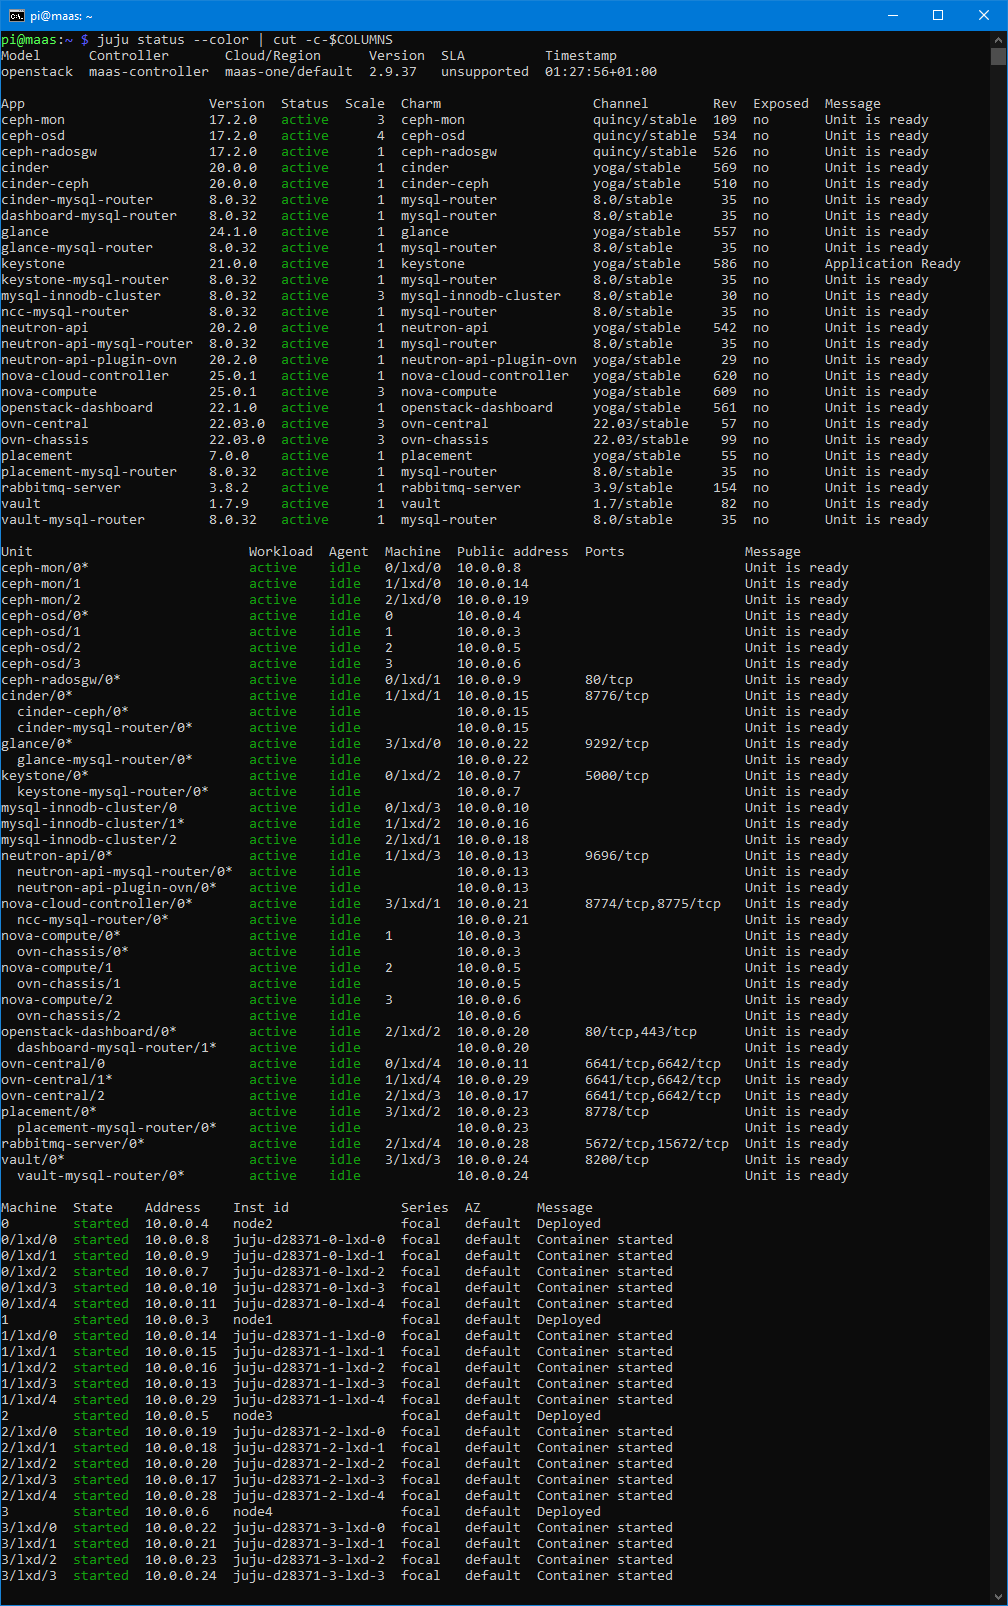
\includegraphics[width=1\linewidth]{tesi/files/immagini/openstack/finish.png}
%     \vspace*{-8mm}
%     \caption{Status finale del cloud OpenStack post deployment con i charm.}
%     \label{fig:juju_status_finish}
% \end{figure}

\begin{figure}%[H]
    \centering
    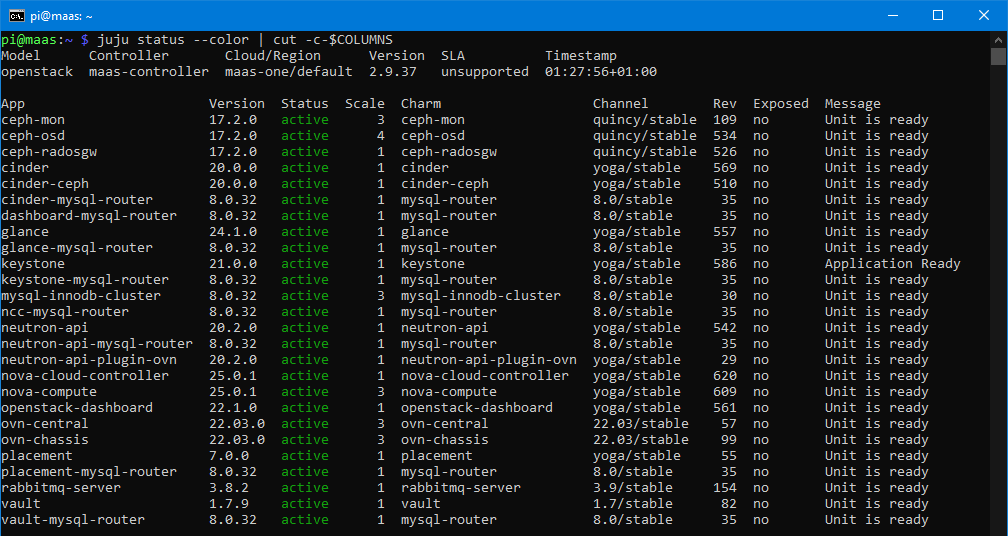
\includegraphics[width=1\linewidth]{tesi/files/immagini/openstack/finish(app).png}
    % \vspace*{-8mm}
    \caption{Status finale del cloud OpenStack post deployment con i charm: elenco delle App (i message sono tagliati per motivi di spazio).}
    \label{fig:juju_status_finish_app}
\end{figure}

\begin{figure}%[H]
    \centering
    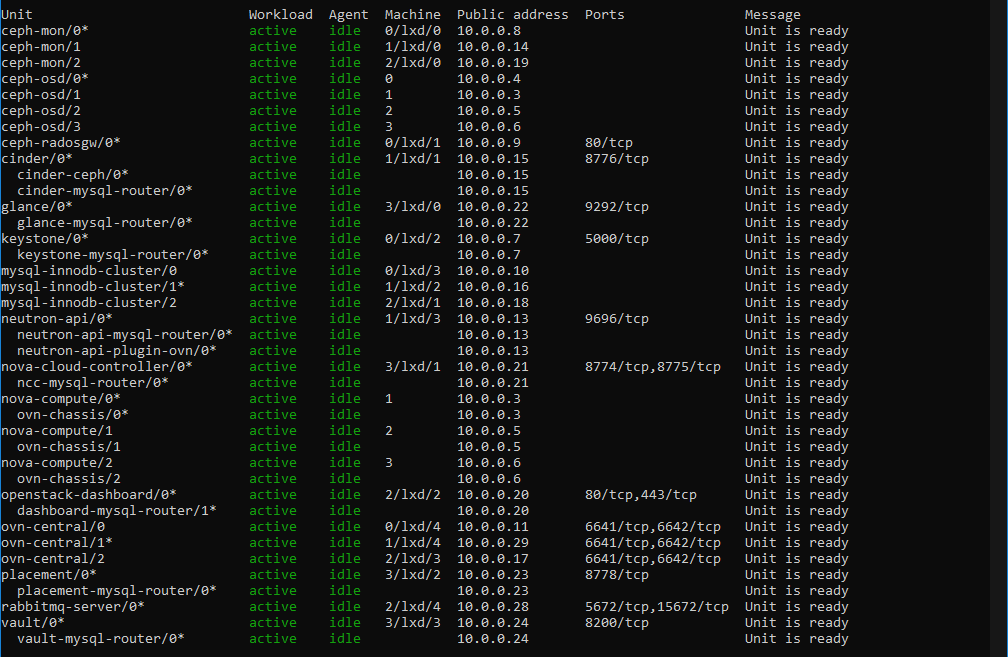
\includegraphics[width=1\linewidth]{tesi/files/immagini/openstack/finish(unit).png}
    % \vspace*{-8mm}
    \caption{Status finale del cloud OpenStack post deployment con i charm: elenco delle Unit (i message sono tagliati per motivi di spazio).}
    \label{fig:juju_status_finish_unit}
\end{figure}

\begin{figure}%[ht]
    \centering
    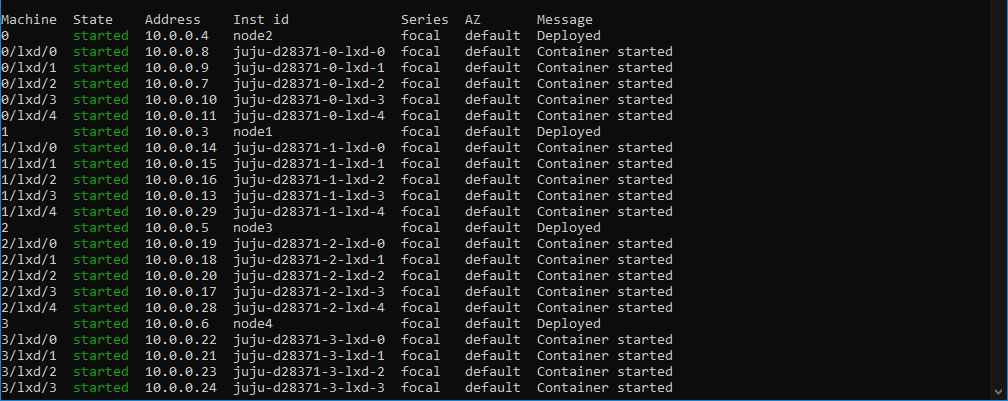
\includegraphics[width=1\linewidth]{tesi/files/immagini/openstack/finish(machine).png}
    % \vspace*{-8mm}
    \caption{Status finale del cloud OpenStack post deployment con i charm elenco delle Machine.}
    \label{fig:juju_status_finish_machine}
\end{figure}



\subsection{Accesso alla dashboard Horizon.}\label{subsec:openstack_dashboard}
Ora è finalmente possibile utilizzare il cloud OpenStack.
% 
Come prima cosa, bisogna ricavare i dati per poter accedere alla dashboard del cloud.
% 
Per ricavare l'indirizzo IP della web app è possibile sia cercarlo manualmente sotto la unit \code{openstack-dashboard/0*} nell'output del comando \code{juju status} (come mostrato in \cref{fig:juju_status_finish_unit}) sia estrapolarlo utilizzando la combinazione di comandi mostrati nel \cref{lst:openstack_install_ip_dashboard}.
% \begin{minipage}{0.96\linewidth} 
\begin{lstlisting}[
    language=mybash, 
   caption={Comandi per estrapolare l'IP della dashboard Horizon. },
    label={lst:openstack_install_ip_dashboard},
]
juju status --format=yaml openstack-dashboard | grep public-address | awk '{print $2}' | head -1
\end{lstlisting}
% \end{minipage}
In questo progetto di testi, l'indirizzo IP che è stato riservato in maniera automatica al charm openstack-dashboard è \code{10.0.0.20}.
 
% \bigskip\noindent
\vspace{1cm}\noindent
Dopodiché, è necessario conoscere le credenziali dell'amministratore di sistema.
% 
La password può essere richiesta a Keystone come mostrato nel seguente listato \cref{lst:openstack_install_credenziali}.
% \begin{minipage}{0.96\linewidth} 
\begin{lstlisting}[
    language=mybash, 
   caption={Richiesta a Keystone della password d'amministratore.},
    label={lst:openstack_install_credenziali},
]
juju run --unit keystone/leader leader-get admin_passwd
\end{lstlisting}
% \end{minipage}

% \begin{figure}[H]
%     \centering
%     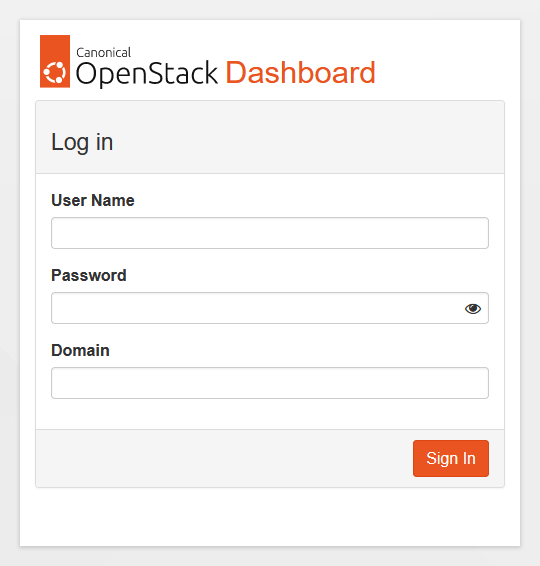
\includegraphics[width=0.7\linewidth]{tesi/files/immagini/openstack/login.png}
%     \caption{Schermata di login della dashboard di OpenStack.}
%     \label{fig:openstack_login}
% \end{figure}

\bigskip\noindent
L'URL della web app a cui collegarsi quindi sarà \code{http://<IP>/horizon/}\\
(o se si volesse usare il protocollo https \code{https://<IP>/horizon/}), in questo caso:
% 
\begin{itemize}
    \item[]URL: \textbf{http://10.0.0.20/horizon/}
\end{itemize}
% 
Una volta collegatosi da qualsiasi browser web
all'indirizzo, apparirà la schermata di log-in come mostrato in \cref{fig:openstack_login}.

\begin{figure}[H]
    \centering
    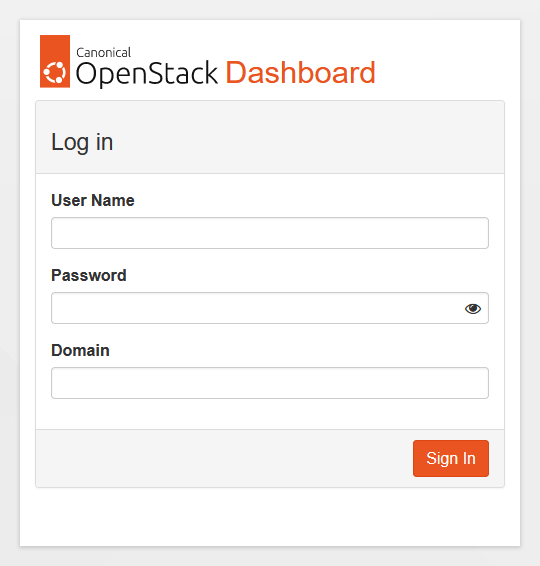
\includegraphics[width=0.5\linewidth]{tesi/files/immagini/openstack/login.png}
    \caption{Schermata di login della dashboard di OpenStack.}
    \label{fig:openstack_login}
\end{figure}

\bigskip
Le credenziali dell'amministratore da immettere sono:
% 
\begin{itemize}
    \item[]Username: \textbf{admin}
    
    \item[]Password: \textbf{ejco3C6Wgxj2je9B}
    
    \item[]Domain: \textbf{admin\_domain}
\end{itemize}

\bigskip\noindent
A log-in effettuato, apparirà la schermata iniziale, da cui poter utilizzare il cloud (\cref{fig:openstack_dashboard}).

\begin{figure}[H]
    \centering
    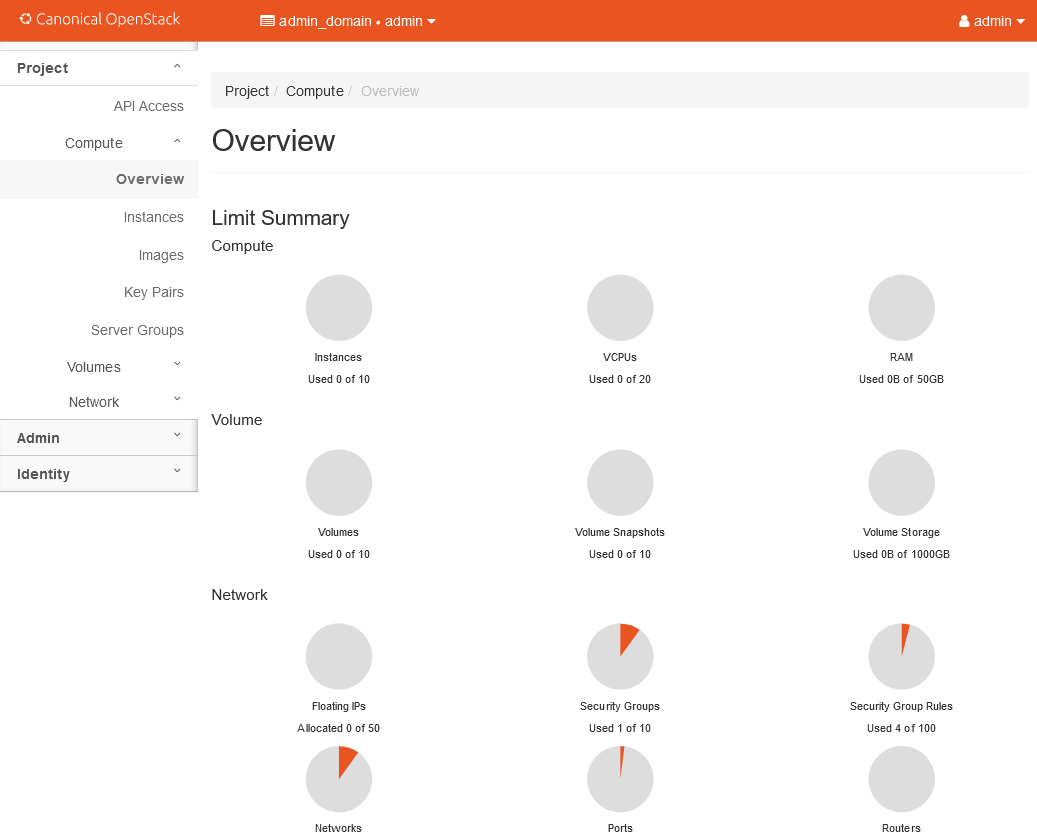
\includegraphics[width=0.95\linewidth]{tesi/files/immagini/openstack/dashboard.png}
    \caption{Schermata post log-in della dashboard di OpenStack con qualche risorsa in uso.}
    \label{fig:openstack_dashboard}
\end{figure}

\newpage

\section{Installazione in bundle}\label{sec:openstack_installazione_bundle}

Come accennato in precedenza all'interno del capitolo riguardante Juju, un bundle è un file yaml contenente la lista di tutti i charm che si vogliono installare con le relative configurazioni; è possibile inoltre definire delle variabili all'interno del file bundle che poi potranno essere utilizzate come parametri di configurazione di uno o più charm.

All'interno del \cref{lst:openstack_bundle_example} è riportato un esempio estratto dal bundle realizzato durante lo svolgimento di questo progetto, che mostra in che modo deve essere strutturata la configurazione di un charm (l'intero bundle è consultabile in \cref{app:openstack_bundle}).

\begin{lstlisting}[
    language=yaml, 
   caption={Esempio di configurazione di un charm all'interno del bundle.},
    label={lst:openstack_bundle_example},
]
variables:
    osd-devices: &osd-devices /dev/sdb /dev/sdc
    openstack-origin: &openstack-origin cloud:focal-yoga
    ceph-channel: &ceph-channel quincy/stable
applications:
    ceph-osd:
        charm: ch:ceph-osd
        channel: *ceph-channel
        num_units: 4
        options:
          osd-devices: *osd-devices
          source: *openstack-origin
        to:
        - '0'
        - '1'
        - '2'
        - '3'

\end{lstlisting}

Come si può notare dall'esempio sopra la variabili devono essere definite all'intenro della chiave \emph{variables} e devono avere il seguente formato:\newline
\verb|nome-variabile: &nome-variabile valore|.
Possono essere richiamate utilizzando la sintassi seguente: \verb|*nome-variabile|

Per quanto riguarda i charm, ciascuno di essi deve essere definito all'interno della chiave \emph{applications}. Come si può vedere dall'esempio nel \cref{lst:openstack_bundle_example}, il charm (in questo caso \emph{ceph-osd}) ha diversi parametri di configurazione: alcuni sono comuni a tutti i charm mentre altri sono specifici per il charm che si sta configurando. I parametri in comune tra tutti i charm sono i seguenti:
\begin{itemize}
    \item \textbf{charm}: indica il charm da installare (il prefisso \emph{ch:} indica che deve essere scaricato da Charmhub)
    \item \textbf{channel}: indica la versione del charm
    \item \textbf{num\_units}: indica il numero di istanze che devono essere eseguite
    \item \textbf{options}: al suo interno devono essere specificate tutti le configurazioni specifiche del charm
    \item \textbf{to}: indica le macchine sulle quali deve essere installato il charm; se viene inserito solamente il numero della macchina il charm verrà installato direttamente sul sistema operativo host mentre se viene specificato nel formato \verb|lxd:<id_macchina>| verrà istanziato un container sulla macchine selezionata all'interno del quale verrà installato il charm
\end{itemize}

\paragraph{Generazione del bundle.} La generazione del bundle è un'operazione abbastanza complessa che può richiedere molto tempo e durante la quale è facile fare piccoli errori che causerebbero il malfunzionamento di tutto il sistema. Per questo motivo esiste una funzionalità di Juju che permette di generare un bundle partendo da un deployment già esistente. Questa operazione può essere eseguita semplicemente lanciando il comando \verb|juju export-bundle|.

Durante lo svolgimento di questo progetto è stato tentato questo approccio però sono stati riscontrati diversi problemi a causa dei quali non è stato possibile installare OpenStack utilizzando solamente il bundle generato da Juju. La soluzione adottata è stata quella di fare un'unione manuale tra il bundle generato e quello di esempio messo a disposizione da OpenStack \cite{openstack_example_bundle}.

\paragraph{Deploy del bundle} Una volta generato il bundle è possibile eseguire il deploy semplicemente lanciando il comando \verb|juju deploy ./bundle.yaml|.
È importante che il nome del file bundle sia inserito come percorso anche se si trova nella cartella corrente perché in caso contrario Juju lo tratterebbe come se fosse il nome di un charm e ovviamente l'installazione fallirebbe.

Una volta conclusa l'installazione dei charm sarà comunque necessario eseguire la configurazione iniziale di \emph{Vault} manualmente seguendo la procedura utilizzata durante l'installazione manuale di OpenStack e descritta nella \cref{subpar:vault_configuration}.
\newpage

\section{Configurazione iniziale}\label{sec:openstack_configurazioni_iniziali}
In questo capitolo verrà trattata la configurazione iniziale di un cloud OpenStack. Tutta la configurazione verrà fatta seguendo la guida di installazione \cite{openstack_configure} e di conseguenza utilizzando il tool a linea di comando, però è possibile anche eseguire tutte le operazione descritte in questo capitolo tramite l'interfaccia web. È possibile ottenere le credenziali dell'utente \verb|admin| eseguendo il comando \code{juju run -{}-unit keystone/leader leader-get admin\_passwd} dall'host su cui è stato precedentemente installato e configurato il client Juju.
% 
Per maggiori dettagli su come ottenere l'accesso, consultare la \cref{subsec:openstack_dashboard}.

Per comprendere meglio le configurazioni utilizzate in questa sezione, sia lato amministratore che utente, si consiglia di visionare la \cref{sec:openstack_usage} dove viene fornita una spiegazione dei concetti di base che permette di comprendere meglio quali sono le funzionalità di OpenStack e in che modo possono essere sfruttate.


\paragraph{Installazione del client e accesso al cloud.}
Per eseguire la configurazione tramite linea di comando è necessario installare il client OpenStack tramite il package manager (\texttt{snap} in questo caso) e clonare il repository openstack-bundles\footnote{OpenStack Bundle repository: \url{https://github.com/openstack-charmers/openstack-bundles}, ultimo accesso 28 Febbraio 2023}. 
% 
Per fare questo si devono eseguire i comando mostrati nel \cref{lst:openstack_config_install_client}

\begin{lstlisting}[
    language=mybash, 
    caption={Installazione del client openstack e clonazione del repo.},
    label={lst:openstack_config_install_client},
]
sudo snap install openstackclients
git clone https://github.com/openstack-charmers/openstack-bundles %*$\sim$*)/openstack-bundles
\end{lstlisting}

\noindent
In questo modo il repo verrà clonato nella home dell'utente e successivamente sarà sufficiente eseguire il comando nel \cref{lst:openstack_config_set_env} per impostare le variabili d'ambiente in modo da avere accesso al cloud con privilegi di amministrazione.

\begin{lstlisting}[
    language=mybash, 
    caption={Configurazione dell'accesso al cloud.},
    label={lst:openstack_config_set_env},
]
source %*$\sim$*)/openstack-bundles/stable/openstack-base/openrc
\end{lstlisting}


\subsection{Configurazioni da parte dell'amministratore}
\paragraph{Immagini e Flavor.}
Il primo passo è quello di creare la prima immagine e il primo flavor. Eseguendo i comandi nel \cref{lst:openstack_config_download_image} viene create la cartella \verb|cloud-images| nella home e al suo interno viene scaricata un'immagine recente di Ubuntu Jammy direttamente dall'archivio delle cloud images di Canonical; 
in questo modo sarà poi possibile ricaricare l'immagine sul nuovo cloud.

\begin{lstlisting}[
    language=mybash, 
    caption={Download dell'immagine di Ubuntu Jammy server.},
    label={lst:openstack_config_download_image},
]
mkdir %*$\sim$*)/cloud-images
curl http://cloud-images.ubuntu.com/jammy/current/jammy-server-cloudimg-amd64.img --output %*$\sim$*)/cloud-images/jammy-amd64.img
\end{lstlisting}

\noindent
Una volta terminato il download è possibile creare una nuova immagine partendo da quella scaricata eseguendo il comando nel \cref{lst:openstack_config_create_image}.

\begin{lstlisting}[
    language=mybash, 
    caption={Creazione di un'immagine partendo dal file scaricato.},
    label={lst:openstack_config_create_image},
]
openstack image create --public --container-format bare --disk-format qcow2 --file %*$\sim$*)/cloud-images/jammy-amd64.img jammy-amd64
\end{lstlisting}

\begin{itemize}
    \item \verb|--public|: indica che l'immagine è pubblica, ovvero è visibile a tutti gli utenti del cloud
    \item \verb|--container-format|: indica il formato del container dell'immagine, ovvero per quale tecnologia di virtualizzazione o containerizzazione è stata create l'immagine (per esempio \verb|bare| per macchine virtuali, \verb|docker| per container docker, ecc.)
    \item \verb|--disk-format|: indica il formato dell'immagine
    \item \verb|--file|: permette di specificare un file locale dal quale leggere l'immagine
    \item Come ultimo argomento deve essere inserito il nome dell'immagine
\end{itemize}


\medskip\noindent
Successivamente è possibile creare un flavor eseguendo il comando nel \cref{lst:openstack_config_create_flavor} (per maggiori informazioni sui flavor si veda la \cref{sec:flavor}).
%con i seguenti parametri:

\begin{lstlisting}[
    language=mybash, 
    caption={Creazione di un flavor.},
    label={lst:openstack_config_create_flavor},
]
openstack flavor create --ram 2048 --disk 20 --ephemeral 20 m1.small
\end{lstlisting}
\begin{itemize}
    \item \verb|--vcpus|: numero di CPU virtuali (di default impostato a 1)
    \item \verb|--ram|: quantità di memoria RAM espressa in MB
    \item \verb|--ephemeral|: dimensione dello storage storage temporaneo espresso in GB (utilizzato nel caso in cui non venga creato un volume per l'istanza)
    \item Come ultimo argomento deve essere inserito il nome del flavor
\end{itemize}


\paragraph{Rete pubblica.}
Dopo aver creato la prima immagine e il primo flavor è necessario configurare la rete pubblica, ovvero la rete che permette alle istanze di tutto il cloud di comunicare con l'esterno. Per fare questo è necessario prima di tutto creare la rete eseguendo i comandi nel \cref{lst:openstack_config_create_public_network}.

\begin{lstlisting}[
    language=mybash, 
    caption={Creazione di una rete pubblica.},
    label={lst:openstack_config_create_public_network},
]
openstack network create --external --share --provider-network-type flat --provider-physical-network physnet1 ext_net
\end{lstlisting}

\begin{itemize}
    \item \verb|--external|: indica che è una rete pubblica
    \item \verb|--share|: indica che la rete è condivisa tra tutti gli utenti del cloud
    \item \verb|---provider-network-type|: permette di specificare il meccanismo fisico con il quale la rete virtuale è implementata; in questo caso \verb|flat| significa che utilizza una scheda di rete fisica configurata come bridge
    \item \verb|--provider-physical-network|: nome della rete fisica sulla quale la rete virtuale si appoggia
    \item Come ultimo argomento deve essere inserito il nome della nuova rete.
\end{itemize}

\medskip\noindent
Dopo aver creato la rete è possibile creare anche la subnet utilizzando il comando mostrato nel \cref{lst:openstack_config_create_public_subnet}.
% con i seguenti parametri:

\begin{lstlisting}[
    language=mybash, 
    caption={Creazione di una subnet pubblica.},
    label={lst:openstack_config_create_public_subnet},
]
openstack subnet create --network ext_net --no-dhcp --gateway 10.0.0.1 --subnet-range 10.0.0.0/24 --allocation-pool start=10.0.0.40,end=10.0.0.99 ext_subnet
\end{lstlisting}
\begin{itemize}
    \item \verb|--network|: nome della rete dentro la quale creare la subnet
    \item \verb|--no-dhcp|: se specificato il DHCP viene disabilitato per la nuova subnet
    \item \verb|--gateway|: indirizzo IP del gateway
    \item \verb|--subnet-range|: permette di specificare il range di indirizzi IP appartenenti alla subnet (in formato CIDR)
    \item \verb|--allocation-pool|: permette di specificare il pool di indirizzi IP assegnabili dinamicamente (nel formato \verb|start_ip,end_ip|). Questo pool può risiedere anche nella sottorete di MAAS. Quindi bisogna riservare questi indirizzi in modo tale che non li utilizzi. Per farlo, bisogna connettersi alla dashboard di MAAS, preme in alto su \emph{Subnets} e selezionare la VLAN. Poi, bisogna premere sul pulsante \emph{Reserve Range} (NON \emph{dynamic}) ed inserire i due indirizzi IP del pool.
    % matteo si è scordato di spiegare l'aggiunta degli ip  riservati su maas...
 \item Come di consueto l'ultimo argomento deve essere il nome della nuova subnet.
\end{itemize}


\paragraph{Dominio, Progetto e Utente.}
A questo punto può considerarsi conclusa la configurazione delle risorse condivise ed è possibile iniziare a configurare le risorse per gli utilizzatori del cloud, ovvero domini, progetti e utenti.

Il primo passo è quello di creare un dominio, perché senza quest'ultimo non è possibile aggiungere progetti o utenti al di fuori del dominio di amministrazione. Successivamente, si possono creare il progetto, specificando il domain in cui inserirlo, e l'utente, specificando il progetto e il dominio di cui appartiene. Questi tre comandi sono esplicitati nel \cref{lst:openstack_config_create_domain_project_user}.

\begin{lstlisting}[
    language=mybash, 
    caption={Creazione di dominio, progetto e utente.},
    label={lst:openstack_config_create_domain_project_user},
]
openstack domain create domain1
openstack project create --domain domain1 project1
openstack user create --domain domain1 --project project1 --password-prompt user1
\end{lstlisting}
\begin{itemize}
    \item Con \verb|--password-prompt| la password verrà richiesta a terminale una volta eseguito il comando.
\end{itemize}

\medskip\noindent
Dopo aver creato l'utente è necessario assegnargli un ruolo in base ai permessi che gli si vogliono consentire. In questo caso verrà assegnato il ruolo \verb|Member| al nuovo utente utilizzando il comando mostrato nel \cref{lst:openstack_config_set_user_role}; in questo modo che potrà effettuare tutte quelle operazioni che non richiedono permessi di amministrazione.

\begin{lstlisting}[
    language=mybash, 
    caption={Assegnazione del ruolo al nuovo utente.},
    label={lst:openstack_config_set_user_role},
]
openstack role add --user 8b16e5335976418e99bf0b798e83e413 --project project1 Member
\end{lstlisting}

\bigskip\noindent
A questo punto è possibile iniziare ad utilizzare il cloud con il nuovo utente appena creato. 
% 
% Per fare un primo test e verificare che tutto funzioni correttamente si può procedere nel seguente ordine:
% \begin{enumerate}
%     \item Creazione di una rete privata e di una subnet
%     \item Creazione di un router per collegare la rete pubblica con quella privata
%     \item Creazione o inserimento di una coppia di chiavi pubbliche-private
%     \item Creazione di un'istanza
%     \item Assegnazione di un floating IP alla nuova istanza
% \end{enumerate}

% \medskip\noindent
% Tutte le istruzioni per eseguire le operazioni sopra citate si trovano nel \cref{sec:openstack_usage} insieme ad una spiegazione dei concetti di base che permettono di comprendere meglio quali sono le funzionalità di OpenStack e in che modo possono essere sfruttate.



\subsection{Configurazioni da parte dell'utente}
\paragraph{Setup ambiente utente.}
Prima di iniziare ad utilizzare il nuovo utente, è necessario configurare le variabili d'ambiente del terminale per poter eseguire i comandi \texttt{openstack} con questi privilegi.
% 
Come prima cosa, bisogna prelevare l'URL di \emph{Keystone} per l'autenticazione; 
% 
è possibile ricavarlo tramite il comando \code{juju status} o più semplicemente, si può ricavare dall'ambiente amministratore utilizzato in precedenza dalla variabile \texttt{OS\_AUTH\_URL}.
% 
Quindi basterà eseguire sul terminale \code{echo \$OS\_AUTH\_URL} per avere in output l'URL.

A questo punto, si può creare un file con le configurazioni d'esempio mostrate nel \cref{lst:openstack_ambiente_utente}.
% 
In questo caso il file verrà chiamato \emph{project1-rc} (senza estensione).

\begin{lstlisting}[
    language=mybash, 
    caption={File per l'ambiente utente \emph{user1}.},
    label={lst:openstack_ambiente_utente},
]
export OS_AUTH_URL=https://10.0.0.7:5000/v3
export OS_USER_DOMAIN_NAME=domain1
export OS_USERNAME=user1
export OS_PROJECT_DOMAIN_NAME=domain1
export OS_PROJECT_NAME=project1
export OS_PASSWORD=ubuntu
\end{lstlisting}
\begin{itemize}
    \item I valori delle variabili sono i medesimi creati per l'utente nel \cref{lst:openstack_config_create_domain_project_user}.
    \item Per la password, si è ipotizzato che è stata inserita \emph{ubuntu}.
\end{itemize}

\noindent
Una volta salvato il file, è possibile eseguire il comando \code{source project1-rc} per impostare le variabili d'ambiente per avere eccesso al cloud con l'utente scelto.
% 
Ora è possibile utilizzare il cloud con l'utente attraverso la riga di comando.



\paragraph{Rete Privata.}
Come prima cosa, verrà configurata la rete privata che verrà poi utilizzata dalle varie macchine virtuali.
% 
Si eseguano i comandi nel \cref{lst:openstack_config_create_private_network} per poterla creare.

\begin{lstlisting}[
    language=mybash, 
    caption={Creazione di una rete privata con la relativa subnet.},
    label={lst:openstack_config_create_private_network},
]
openstack network create --internal user1_net

openstack subnet create --network user1_net --dns-nameserver 10.0.0.2 --subnet-range 192.168.0/24 --allocation-pool start=192.168.0.10,end=192.168.0.199 user1_subnet
\end{lstlisting}

\begin{itemize}
    \item \verb|--internal|: indica che si tratta di una rete privata
    
    \item \verb|--dns-nameserver|: indica l'indirizzo del DNS utilizzato
    
    \item Come ultimo argomento dei due comandi deve essere inserito il nome della nuova rete e della nuova subnet
\end{itemize}

\noindent
Creata la rete, è necessario creare un router virtuale per poter collegare la rete pubblica con la rete appena creata.
% 
I comandi mostrati in  mostrano la creazione del router.
\begin{lstlisting}[
    language=mybash, 
    caption={Creazione di una router virtuale.},
    label={lst:openstack_config_create_router},
]
openstack router create user1_router
openstack router add subnet user1_router user1_subnet
openstack router set user1_router --external-gateway ext_net
\end{lstlisting}
\begin{itemize}
    \item \verb|--external-gateway|: indica il nome della rete esterna creata nel \cref{lst:openstack_config_create_public_network}
    
    \item Come ultimo argomento del primo comando deve essere inserito il nome del nuovo router
\end{itemize}



\paragraph{Import chiavi SSH e Security Group.}
Per poter accedere alle istanze delle macchine virtuali, è necessario importare una coppia di chiavi SSH.
% 
Nel \cref{lst:openstack_config_import_key} è mostrato come viene importata la chiave pubblica SSH all'interno di OpenStack.

\begin{lstlisting}[
    language=mybash, 
    caption={Importazione delle chiavi SSH.},
    label={lst:openstack_config_import_key},
]
openstack keypair create --public-key %*$\sim$*)/.ssh/id_rsa.pub user1
\end{lstlisting}
\begin{itemize}
    \item \verb|--public-key|: indica il path della chiave pubblica
        
    \item Come ultimo argomento deve essere inserito il nome da associare alla \emph{Key Pairs}
\end{itemize}

\noindent
Per consentire il passaggio del traffico SSH nelle future macchine virtuali, è necessario creare un \emph{Security Group} come mostrato nel \cref{lst:openstack_config_create_security_group}, avente le varie regole per consentire il traffico su determinati protocolli e porte.
\begin{lstlisting}[
    language=mybash, 
    caption={Creazione del Security Group per il traffico SSH.},
    label={lst:openstack_config_create_security_group},
]
openstack security group create --description 'Allow SSH' Allow_SSH
openstack security group rule create --proto tcp --dst-port 22 Allow_SSH
\end{lstlisting}
\begin{itemize}
    \item \verb|--description|: è la descrizione del gruppo di regole da creare
        
    \item \verb|--proto|: indica il protocollo della regola
        
    \item \verb|--dst-port|: indica la porta della regola
        
    \item Come ultimo argomento dei due comandi deve essere inserito il nome da associare al \emph{Security Group} e alla relativa regola
\end{itemize}



\paragraph{Creazione di una istanza.}
Finalmente è possibile creare una macchina virtuale.
% 
Per farlo è sufficiente eseguire il comando mostrato nel \cref{lst:openstack_config_create_istance}
\begin{lstlisting}[
    language=mybash, 
    caption={Creazione di una istanza della macchina virtuale.},
    label={lst:openstack_config_create_istance},
]
openstack server create --image jammy-amd64 --flavor m1.small --key-name user1 --network user1_net --security-group Allow_SSH jammy-1
\end{lstlisting}
\begin{itemize}
    \item \verb|--image|: viene indicata l'immagine da utilizzare
    
    \item \verb|--flavor|: viene indicato il flavor da utilizzare

    \item \verb|--key-name|: viene indicato il nome della key pair da utilizzare
        
    \item \verb|--network|: indica il nome della rete privata su cui la macchina virtuale si collegherà  
        
    \item \verb|--security-group|: indica il gruppo di regole per consentire il traffico dati
        
    \item Come ultimo argomento deve essere inserito il nome da associare alla istanza della macchina virtuale
\end{itemize}

\noindent
Al termine ella creazione della macchina virtuale, è possibile associargli un indirizzo pubblico per poter poi collegarsi in SSH.
% 
Anche questa volta, nel \cref{lst:openstack_config_create_floating_ip} verrà mostrato come poter eseguire questa fase.
\begin{lstlisting}[
    language=mybash, 
    caption={Creazione e associazione di un floating ip alla vm.},
    label={lst:openstack_config_create_floating_ip},
]
FLOATING_IP=$(openstack floating ip create -f value -c floating_ip_address ext_net)
openstack server add floating ip jammy-1 $FLOATING_IP
\end{lstlisting}

\noindent
Una volta eseguito, si avrà l'indirizzo IP pubblico all'interno della variabile \texttt{FLOATING\_IP}, e pertanto è possibile utilizzarlo per connettersi in SSH alla macchina virtuale.

\bigskip
\noindent
Si conclude qui l'installazione e l'uso base del cloud OpenStack.
% 
Nel \cref{sec:openstack_usage} è possibile approfondire gli aspetti trattati in questa sezione, mentre nella \cref{sec:terraform} è stato utilizzato lo strumento Terraform per poter creare le varie risorse di OpenStack tramite del codice di configurazione.

\newpage

\chapter{Utilizzo di OpenStack}\label{sec:openstack_usage}

All'interno di questo capitolo verranno spiegati tutti i concetti base che servono per un primo utilizzo di OpenStack. Verranno anche date le istruzioni per eseguire le operazioni principali, come ad esempio creare una rete o una macchina virtuale, in modo che anche chi non ha mai utilizzato questa piattaforma possa orientarsi e farsi un'idea generale sulle funzionalità che offre.

\section{Identity}

\subsection{Domains}

Un dominio di OpenStack è un contenitore ad alto livello per progetti, gruppi e utenti. Ciascun dominio definito all'interno di un cloud OpenStack è completamente indipendente dagli altri; questo permette di avere entità (per esempio utenti, gruppi o progetti) con gli stessi nomi definiti in domini diversi. Inoltre gli utenti di domini diversi possono essere rappresentati da diversi backend di autenticazione e avere attributi diversi ma devono obbligatoriamente essere mappati sugli stessi set di ruoli e privilegi che sono stati utilizzati per definire le policy di sicurezza in modo da poter avere accesso ai servizi del cloud.

Per creare un dominio è necessario accedere con un utente amministratore. Una volta eseguito il login si deve aprire il menu a tendina denominato \textit{Identity} e selezionare la voce \textit{Domains}. A questo punto verrà visualizzata la pagina con tutti i domini presenti all'interno del cloud e per crearne uno nuovo sarà sufficiente cliccare sul pulsante \textit{Create Domain} e inserire i dati richiesti. Se si vogliono aggiungere entità al dominio appena creato (per esempio utenti, progetti, ecc.) sarà necessario cliccare sul pulsante \textit{Set Domain Context} accanto al nome del dominio; in questo modo il context della sessione verrà cambiato in modo da attivare il dominio selezionato e poter modificare le sua entità.

\subsection{Groups}

I gruppi di OpenStack sono dei contenitori ai quali appartengono degli utenti. Possono essere utilizzati per garantire l'accesso a progetti o semplicemente per raggruppare gli utenti.

Per creare un gruppo è necessario accedere all'interfaccia con un utente amministratore o con privilegi di amministrazione all'interno del dominio. Una volta eseguito l'accesso si deve aprire il menu a tendina \textit{Identity} e selezionare la voce \textit{Groups}. Cliccando sul pulsante \textit{Create Group} verrà visualizzato un form tramite il quale sarà possibile creare il nuovo gruppo.

\subsection{Roles}

I ruoli sono delle entità associate agli utenti e, dato che OpenStack usa un approccio RBAS (Role-Based Access Control), servono per determinare quali azioni ciascun utente può compiere. 

\subsection{Projects}

Un progetto è un contenitore di entità (utenti, istanze, ecc.) che a sua volta fa parte di un dominio. A differenza di un dominio il progetto possiede alcune entità univoche e altre che possono essere in comune con altri progetti; per esempio un'istanza può far parte solamente di un progetto, mentre un utente può far parte di più progetti.

Per creare un progetto è necessario eseguire l'accesso all'interfaccia con un utente amministratore o con privilegi di amministrazione all'interno del dominio. Una volta eseguito l'accesso si deve aprire il menu a tendina \textit{Identity} e selezionare la voce \textit{Projects}. Cliccando poi sul pulsante \textit{Create Project} verrà aperto un form composto da tre schede:
\begin{itemize}
    \item \textbf{Project Information}: permette di specificare le informazioni generiche del progetto (nome, descrizione, ecc.)
    \item \textbf{Project Members}: permette di selezionare gli utenti che hanno accesso al progetto
    \item \textbf{Project Groups}: permette di selezionare i gruppi che fanno parte del progetto
\end{itemize}

\noindent
Se si utilizza Horizon (l'interfaccia Web di OpenStack) è possibile accedere solamente ad un progetto per volta, ovvero visualizzare le entità del progetto selezionato. Per cambiare la selezione del progetto è necessario cliccare sul nome del progetto attualmente selezionato nella barra di navigazione in cima alla pagine (come mostrato in \cref{fig:openstack_project_selection}) e successivamente selezionare dal menu a tendina il progetto che si vuole utilizzare.

\begin{figure}[H]
    \center
    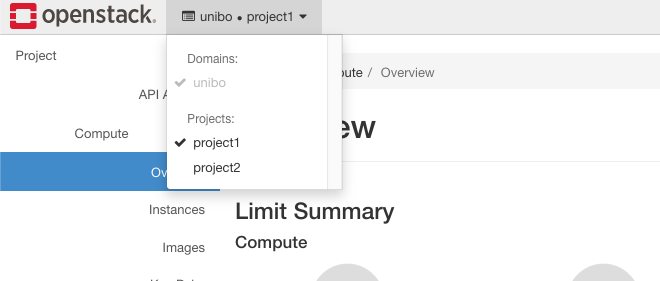
\includegraphics[width=0.9\linewidth]{tesi/files/immagini/openstack_usage/openstack_project_switch.png}
    \caption{Selezione del progetto tramite l'interfaccia Web.}
    \label{fig:openstack_project_selection}
\end{figure}

\subsection{Users}

Gli user, come ci su può aspettare, sono gli utenti che utilizzano il cloud OpenStack. Ciascun utente può essere membro di uno o più progetti, di uno o più gruppi e può avere uno o più ruoli. È possibile autenticare gli utenti in modi differenti utilizzando provider di autenticazione esterni (per esempio LDAP, SSO, ecc.); nel caso di questo progetto è stato utilizzato il provider di default di OpenStack.

Per creare un utente è necessario eseguire l'accesso all'interfaccia con un utente amministratore o con privilegi di amministrazione all'interno del dominio. Una volta eseguito l'accesso si deve aprire il menu a tendina \textit{Identity} e selezionare la voce \textit{Users}. In questo modo verrà aperta la pagine contenente tutti gli utenti del dominio che si sta visualizzando e, cliccando sul pulsante \textit{Crete User} in alto a destra, sarà possibile crearne uno nuovo. È possibile inserire numerose informazioni riguardanti ciascun utente ma quelle fondamentali sono Username, Password e Primary Project; se non viene scelto nessun progetto verrà negato l'accesso al nuovo utente nonostante sia abilitato.

\section{Network}

\subsection{Networks e Subnets}

Una network in OpenStack è una rete virtuale che sta alla base della comunicazione tra macchine virtuali, container o altri dispositivi virtuali che comunicano tramite rete.
% 
Ciascuna network può contenere al suo interno una o più subnet che hanno la stessa funzionalità delle VLAN in una rete fisica: 
% 
servono per suddividere logicamente la rete in più sezioni separate, ciascuna delle quali possiede un proprio range di indirizzi IP ed è indipendente dalle altre.

Per creare una rete è necessario aprire il menu a tendina \textit{Project} > \textit{Network} e selezionare la voce \textit{Networks}; questo aprirà la pagina dove vengono visualizzate tutte le reti. A questo punto, cliccando sul pulsante \textit{Create Network}, verrà visualizzato il form per creare la nuova rete. Spuntato la casella \textit{Enable Admin State} la rete verrà automaticamente abilitata dopo la creazione e, spuntando \textit{Create Subnet}, viene data anche la possibilità di creare direttamente una subnet. Tramite il parametro \textit{MTU} è possibile anche configurare la dimensione massima che possono avere i pacchetti che vengono inviati sulla rete.

Con un utente con privilegi di amministrazione è possibile anche creare una rete pubblica, ovvero una rete che possiede una subnet con indirizzi IP pubblici a cui tutti gli utenti possono collegarsi, in modo che gli host della rete possano essere raggiunti direttamente dall'esterno.

Per creare una subnet invece è necessario andare alla pagine dove vengono visualizzate tutte le reti e cliccare sul nome di quella che si vuole utilizzare; questo aprirà la pagina di dettaglio della rete. Una volte fatto questo si deve passare alla scheda denominata \textit{Subnets} e cliccare sul pulsante \textit{Subnets}; a questo punto verrà visualizzato un form suddiviso in due schede dove andranno inserite tutte le informazioni riguardanti la nuova subnet che si vuole creare. I campi richiesti sono i seguenti:
\begin{itemize}
    \item \textbf{Subnet Name}: nome della subnet (arbitrario)
    \item \textbf{Network Address}: spazio degli indirizzi IP (in formato CIDR) che appartengono alla subnet (per esempio \texttt{10.0.0.0/24})
    \item \textbf{IP Version}: versione del protocollo IP
    \item \textbf{Gateway IP}: indirizzo IP del gateway; se non si desidera aggiungere un gateway alla subnet è possibile spuntare la casella \texttt{Disable Gateway} per disabilitarlo
    \item \textbf{Enable DHCP}: se spuntato, il server DHCP viene abilitato per la nuova subnet
    \item \textbf{Allocation Polls}: permette di indicare i range di indirizzi IP che possono essere assegnati dinamicamente; si deve inserire un pool per ciascuna riga nel formato \texttt{start\_ip,end\_ip} (per es. \texttt{10.0.0.128,10.0.0.253})
    \item \textbf{DNS Name Servers}: permette di specificare i server DNS per la subnet (uno per riga)
    \item \textbf{Host Routes}: permette di specificare delle regole di routing statiche che verranno applicate agli host; ciascuna entry deve essere nel formato \texttt{destination\_cidr,nexthop} (per es. \texttt{192.168.1.0/24,10.0.0.1})
\end{itemize}

\subsection{Routers}

Un router virtuale OpenStack ha esattamente le stesse funzioni di un router fisico in una rete fisica: permette agli host della rete di raggiungere subnet diverse dalla propria. Il router supporta sia il routing statico sia diversi protocolli di routing dinamico, come ad esempio OSPF e BGP. Ciascun router può avere una o più interfacce virtuali che possono essere collegate a diverse subnet appartenenti alla stessa rete o a reti diverse. I router possono avere un numero indefinito di interffacce di rete virtuali e quindi possono essere collegati a tutte le subnet desiderate; inoltre, se una delle interfacce viene collegata ad una rete pubblica, permettono a ciascuno degli host presenti sulle subnet private di accedere a internet utilizzando la tecnica del NAT.

Per creare un router è necessario aprire il menu a tendine \textit{Project} > \textit{Network} e selezionare la voce \textit{Routers}; in questa pagina verranno mostrati tutti i router appartenenti al progetto corrente. Cliccando sul pulsante \textit{Create Router} verrà mostrato il form che permette di creare il nuovo router con i seguenti campi che, oltre a campi simili a quelli visti in precedenza, contiene il campo \emph{External Network} che permette di specificare una rete esterna a cui collegare il router. Questo campo non è obbligatorio ma se si desidera far accedere gli host delle subnet collegate al router a internet senza un indirizzo IP pubblico è necessario impostarlo.
% 
Dopo aver creato il router è possibile aggiungere le interfacce virtuali che lo collegano alle subnet; per fare questo si deve cliccare sul nome del router in modo da aprire la pagina con tutte le informazioni, aprire la scheda \textit{Iterfaces} e cliccare sul pulsante \textit{Add Interface}. A questo punto comparirà un form che permette di selezionare quale subnet collegare al router e opzionalmente l'indirizzo IP da assegnargli all'interno della subnet selezionata.

Nel caso in cui il router sia stato collegato ad una rete esterna, nella pagina di dettaglio con tutte le informazioni riguardanti il router è possibile visualizzare il suo indirizzo IP pubblico nella sezione \emph{External Gateway}. Questo permette di verificare se il router funziona semplicemente facendo un ping all'indirizzo mostrato.

\begin{figure}[ht]
   \center
   % 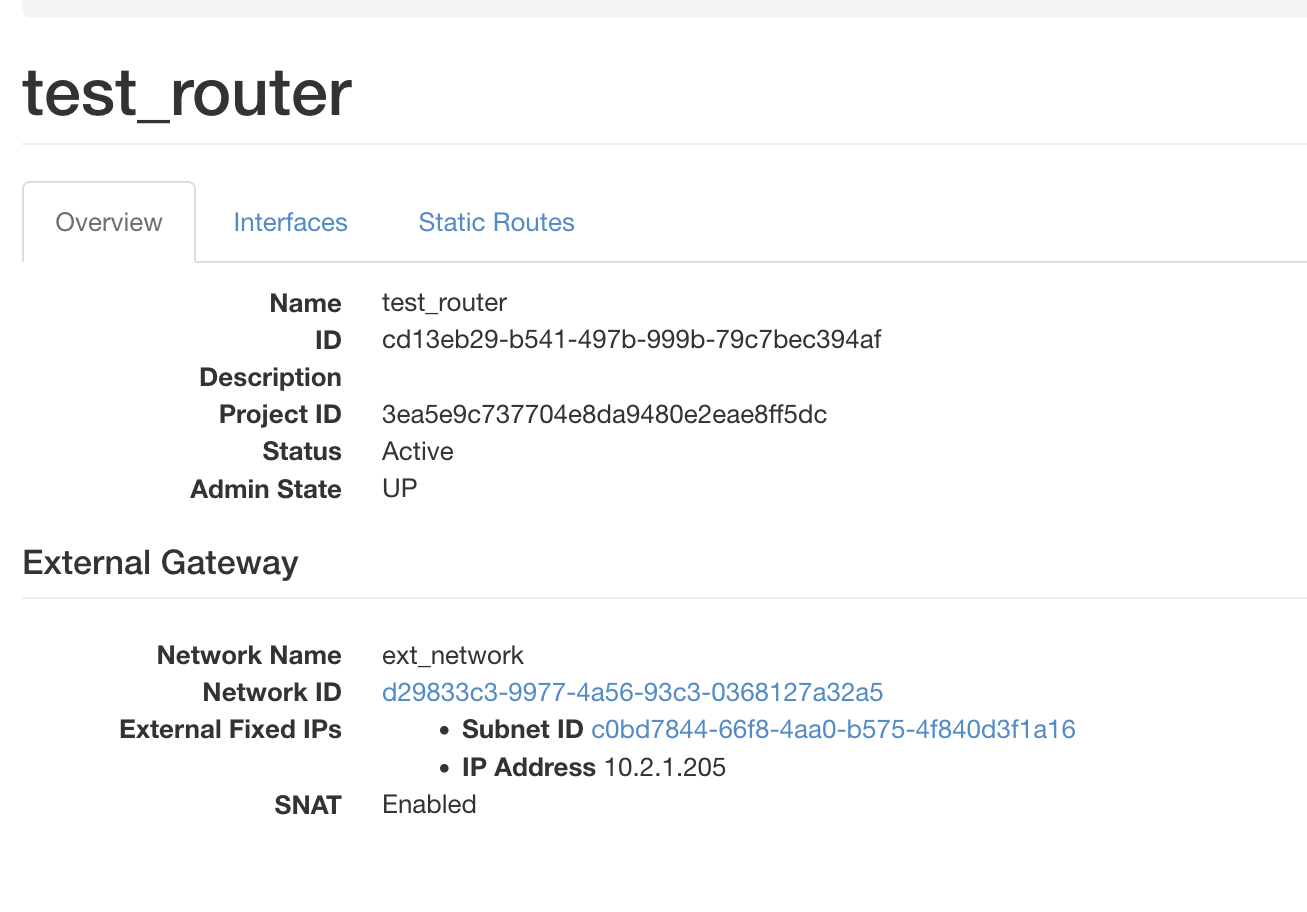
\includegraphics[scale=0.4]{tesi/files/immagini/openstack_usage/openstack_router_info.png}
   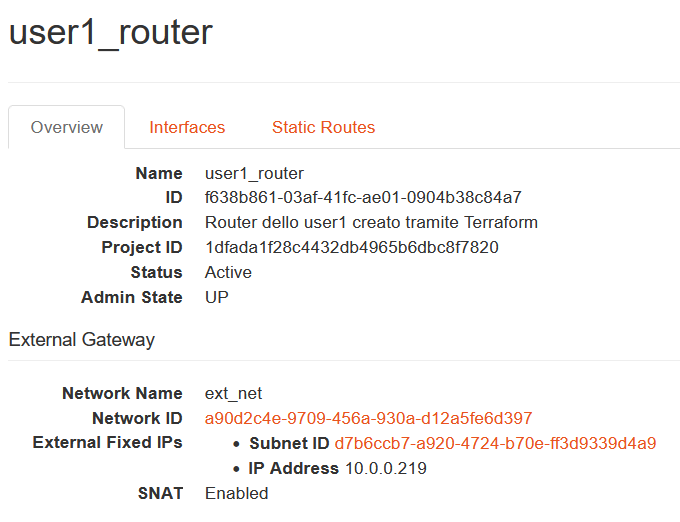
\includegraphics[width=0.9\linewidth]{tesi/files/immagini/openstack_usage/openstack_router_info_2.png}
   \caption{Pagina con le informazioni di un router.}
   \label{fig:openstack_router_info}
\end{figure}

\subsection{Security Groups}

I \textit{Security Groups} sono l'equivalente dei firewall virtuali che controllano il traffico in entrata e in uscita per ciascun host. Permettono di specificare regole secondo diversi criteri come ad esempio gli indirizzi IP della sorgente e del destinatario o le porte. Ciascun \textit{Security Group} può avere un numero indefinito di regole e può essere assegnato a più di un host; ogni host può avere a sua volta più di un \textit{Security Group}.

Per creare un \textit{Security Group} da interfaccia grafica è necessario aprire il menu a tendina \textit{Project} > \textit{Network} e cliccare sulla voce \textit{Security Groups}; in questo modo verrà aperta la pagina che mostra tutti i gruppi presenti all'interno del progetto corrente. Cliccando sul pulsante \textit{Create Security Group} in alto a destra verrà aperto un form che permetterà di specificare nome e descrizione del nuovo gruppo. Per modificare le regole del \textit{Security Group} appena creato si deve cliccare il pulsante \textit{Manage Rules} sulla stessa riga del nome; a questo punto verrà caricata una pagina con la lista delle regole già presenti; per crearne una nuova è necessario cliccare sul pulsante \textit{Add Rule} che farà comparire un form con i seguenti campi:
\begin{itemize}
    \item \textbf{Rule}: permette di selezionare il protocollo che si vuole filtrare; sono già presenti numerosi protocolli standard (per esempio HTTP, HTTPS, SSH, ecc.) ma viene anche data la possibilità di definire regole personalizzate sia su protocollo TCP che su UDP
    \item \textbf{Direction}: permette di specificare se la regola deve essere applicata al traffico in entrata (Ingress) o in uscita (Egress)
    \item \textbf{Open Port}: permette di decidere se la regole deve essere applicata ad una sola porta, ad un range di porte o a tutte le porte per il protocollo selezionato
    \item \textbf{Port}: viene visualizzato solo se la regola viene applicata ad una sola porta e permette di specificare la suddetta porta
    \item \textbf{From Port} e \textbf{To Port}: vengono visualizzati solo se la regola viene applicata ad un range di porte e permettono di specificare rispettivamente la porta iniziale e quella finale
    \item \textbf{Remote}: permette di specificare che la regola deve filtrare per \emph{CIDR} o \emph{Security group}; nel primo caso verranno fatti passare i pacchetti che provengono da un indirizzo appartenente alla subnet definita mentre nel secondo caso verranno fatti passare solo i pacchetti che provengono da un host che possiede un \textit{Security Group} definito
    \item \textbf{CIDR}: viene visualizzato solo se il campo \emph{Remote} è impostato su \emph{CIDR}; permette di impostare il range di indirizzi IP da filtrare in formato \emph{CIDR}
    \item \textbf{Security Group} e \textbf{Ether Type}: vengono visualizzati solo se il campo \emph{Remote} è impostato su \emph{Security Group}; permettono di specificare rispettivamente il \emph{Security Group} a cui è consentito l'accesso e la versione del protocollo IP
\end{itemize}

\subsection{Floating IPs}

I \textit{Floating IPs} sono indirizzi IP pubblici che possono essere assegnati ad un host connesso ad una rete privata e che gli permettono di essere raggiunto anche dall'esterno. Ciascun IP può essere assegnato e rilasciato in qualsiasi momento e addirittura può essere assegnato a host differenti in momenti diversi.

Per ottenere un \textit{Floating IP} da associare ad un host è necessario aprire il menu a tendina \textit{Project} > \textit{Network} e selezionare la voce \textit{Floating IPs}. In questa pagina verranno visualizzati tutti gli indirizzi IP ottenuti per il progetto corrente. Per allocarne uno nuovo è necessario cliccare sul pulsante \textit{Allocate IP To Project}; a questo punto comparirà il form di allocazione che permette di scegliere, tra le altre cose, il pool di indirizzi pubblici da cui prelevare il nuovo IP.

Per assegnare un \textit{Floating IP} ad un'istanza è necessario accedere alla pagina con la lista delle istanza aprendo il menu a tendina \textit{Project} > \textit{Compute} e selezionare la voce \textit{Instances}. A questo punto si deve individuare l'istanza nella tabella e poi cliccare il pulsante \textit{Associate Floating IP} nella colonna \emph{Action}; in questo modo verrà visualizzato il form che permetterà di associare all'istanza un Floating IP esistente oppure di allocarne uno nuovo e poi assegnarlo.



\section{Storage}

\subsection{Volumes}

Un volume è un disco virtuale che può essere collegato ad un'istanza e su cui vengono salvati i dati. Ha esattamente la stessa funzione di un HDD o SSD all'interno di un computer fisico. I volumi possono essere creati al momento della creazione dell'istanza oppure tramite l'apposita pagina all'interno dell'interfaccia web.

Per crearne uno è necessario aprire il menu a tendina \textit{Project} > \textit{Volumes} e selezionare la voce \textit{Volumes}; qui verranno visualizzati tutti i volumi appartenenti al progetto corrente. Cliccando sul pulsante \textit{Create Volume} verrà mostrato il form che permette di creare un nuovo volume specificandone tutti i parametri compresa la dimensione massima.

\subsection{Snapshots}

Gli snapshot sono come delle fotografie dei volumi. Permettono di eseguire un'istantanea del volume in un qualsiasi momento e di salvarla in modo che in caso di problemi, come ad esempio un cancellazione involontaria di dati, si possa ripristinare il sistema esattamente com'era. Vengono spesso usati per creare backup o per clonare un sistema con lo scopo di eseguire test o di modificarlo.

\section{Compute}

\subsection{Flavors}\label{sec:flavor}

I \textit{Flavors} sono configurazioni predefinite per le risorse da assegnare ad una istanza; al loro interno contengono il numero di CPU, la quantità di RAM e lo spazio di storage predefinito da assegnare ad un'istanza quando viene creata. I \textit{Flavors} hanno il compito di creare dei modelli di istanze tra cui i client possono scegliere in base alle risorse di cui hanno bisogno e, all'interno dei cloud provider pubblici come ad esempio AWS, hanno anche lo scopo di definire il costo di una determinata istanza.

Per creare un \textit{Flavor} è necessario eseguire il login con un utente con privilegi di amministrazione; una volta fatto questo si deve aprire il menu a tendina \textit{Admin} > \textit{Compute} e selezionare la voce \textit{Flavors}. A questo punto si aprirà la pagina contente tutti i \textit{Flavors} definiti all'interno del cloud; per crearne uno nuovo si deve cliccare il pulsante \emph{Create Flavor} e compilare il form composto dai seguenti campi:
\begin{itemize}
    \item \textbf{Name}: nome del flavor
    \item \textbf{ID}: id del flavor; inserendo la stringa \emph{auto} viene generato in automatico
    \item \textbf{VCPUs}: numero di CPU virtuali a disposizione dell'istanza
    \item \textbf{RAM (MB)}: quantità in MB di RAM a disposizione dell'istanza
    \item \textbf{Root Disk (GB)}: dimensione in GB del volume principale
    \item \textbf{Ephemeral Disk (GB)}: dimensione in GB dello storage temporaneo non persistente dell'istanza
    \item \textbf{Swap Disk (MB)}: dimensione in MB della memoria swap
    \item \textbf{RX/TX Factor}: indica la larghezza di banda in percentuale che l'istanza può utilizzare; i valori devono essere espressi in un numero decimale tra 0 e 1
\end{itemize}
È possibile inoltre restringere l'accesso al \textit{Flavor} a specifici progetti tramite la scheda \emph{Flavor Access} presente nel form.


\subsection{Key Pairs}
Le coppie di chiavi (\textit{Key Pairs}) sono coppie composte da una chiave privata ed una pubblica che servono per accedere alle istanze create tramite il protocollo SSH. È possibile sia importare una chiave pubblica precedentemente generata sia creare la coppia di chiavi direttamente dall'interfaccia web. Nel secondo caso la chiave pubblica verrà memorizzata sul cloud mentre quella privata verrà scaricata in automatico e immediatamente eliminata.

Per gestire le coppie di chiavi pubbliche è necessario aprire il menu a tendina \textit{Project} > \textit{Compute} e selezionare la voce \textit{Key Pairs}. A questo punto per creare una nuova coppia di chiavi si deve cliccare sul pulsante \textit{Create Key Pair}, mentre per importare una chiave pubblica già esistente si deve cliccare su \textit{Import Public Key}.

Per gestire le coppie di chiavi è necessario aprire il menu a tendina \textit{Project} > \textit{Compute} e selezionare la voce \textit{Key Pairs}. A questo punto per creare una nuova coppia di chiavi si deve cliccare sul bottone \textit{Create Key Pair}, mentre per importare una chiave pubblic già esistente si deve cliccare su \textit{Import Public Key}.

\subsection{Images}
Le immagini sono template di macchine virtuali preconfigurate che fungono da base per la creazione di nuove istanze. Solitamente un'immagine è composta solamente dal sistema operativo di base configurato in modo da importare in automatico una chiave pubblica per consentire l'accesso alla nuova istanza tramite SSH senza l'utilizzo di password. Questo permette agli utilizzatori del cloud di avere piena autonomia nella costruzione delle loro istanze e quindi dell'infrastruttura che desiderano.

Per creare una nuova immagine da interfaccia grafica si deve aprire il menu a tendina \textit{Project} > \textit{Compute} e selezionare la voce \textit{Images}. A questo punto cliccando sul pulsante \textit{Create Image} verrà visualizzato il form che permette la creazione dell'immagine e che contiene i seguenti campi:
\begin{itemize}
    \item \textbf{Image Name}: nome della nuova immagine
    \item \textbf{Image Description}: descrizione della nuova immagine
    \item \textbf{File}: file da caricare con l'immagine
    \item \textbf{Format}: formato dell'immagine
    \item \textbf{Architecture}: architettura del sistema operativo all'interno dell'immagine
    \item \textbf{Minimum Disk (GB)}: dimensione minima in GB del volume di storage
    \item \textbf{Minimum RAM (MB)}: dimensione minima in MB della memoria RAM
    \item \textbf{Visibility}: visibilità della nuova immagine agli altri utenti del cloud
    \item \textbf{Protected}: permette di proteggere l'immagine da cancellazioni accidentali
\end{itemize}

\subsection{Instances}\label{sec:openstack_usage_instances}

Un'istanza è una vera e propria macchina virtuale che viene istanziata partendo da un'immagine. 

Per creare una nuova istanza è necessario aprire il menu a tendina a sinistra \textit{Project} > \textit{Compute}, selezionare la voce \textit{Instances} e, una volta caricata la pagina con le informazioni su tutte le istanze del progetto, cliccare sul pulsante \textit{Launch Instance}. In questo modo si aprirà un form con diverse schede da compilare con tutti i dati della nuova istanza; ciascuna di queste schede verrà trattata nei paragrafi seguenti.

\paragraph{Details.}

\begin{itemize}
    \item \textbf{Project Name}: nome del progetto; non è possibile selezionare un progetto diverso da quello attivo nella sessione, quindi se si vuole cambiare si deve fare prima della creazione dell'istanza
    \item \textbf{Instance Name}: nome dell'istanza
    \item \textbf{Description}: descrizione dell'istanza
    \item \textbf{Availability Zone}: nel caso in cui siano configurate più availability zones questo parametro permette di scegliere in quale di queste creare l'istanza
    \item \textbf{Count}: indica il numero di istanze da creare con la configurazione che si sta specificando
\end{itemize}

\paragraph{Source.}
\begin{itemize}
    \item \textbf{Select Boot Source}: permette di selezionare la sorgente dalla quale creare l'istanza; tale sorgente può essere un'immagine, un volume già esistente o uno snapshot
    \item \textbf{Create New Volume}: permette di specificare se creare un nuovo volume per l'istanza o se utilizzare un disco temporaneo; nel caso in cui si scelga come boot source un volume esistente questo parametro non viene mostrato
    \item \textbf{Volume Size}: permette di specificare la dimensione del nuovo volume (nel caso in cui venga creato)
    \item \textbf{Delete Volume on Instance Delete}: permette di specificare se il volume associato all'istanza (nel caso in cui esista) deve essere cancellato contemporaneamente all'istanza o meno
    \item \textbf{Allocated}: permette di selezionare la sorgente da cui viene creata la nuova istanza
\end{itemize}

\paragraph{Flavor.}
Questa scheda permette semplicemente di scegliere il flavor (ovvero la quantità di risorse) da assegnare alla nuova istanza

\paragraph{Networks.}
Questa scheda permettere di scegliere a quali reti collegare la nuova istanza; è possibile collegare un numero indefinito di reti alle istanze.

\paragraph{Security Groups.}
In questa scheda è possibile scegliere i security groups da associare alla nuova istanza.

\paragraph{Key Pair.}
Questa scheda permette di selezionare la chiave pubblica da importare all'interno dell'istanza in modo da poter eseguire l'accesso tramite SSH utilizzando la relativa chiave privata.

\paragraph{Configuration.}
All'interno di questa scheda è possibile inserire uno script che verrà eseguito all'avvio della macchina e che permette di configurare l'istanza in modo totalmente automatico. Permette inoltre di eseguire il partizionamento manuale del volume nel caso in cui ne sia stato aggiunto uno.

\newpage

\chapter{Load Balancer}

Il load balancing è una tecnica che consiste nella distribuzione del carico di lavoro tra molteplici server aumentando l'affidabilità a la scalabilità di un sistema. Nello specifico quello che verrà trattato in questo capitolo è il servizio LBaaS (Load Balancer as a Service) di OpenStack, ovvero il servizio di OpenStack che permette agli utenti di creare e utilizzare i load balancer.

I servizi di networking di OpenStack mettono a disposizione due diverse implementazioni di LBaaS attraverso il plugin \textit{neutron-lbaas}: LBaaS v1 (attualmente deprecato) e LBaaS v2. Octavia, il componente che è stato installato durante lo svolgimento di questo progetto, è una delle implementazioni di LBaaS v2.

Ci sono alcuni concetti e termini chiave riguardanti il funzionamento di Octavia e, più in generale, di LBaaS v2 che è necessario comprendere prima di proseguire con la descrizione dei componenti e dell'installazione; in \cref{fig:lbaas_schema} è presente il diagramma che rappresenta il funzionamento logico di LBaaS v2.

\begin{figure}[H]
    \center
    \includegraphics[scale=0.6]{tesi/files/immagini/lbaasv2-diagram.png}
    \caption{Diagramma concettuale di LBaaS v2 \cite{lbaas_docs}}
    \label{fig:lbaas_schema}
\end{figure}

\paragraph{Load Balancer.} Il load balancer occupa una porta di rete e ha un indirizzo IP assegnato da una subnet.

\paragraph{Listener.} I load balancer possono accettare richieste su porte multiple e supportano diversi tipi di protocolli. Il listener è l'elemento del load balancer che resta in ascolto su una determinata porta utilizzando un protocollo prestabilito e inoltra la richiesta al pool selezionato in fase di configurazione.

\paragraph{Pool.} Il pool è una lista di \emph{membri} che contiene tutte le informazioni riguardante l'algoritmo da utilizzare per il load balancing. All'interno del pool sono specificati anche il protocollo e la porta da utilizzare per accedere alle risorse esposte dai membri.

\paragraph{Members.} I membri sono server che forniscono le risorse richieste attraverso il load balancer. Ciascun membro è specificato dall'indirizzo IP e dalla porta che usa per fornire le risorse richieste; di conseguenza i membri possono essere macchine virtuali, container o server bare metal.

\paragraph{Health Monitor.} Gli health monitor servono per monitorare lo stato dei membri di un pool. Se ad esempio un macchina non è più raggiungibile per un qualsiasi motivo, l'health monitor se ne accorge e devia il traffico verso gli altri membri del pool. Gli health monitor sono associati ai pool.

\section{Componenti}

Nei capitoli seguenti verranno descritti i componenti di OpenStack che permettono la creazione di load balancer.%

\subsection{Octavia}

Octavia è una soluzione di load balancing open source progettata per lavorare insieme a OpenStack.

Octavia esegue i suoi compiti gestendo una flotta di macchine, container o server bare metal, noti comunemente come \textit{amphorae}, che vengono avviati su richiesta. Ciascuno di questi \textit{amphorae} contiene al suo interno un'istanza di load balancer \cite{octavia_docs}.

\subsection{Barbican}

Barbican è il Key Manager di OpenStack, ovvero il servizio che si occupa di memorizzare e gestire i dati segreti, come ad esempio chiavi simmetriche, chiavi asimmetriche, certificati, password e dati binari \cite{barbican_docs}. Come si può intuire, le sue funzionalità sono molto simili a quelle di Vault (descritto nel capitolo \ref{sec:vault}), però è necessario installare anche Barbican perché Octavia non ha un supporto diretto per Vault. È possibile però configurare Barbican in modo che utilizzi Vault come backend, in modo da avere una gestione unificata di tutti i \textit{secrets}.



\section{Installazione}

\subsection{Installazione manuale}

Le istruzioni per l'installazione riportate in questo capitolo danno come presupposto che si disponga di un cloud OpenStack base già installato e funzionante.

\paragraph{Barbican.} Il primo passo è installare i charm barbican e barbican-vault, che sono rispettivamente Barbican e il software che permette l'integrazione tra Barbican e Vault con le rispettive relazioni:
\begin{lstlisting}[language=mybash]
juju deploy barbican --channel yoga/stable --series focal --to lxd:3
juju deploy barbican-vault --channel yoga/stable --series focal
juju add-relation barbican rabbitmq-server
juju add-relation barbican keystone
juju add-relation barbican barbican-vault
juju add-relation barbican-vault:secrets barbican:secrets
juju add-relation vault:secrets barbican-vault:secrets-storage
\end{lstlisting}
Il secondo passo è installare un router MySQL per permettere a Barbican di collegarsi al cluster InnoDB e aggiungere le relazioni necessarie:
\begin{lstlisting}[language=mybash]
juju deploy mysql-router barbican-mysql-router --channel 8.0/stable --series focal
juju add-relation barbican-mysql-router:db-router mysql-innodb-cluster:db-router
juju add-relation barbican-mysql-router:shared-db barbican:shared-db
\end{lstlisting}

\paragraph{Octavia.} Dopo l'installazione di Barbican si può procedere con quella di Octavia. Prima di procedere con l'installazione vera e propria è necessario però riconfigurare Neutron per abilitare il driver per l'estensione ML2. È necessario fare questo perché i gruppi di sicurezza di OpenStack hanno delle policy anti-spoofing che non permettono alle macchine virtuali di instradare il traffico attraverso loro stesse e, grazie a questa estensione, è possibile specificare dei flag che permettono di abilitare o disabilitare i filtri sulle porte \cite{neutron_ml2_docs}. Per abilitare l'estensione ML2 è necessario eseguire il seguente comando:
\begin{lstlisting}[language=mybash]
juju config neutron-api enable-ml2-port-security=True
\end{lstlisting}
Fatto questo si può procedere con l'installazione di Octavia:
\begin{lstlisting}[language=mybash]
juju deploy octavia --channel yoga/stable --series focal --to lxd:3
juju add-relation octavia rabbitmq-server
juju add-relation octavia keystone
juju add-relation octavia:neutron-openvswitch ovn-chassis:nova-compute
juju add-relation octavia neutron-api
\end{lstlisting}
Successivamente si può installare il router MySQL che permette la connessione al cluster InnoDB con le relative relazioni:
\begin{lstlisting}[language=mybash]
juju deploy mysql-router octavia-mysql-router --channel 8.0/stable --series focal
juju add-relation octavia-mysql-router:db-router mysql-innodb-cluster:db-router
juju add-relation octavia-mysql-router:shared-db octavia:shared-db
\end{lstlisting}
Infine è necessario installare Octavia Dashboard, il plugin per OpenStack Dashboard che mette a disposizione l'interfaccia grafica per configurare i load balancer:
\begin{lstlisting}[language=mybash]
juju deploy octavia-dashboard --channel yoga/stable --series focal
juju add-relation octavia-dashboard openstack-dashboard
\end{lstlisting}

\subsection{Installazione in bundle}

L'installazione in bundle prevede l'utilizzo di un file bundle analogo a quello visto nella \cref{sec:openstack_installazione_bundle} riguardante l'installazione di OpenStack, con l'unica differenza che in questo caso il bundle è stato strutturato come overlay (per ulteriori dettagli vedere la \cref{subsec:juju_concetti}).
È stata presa questa decisione per 2 motivi:
\begin{enumerate}
    \item il load balancer non è un componente necessario per far funzionare OpenStack, quindi creando un overlay su può decidere se installarlo o meno
    \item durante lo svolgimento del progetto l'installazione del load balancer è stata fatta successivamente alla prima installazione di OpenStack, quindi con un overlay è stato possibile eseguire un'installazione tramite bundle senza dover eliminare e ricreare il cloud già esistente
\end{enumerate}

Utilizzando un overlay per il deployment ci si può trovare in due situazioni:
\begin{enumerate}
    \item deve essere installato tutto il sistema (compreso il bundle principale)
    \item si deve installare solo l'overlay su un sistema già esistente
\end{enumerate}

Nel caso in cui si debba installare tutto il sistema sarà sufficiente eseguire il deployment del bundle aggiungendo l'opzione \verb|--overlay| e specificando il nome del bundle overlay come nell'esempio seguente:
\begin{lstlisting}[language=mybash]
juju deploy ./bundle.yaml --overlay ./overlays/octavia.yaml
\end{lstlisting}

Nel caso in cui si voglia aggiungere l'overlay ad un'installazione già esistente sarà necessario esportare il modello di Juju in un file bundle e poi eseguire il deploy del modello aggiungendo l'overlay. Di seguito è riportato un esempio:
\begin{lstlisting}[language=mybash]
juju export-bundle --filename exported-bundle.yaml
juju deploy ./exported-bundle.yaml --overlay ./overlays/octavia.yaml
\end{lstlisting}

\section{Configurazione iniziale}

Il primo passo per configurare il load balancer di OpenStack è generare i certificate necessari per l'autenticazione e la comunicazione sicura tra gli \emph{Amphorae} (le istanze del load balancer) e il sistema di controllo di Octavia \cite{load_balancer_installation_guide}. Per fare questo è necessario eseguire i seguenti comandi:
\begin{lstlisting}[language=mybash]
mkdir -p demoCA/newcerts
touch demoCA/index.txt
touch demoCA/index.txt.attr

openssl genpkey -algorithm RSA -aes256 -pass pass:foobar -out issuing_ca_key.pem
openssl req -x509 -passin pass:foobar -new -nodes -key issuing_ca_key.pem \
    -config /etc/ssl/openssl.cnf \
    -subj "/C=US/ST=Somestate/O=Org/CN=www.example.com" \
    -days 365 \
    -out issuing_ca.pem

openssl genpkey -algorithm RSA -aes256 -pass pass:foobar -out controller_ca_key.pem
openssl req -x509 -passin pass:foobar -new -nodes \
        -key controller_ca_key.pem \
    -config /etc/ssl/openssl.cnf \
    -subj "/C=US/ST=Somestate/O=Org/CN=www.example.com" \
    -days 365 \
    -out controller_ca.pem
openssl req \
    -newkey rsa:2048 -nodes -keyout controller_key.pem \
    -subj "/C=US/ST=Somestate/O=Org/CN=www.example.com" \
    -out controller.csr
openssl ca -passin pass:foobar -config /etc/ssl/openssl.cnf \
    -cert controller_ca.pem -keyfile controller_ca_key.pem \
    -create_serial -batch \
    -in controller.csr -days 365 -out controller_cert.pem
cat controller_cert.pem controller_key.pem > controller_cert_bundle.pem
\end{lstlisting}

Successivamente si deve configurare il charm con i certificati appena generati. Per fare questo è sufficiente eseguire il seguente comando:
\begin{lstlisting}[language=mybash]
juju config octavia \
    lb-mgmt-issuing-cacert="$(base64 issuing_ca.pem)" \
    lb-mgmt-issuing-ca-private-key="$(base64 issuing_ca_key.pem)" \
    lb-mgmt-issuing-ca-key-passphrase=foobar \
    lb-mgmt-controller-cacert="$(base64 controller_ca.pem)" \
    lb-mgmt-controller-cert="$(base64 controller_cert_bundle.pem)"
\end{lstlisting}

Per completare la configurazione e l'attivazione di Octavia è necessario configurare le risorse (reti e macchine virtuali) che dovrà utilizzare. Dato che la gestione delle risorse di Octavia è automatizzata, per svolgere quest'ultima operazione è sufficiente eseguire il seguente comando:
\begin{lstlisting}[language=mybash]
juju run-action --wait octavia/0 configure-resources
\end{lstlisting}

Come detto in precedenza Octavia utilizza una serie di macchine virtuali gestite in maniera automatica per istanziare i load balancer; di conseguenza è necessario anche fornire delle immagini di sistemi operativi che possano essere utilizzate per queste macchine virtuali. È possibile scaricare e importare queste immagini automaticamente eseguendo i seguenti comandi:
\begin{lstlisting}[language=mybash]
juju run-action --wait glance-simplestreams-sync/0 sync-images
juju run-action --wait octavia-diskimage-retrofit/leader retrofit-image
\end{lstlisting}

\section{Utilizzo}

Prima di poter utilizzare le funzionalità messe a disposizione dal load balancer è necessario assicurarsi che l'utente che si sta utilizzando abbia i permessi per accedere a queste funzionalità; Octavia infatti crea in maniera automatica alcuni ruoli che possono essere utilizzati per garantire diversi tipi di accesso e di privilegi agli utenti. I ruoli sono i seguenti:

\begin{itemize}
    \item \textbf{load-balancer\_observer}: garantisce privilegi di sola lettura
    \item \textbf{load-balancer\_global\_observer}: garantisce privilegi di sola lettura estesi anche a risorse appartenenti ad altri utenti
    \item \textbf{load-balancer\_member}: garantisce privilegi di lettura e scrittura sul load balancer
    \item \textbf{load-balancer\_quota\_admin}: garantisce privilegi di amministrazione solamente sulle quota API, ovvero sulle API che permettono di impostare il massimo numero di risorse utilizzabili da un utente o da un progetto
    \item \textbf{load-balancer\_admin}: garantisce privilegi di amministrazione su tutte le risorse di load balancing, incluse quelle appartenenti ad altri utenti
\end{itemize}

Per poter aggiungere uno di questi ruoli ad un utente è sufficiente eseguire il seguente comando:
\begin{lstlisting}[language=mybash]
openstack role add --user-domain domain1 --user user1 \
   --project-domain domain1 --project project1 \
   load-balancer_member
\end{lstlisting}

\subsection{Creazione di un load balancer}

Tutte le operazioni riguardanti i load balancer possono essere eseguite tramite la pagina raggiungibile dal menu a tendina \emph{Project} > \emph{Network} selezionando la voce \emph{Load Balancers}.

\begin{figure}[H]
    \center
    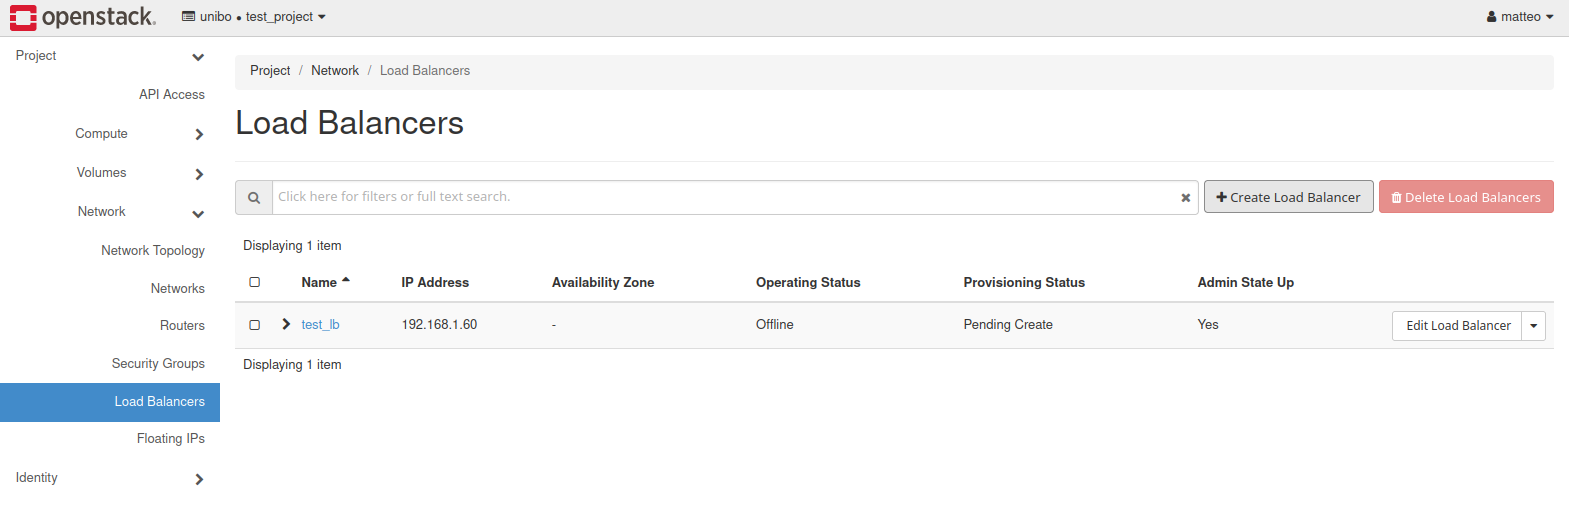
\includegraphics[scale=0.35]{tesi/files/immagini/load_balancer_usage/load_balancers_interface.png}
    \caption{Interfaccia di gestione dei load balancers}
    \label{fig:lb_mgmt_interface}
\end{figure}

Per creare un nuovo load balancer si deve cliccare il bottone \emph{Create load balancer}; in questo modo verrà aperta una finestra di dialogo che consentirà all'utente di inserire tutti i parametri di configurazione. Gli unici parametri obbligatori sono il nome e la subnet alla quale collegare l'interfaccia di rete. È possibile inoltre creare il listener e il pool direttamente da questa finestra di dialogo, però questi elementi verranno trattati nella \cref{subsec:load_balancer_management}.

\subsection{Gestione del load balancer}\label{subsec:load_balancer_management}

Cliccando sul nome di uno dei load balancer è possibile accedere alla pagina di gestione, dalla quale si possono visualizzare tutte le informazioni riguardanti il load balancer selezionato e gestire i listener e i pool.

\begin{figure}[H]
    \center
    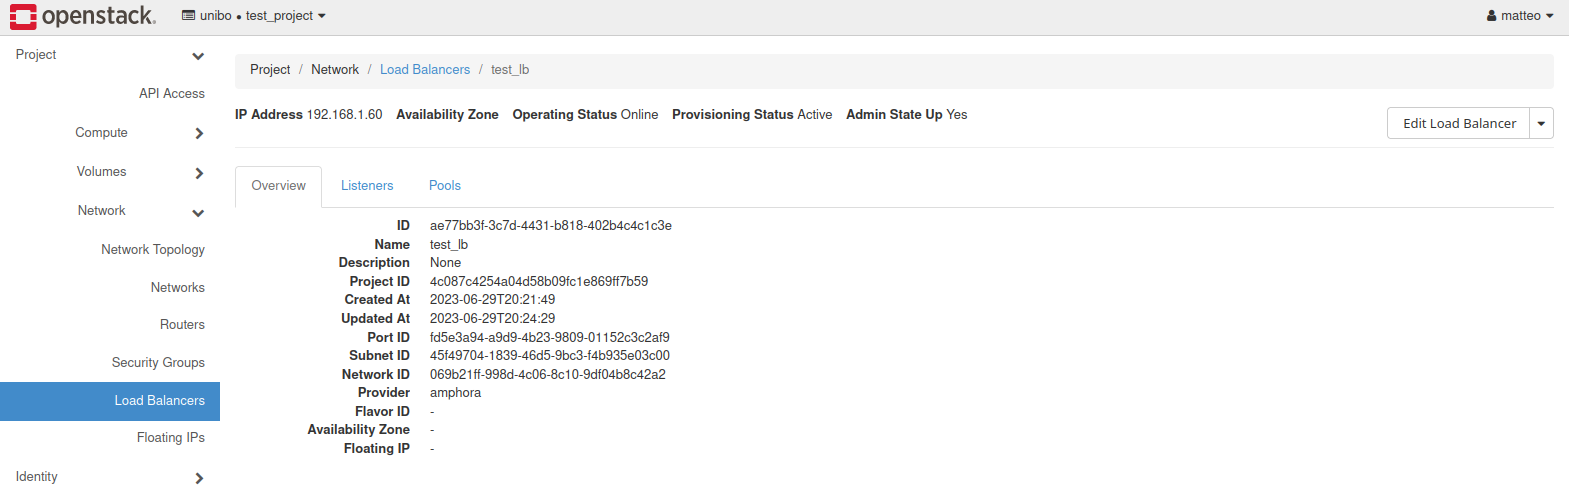
\includegraphics[scale=0.35]{tesi/files/immagini/load_balancer_usage/load_balancer_settings.png}
    \caption{Interfaccia configurazione di un load balancer}
    \label{fig:lb_settings}
\end{figure}

\paragraph{Listener.} È possibile aggiungere e modificare i listener dall'interfaccia di configurazione del load balancer andando nella scheda \emph{Listeners}. Per creare un nuovo listener si vede cliccare sul bottone \emph{Create Listener} e inserire tutti i parametri di configurazione richiesti. Nello specifico i parametri sono i seguenti:
\begin{itemize}
    \item \textbf{Name}: nome del listener
    \item \textbf{Protocol}: protocollo su cui il listener resta in ascolto
    \item \textbf{Port}: porta sulla quale il listener resta in ascolto
    \item \textbf{Client Data Timeout}: timeout del client (espresso in millisecondi)
    \item \textbf{TCP Inspect Timeout}: tempo massimo di attesa di ulteriori pacchetti TCP per l'ispezione del contenuto
    \item \textbf{Member Connect Timeout}: timeout di connessione per i membri dei pool
    \item \textbf{Member Data Timeout}: timout di inattività per i membri dei pool
    \item \textbf{Connection Limit}: numero massimo di connessioni simultanee (si può disabilitare inserendo -1)
    \item \textbf{Allowed Cidrs}: permette di restringere le connessioni solamente alle subnet specificate
\end{itemize}

È possibile inoltre creare un pool contemporaneamente al listener oppure associarene uno in seguito.

\paragraph{Pool.} Per creare e gestire i pool si deve aprire la scheda \emph{Pools} all'interno dell'interfaccia di gestione del load balancer. Da qui è possibile midificare o pool esistenti oppure crearne uno nuovo cliccando sul bottone \emph{Create Pool}. I parametri richiesti per la creazione di un nuovo pool sono:
\begin{itemize}
    \item \textbf{Name}: nome del pool
    \item \textbf{Algorithm}: algoritmo da utilizzare per il load balancing (tutti gli algoritmi sono descritti nel paragrafo seguente)
    \item \textbf{Protocol}: protocollo utilizzato dai membri del pool
    \item \textbf{Session Persistance}: permette di indicare il tipo di persistenza della sessione da utilizzare
    \item \textbf{TLS Enabled}: se attivato le connessioni tra il load balancer e i membri vengono cifrate
\end{itemize}

\paragraph{Algoritmi di load balancing.}
Il load balancer utilizzato durante lo svolgimento di questo progetto implementa 3 diversi algoritmi di load balancing:
\begin{itemize}
    \item Least Connections
    \item Round Robin
    \item Source IP
\end{itemize}

L'algoritmo \emph{Least Connections} inoltra la richiesta del client al membro del pool con il minor numero di connessioni attive al momento della richiesta. Questo può essere molto utile nel caso in cui le richieste all'applicazione ospitata dietro il load balancer abbiano tempi di risposta molto diversi (ad esempio il download di file) e nel caso in cui tutti i membri del pool abbiano risorse hardware molto simili.

L'algoritmo \emph{Round Robin} inoltra le richieste dei client a rotazione a tutti i membri del pool. Questo algoritmo può essere molto utile in casi in cui tutte le richieste sono molto simili come tempi di risposta e complessità delle operazioni da eseguire, ma potrebbe essere inefficiente nel caso in cui le richieste hanno tempi di risposta molto diversi o richiedono l'esecuzione di calcoli molto complessi.

L'algoritmo \emph{Source IP} consiste nell'indirizzare tutte le richieste provenienti dallo stesso indirizzo IP al medesimo membro del pool. Questo algoritmo è utile specialmente quando è imperativo che il client si connetta sempre allo stesso server per ciascuna richiesta.


\paragraph{Tipi di persistenza della sessione.}
Octavia implementa 3 tecniche di persistenza della sessione:
\begin{itemize}
    \item Source IP
    \item HTTP Cookie
    \item APP Cookie
\end{itemize}

Come si può intuire, se si utilizza la tecnica \emph{Source IP} la sessione viene mantenuta in base all'indirizzo IP del client. Utilizzando invece la tecnica \emph{HTTP Cookie} viene generato in automatico un cookie HTTP aggiuntivo che permette al load balancer di capire a quale membro del pool il client si è connesso in precedenza. La tecnica \emph{APP Cookie} è molto simile come funzionamento alla precedente, con l'unica differenza che il cookie non viene generato in automatico ma viene impostato dall'applicazione ospitata dietro il load balancer e, durante la configurazione del pool, deve essere specificato qual è il nome di questo cookie.


\newpage

\chapter{Introduzione}

Il cloud computing consiste in una serie di servizi che permettono di creare e gestire risorse IT on-demand con una tariffa basata sul consumo. I principali vantaggi sono la flessibilità dell'infrastruttura e la notevole riduzione dei costi di manutenzione, considerando anche che rispetto ad un'infrastruttura on-premises non c'è nessun tipo di hardware da gestire. Per questi motivi negli ultimi anni la richiesta di servizi di cloud computing è aumentata notevolmente e ad oggi di tratta di un mercato da centinaia di miliardi di dollari all'anno che vede come player principali Amazon Web Services, Google Cloud Platform e Microsoft Azure.

Purtroppo però non è tutto oro quel che luccica; esistono infatti diversi svantaggi nell'utilizzare questi tipi di servizi tra i quali il più rilevante è sicuramente il costo. Nonostante i benefici citati prima può essere poco conveniente utilizzare servizi di cloud compunting per casi d'uso in cui si ha bisogno di ingenti risorse di calcolo o di elevati volumi di storage. Per questo motivo molte realtà aziendali preferiscono creare un'infrastruttura cloud privata. Ci sono numerose piattaforme che permettono di realizzare questo tipo di infrastrutture e una di queste è OpenStack.

OpenStack è una piattaforma di cloud computing open source che permette di realizzare infrastrutture cloud sia private che pubbliche. Esistono infatti cloud provider che utilizzano OpenStack come base per erogare i loro servizi; un esempio è OVH, uno dei più grandi provider d'Europa.
OpenStack è anche scelto da molte aziende come base per il loro cloud privato per via della sua architettura modulare e grazie al fatto che le funzionalità offerte sono molto simili a quelle dei cloud provider.

\section{Il progetto}

L'obiettivo di questo progetto di tesi è prima di tutto installare e configurare un cloud privato basato su OpenStack per poi scoprirne le caratteristiche e studiarne le funzionalità nel dettaglio.

È inoltre previsto lo studio di Terraform, un Infrastructure as Code (IaC) tool, ovvero uno strumento che permette di definire infrastrutture cloud utilizzando solamente codice scritto all'interno di file di configurazione. In particolare si vuole studiare come questo strumento si integra con OpenStack e di come è possibile creare risorse all'interno di OpenStack utilizzandolo.

\section{Struttura del documento}

In questa sezione verrà esplicitata la struttura del documento descrivendo in maniera molto sintetica il contenuto di ciascun capitolo.

\begin{description}
    \item \textbf{Obiettivi} - Descrizione approfondita degli obbiettivi posti per lo svolgimento del progetto.
    \item \textbf{Progettazione del cluster} - Descrizione dell'architettura del cloud e approfondimento sulle scelte di progettazione e sulle motivazione di tali scelte.
    \item \textbf{Prerequisiti} - Descrizione dei componenti software necessari come supporto all'installazione di OpenStack (MAAS e Juju) e spiegazione delle procedure di installazione e configurazione di tali componenti.
    \item \textbf{OpenStack} - Descrizione della piattaforma OpenStack, dei suo componenti principali che verranno installati e dei software esterni necessari per far funzionare la piattaforma.
    \item \textbf{Installazione di OpenStack} - Descrizione delle procedure di installazione manuale e in bundle di OpenStack e spiegazione delle procedure di configurazione.
    \item \textbf{Utilizzo di OpenStack} - Istruzioni su come utilizzare al meglio un cloud OpenStack e su come sfruttarne a pieno le risorse.
    \item \textbf{Load Balancer} - Descrizione del servizio di load balancing di OpenStack, dei componenti che ne fanno parte, spiegazione delle procedure di installazione e di configurazione di tali componenti e istruzioni per l'utilizzo del load balancer.
    \item \textbf{Terraform} - Descrizione del tool Terraform, di come questo tool si integra con OpenStack e dei progetti Terraform realizzati durante lo svolgimento della tesi.
\end{description}


\section{Terraform e OpenStack}

\subsection{Introduzione}
Durante lo svolgimento di questo progetto io e il mio collega Sauro abbiamo deciso di prendere due direzioni diverse per quanto riguarda lo studio dell'integrazione tra Terraform e OpenStack: io ho approcciato il provisioning delle risorse tramite Terraform dal punto di vista di un utente che utilizza OpenStack come cloud provider per ospitare le proprie applicazioni, mentre il mio collega si è concentrato maggiormente sul provisioning delle risorse dal punto di vista dell'amministratore del cloud.

L'approccio che ho utilizzato per questo studio è stato iterativo: ho iniziato con un progetto molto semplice che consisteva nel creare una sola istanza per poi arrivare alla terza iterazione ad un progetto molto più complesso che utilizza tutte le possibili risorse offerte dal nostro cloud OpenStack e simula in maniera abbastanza realistica quello che potrebbe essere un caso d'uso reale. Nelle sezioni seguenti saranno descritti nel dettaglio tutti i progetti Terraform che ho realizzato.

\subsection{Progetto 1: istanza}

Come accennato in precedenza il primo progetto consiste solamente nel deployment di un'istanza tramite Terraform. L'unico file presente è \verb|main.tf| che al suo interno contiene 3 blocchi che verranno riportati e descritti di seguito.

\paragraph{Blocco terraform.}
Il primo blocco è di tipo \code{terraform}, ovvero quello che contiene le impostazioni di Terraform e la lista dei provider necessari per il deployment dell'infrastruttura.
\lstinputlisting[language=hcl,caption={Blocco di tipo \code{terraform}},label={lst:project1_terraform_block},firstline=1,lastline=9]{tesi/files/terraform_projects/01_simple/main.tf}

\paragraph{Blocco provider.}
Il secondo blocco è di tipo \code{provider} e permette di definire le informazioni di connessione ai provider scelti (in questo caso OpenStack).
\lstinputlisting[language=hcl,caption={Blocco di tipo \code{provider}},label={lst:project1_provider_block},firstline=11,lastline=18]{tesi/files/terraform_projects/01_simple/main.tf}
\noindent
Come si può vedere dal \cref{lst:project1_provider_block} il provider OpenStack accetta i seguenti parametri:
\begin{itemize}
    \item \code{user\_name}: nome dell'utente con il quale accedere alle API di OpenStack
    \item \code{password}: password dell'utente
    \item \code{auth\_url}: endpoint di Keystone, il servizio che gestisce le identità su OpenStack (per altri dettagli vedere \cref{sec:openstack_keystone})
    \item \code{domain\_name}: nome del dominio all'interno del quale è definito l'utente
    \item \code{tenant\_name}: nome del progetto all'interno del quale devono essere create le risorse definite tramite Terraform
    \item \code{insecure}: permette di specificare se autorizzare o meno le connessioni HTTPS se i certificati SSL non sono validi
\end{itemize}



\paragraph{Blocco resource.}
Il terzo e ultimo blocco è di tipo \code{resource} ed è stato utilizzato per definire i dettagli dell'istanza da creare. 
\lstinputlisting[language=hcl,caption={Blocco di tipo \code{resource}},label={lst:project1_resource_block},firstline=20,lastline=30]{tesi/files/terraform_projects/01_simple/main.tf}
\noindent
Come si può vedere dal \cref{lst:project1_resource_block} il tipo di risorsa da utilizzare per creare un'istanza è \code{openstack\_compute\_instance\_v2} e, in questo caso, il nome assegnato alla risorsa è \code{test-server}. Gli argomenti per configurare l'istanza sono gli stessi trattati nella \cref{sec:openstack_usage_instances} quando si parla dell'interfaccia che permette di creare una nuova istanza.

Come si può notare sempre dal \cref{lst:project1_resource_block} la configurazione della rete è definita tramite blocchi all'interno della risorsa; in questo caso il blocco è molto semplice perché viene specificato solo il nome della rete a cui l'istanza deve essere collegata.

\paragraph{Deployment dell'infratruttura}

Lanciando il comando il comando \verb|terraform apply| partendo da un progetto senza nessuna risorsa già creata si ottiene l'output mostrato in \cref{fig:terraform_project1_apply} (ritagliato per motivi di spazio). Come si può notare Terraform mostra tutte le modifiche che intende fare all'infrastruttura e chiede conferma all'utente prima di eseguire qualsiasi azione. Una volta data la conferma Terraform procederà con la creazione delle risorse mostrate e attenderà fino a quando ciascuna di esse sarà attiva.
\begin{figure}[H]
    \center
    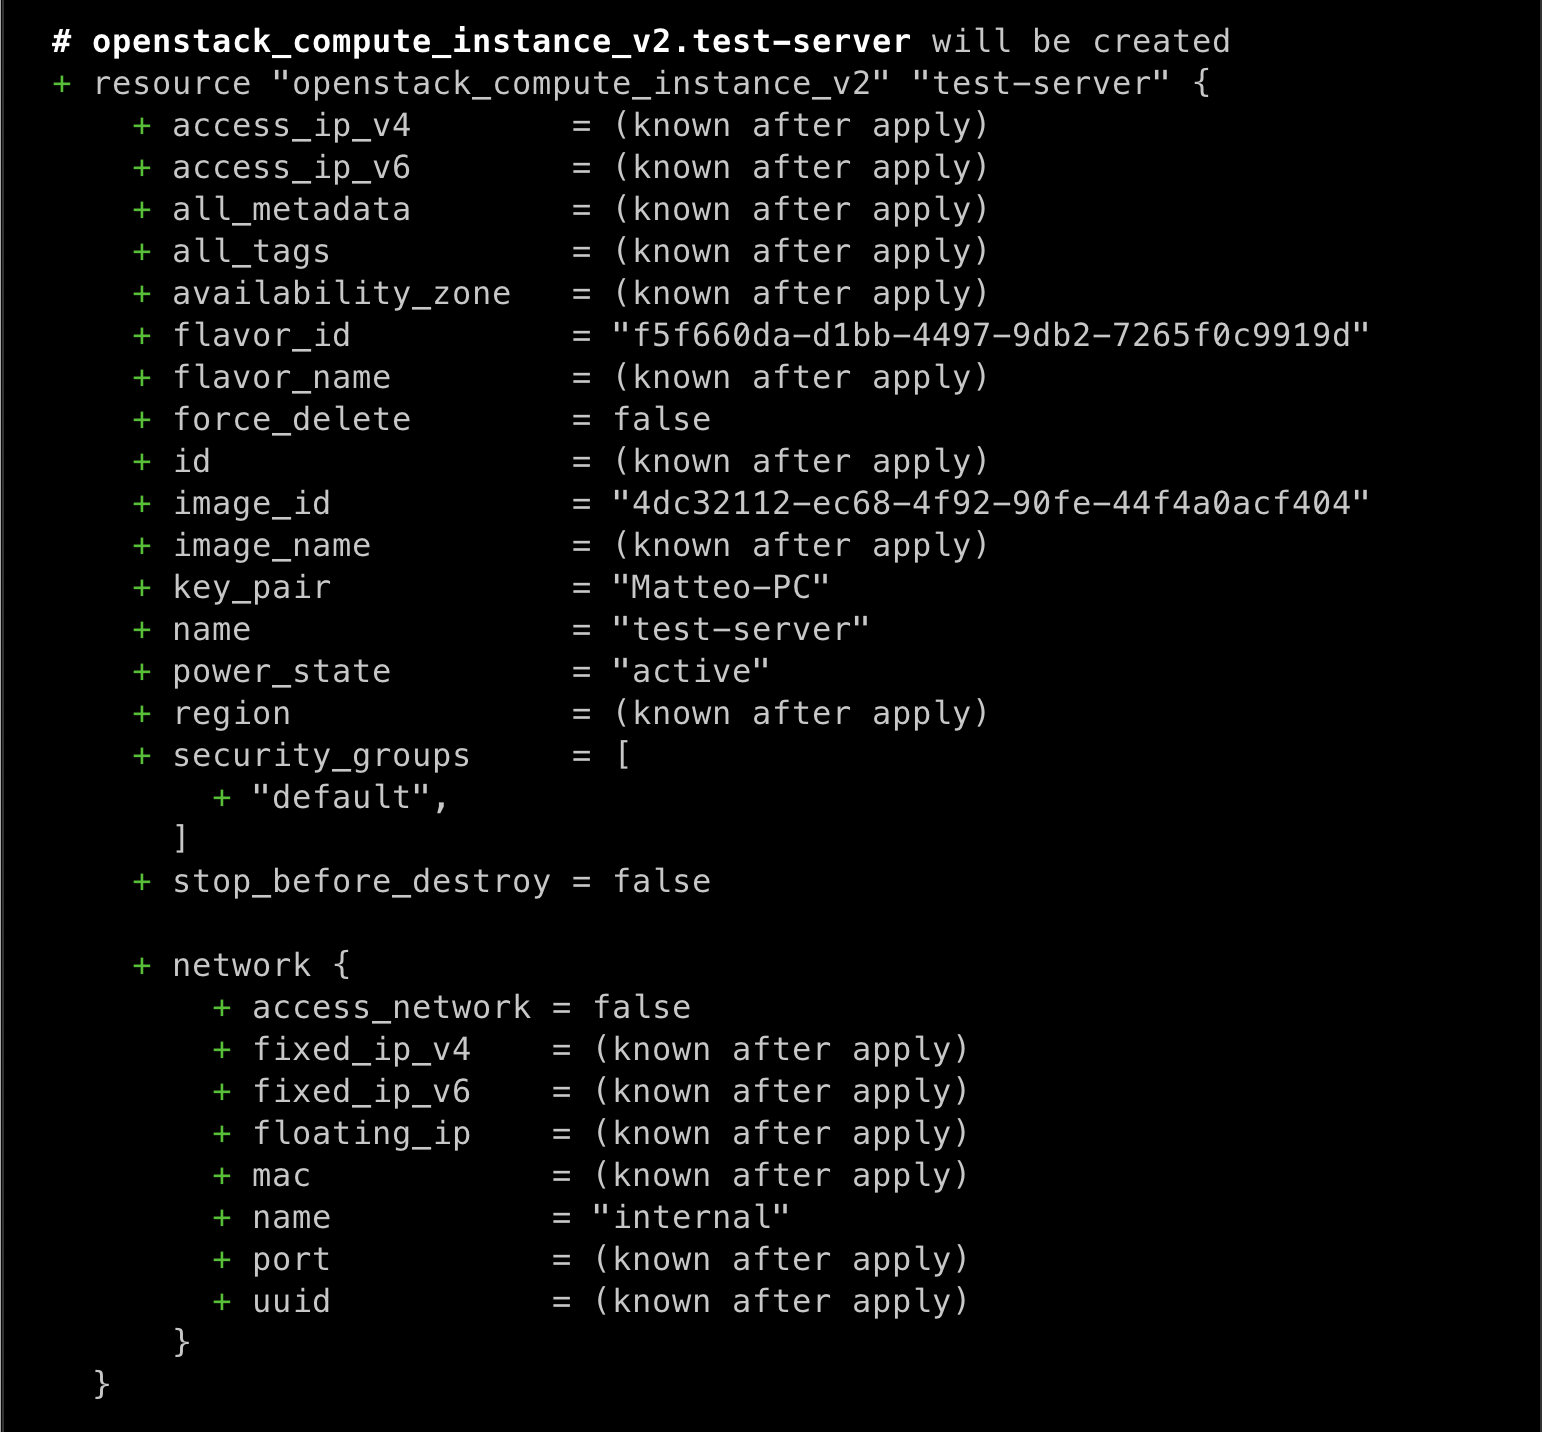
\includegraphics[scale=0.35]{tesi/files/immagini/terraform/projects/project1_terraform_apply.png}
    \caption{Pianificazione delle modifiche all'infrastruttura}
    \label{fig:terraform_project1_apply}
\end{figure}

\subsection{Progetto 2: infrastruttura completa}

Il secondo progetto sviluppato è ovviamente un'evoluzione del primo e prevede la configurazione tramite Terraform di un'infrastruttura completa. Per infrastruttura completa si intende che la configurazione deve includere sia le istanze che tutta la parte di networking.

In questo caso la struttura del progetto rimane abbastanza semplice ma sono stati aggiunti alcuni file in modo mantenere tutto il codice più organizzato. Di seguito è riportato uno schema della struttura del progetto:
\dirtree{%
.1 02\_full\_infrastructure.
.2 example.tfvars.
.2 instances.tf.
.2 main.tf.
.2 networking.tf.
}

In \cref{app:tf_proj2} è possibile vedere tutti i file di questo progetto compresi quelli che non vengono mostrati qui per motivi di spazio.

\paragraph{Variabili di input.} All'interno di questo progetto sono state aggiunte alcune variabili di input. Queste variabili sono dichiarate all'interno del file \verb|main.tf| nel seguente modo:
\lstinputlisting[language=hcl,caption={},firstline=12,lastline=45]{tesi/files/terraform_projects/02_full_infrastructure/main.tf}
\noindent
Come si può notare ciascuna variabile dichiarata è di tipo \code{object} e al suo interno contiene altre variabili di tipi differenti. Quando si esegue il deployment tramite Terraform è necessario specificare un file tramite l'argomento \verb|-varfile| che contiene le assegnazioni dei valori a queste variabili. All'interno del progetto è presente infatti il file \verb|example.tfvars| che contiene appunto un esempio di come deve essere strutturato un file con tutte le variabili di questo progetto assegnate.
\lstinputlisting[language=hcl,caption={}]{tesi/files/terraform_projects/02_full_infrastructure/example.tfvars}
La sintassi generica per poter accedere alle variabili definite all'interno del progetto è la seguente: \code{var.<nome\_variabile>}; dato che le variabili definite qui contengono a loro volta altre variabili per accedere ad esempio al nome dell'utente la sintassi è la seguente: \code{var.auth.user}.

\paragraph{Networking.} Tutte le configurazioni riguardanti la rete dell'infrastruttura si trovano nel file \verb|networking.tf|. Al suo interno ci sono 5 blocchi di tipo \code{resource} utilizzati per configurare le seguenti risorse:
\begin{itemize}
    \item network
    \item subnet
    \item security group da assegnare all'istanza
    \item router
    \item interfaccia che collega il router alla subnet definita in precedenza
\end{itemize}

Nel \cref{lst:project2_router_interface} è riportato il blocco che configura il collegamento del router alla subnet tramite una nuova interfaccia.
\lstinputlisting[language=hcl,label={lst:project2_router_interface},caption={Configurazione dell'interfaccia del router che lo collega alla subnet},firstline=33,lastline=36]{tesi/files/terraform_projects/02_full_infrastructure/networking.tf}
\noindent
Come si può notare gli unici due argomenti sono l'ID del router e l'ID della subnet a cui l'interfaccia si deve collegare. Questo esempio è interessante perché mostra come è possibile utilizzare gli argomenti di determinate risorse per configurarne altre. Nello specifico la sintassi utilizzata per accedere agli argomenti di altre risorse è la seguente: \code{<tipo\_risorsa>.<etichetta\_risorsa>.<parametro>}. Se ad esempio si volesse accedere all'argomento \code{router\_id} dell'interfaccia creata dall'esempio sopra la sintassi sarebbe la seguente: \\
\code{openstack\_networking\_router\_interface\_v2.tf\_router\_interface.router\_id}.

\paragraph{Istanza}

Tutte le configurazioni riguardanti l'istanza si trovano all'interno del file \verb|instances.tf|. Il blocco riguardante l'istanza stessa è molto simile a quello del progetto precedente con una sola eccezione: in questo caso è stato aggiunto un altro blocco al suo interno chiamato \code{block\_device} (riportato nel \cref{lst:project2_block_device}) che permette di collegare un volume all'istanza.
\lstinputlisting[
    language=hcl,
    label={lst:project2_block_device},
    caption={Configurazione di un volume collegato all'istanza},
    firstline=7,
    lastline=14
]{tesi/files/terraform_projects/02_full_infrastructure/instances.tf}

All'interno del file \verb|instances.tf| è anche presente la configurazione del floating IP e l'assegnazione di quest'ultimo all'istanza creata.


\subsection{Progetto 3: Proof of Concept}

Il terzo progetto è l'ultima iterazione e sfrutta tutte le funzionalità offerte dal cloud OpenStack installato. Lo scopo è quello di simulare il deployment di un'applicazione web reale creando più istanze e configurando un load balancer in modo che divida le richieste tra di esse. In \cref{fig:terraform_project3_network_topology} è raffigurata la topologia di rete (escluso il load balancer); come si può vedere sono presenti 3 istanze collegate ad una rete privata alla quale è collegato anche un router che permette alle suddette istanze di accedere a internet. Il load balancer è configurato in modo da essere collegato sia alla rete pubblica che a quella privata così da poter essere raggiungibile dai client e potersi collegare alle istanze tramite la rete interna.

\begin{figure}[H]
    \center
    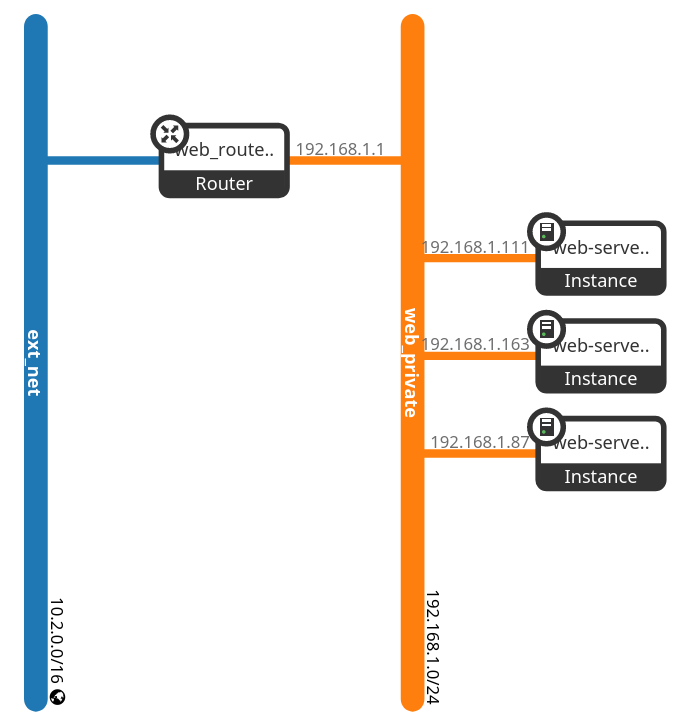
\includegraphics[scale=0.5]{tesi/files/immagini/terraform/projects/project3_network_diagram.png}
    \caption{Topologia di rete del progetto}
    \label{fig:terraform_project3_network_topology}
\end{figure}

Il progetto ha la seguente struttura:
\dirtree{%
.1 03\_proof\_of\_concept.
.2 example.tfvars.
.2 init-instance.sh.
.2 instances.tf.
.2 load\_balancer.tf.
.2 main.tf.
.2 networking.tf.
.2 output.tf.
}
\noindent
Tutti i file del progetto compresi quelli non riportati in questa sezione possono essere consultati in \cref{app:tf_proj3}

\paragraph{Istanze.}

La configurazione delle istanze si trova all'interno del file \\
\verb|instances.tf| che, rispetto al progetto precedente, presente 2 aggiunte: l'argomento \code{count} che permette di specificare il numero di istanze da creare e il parametro \code{user\_data} che permette di specificare uno script bash che sarà poi eseguito dalle macchine all'avvio. La porzione di configurazione dell'argomento \code{user\_data} è la seguente:
\lstinputlisting[language=hcl,caption={},firstline=10,lastline=12]{tesi/files/terraform_projects/03_proof_of_concept/instances.tf}
\noindent
In questo caso viene utilizzata la funzione \code{templatefile} per caricare uno script da file e nello specifico carica il file chiamato \verb|init-instance.sh| contenuto nella directory principale del modulo; il secondo argomento di tale funzione è un oggetto che permette di inoltrare variabili allo script (in questo caso \code{instance\_idx}. Lo script \verb|init-instance.sh| è molto semplice ed è riportato di seguito:
\lstinputlisting[language=mybash,caption={}]{tesi/files/terraform_projects/03_proof_of_concept/init-instance.sh}
\noindent
Il suo compito è quello di installare Apache Web Server e di creare un file \verb|index.html| all'interno del quale viene scritto l'indice della macchina appena creata. In questo modo ciascuna macchina creata avrà un indice diverso e, accedendo attraverso il load balancer, sarà possibile capire a quale macchina ci si sta connettendo e verificare che l'algoritmo di load balancing stia funzionando come ci si aspetta.

\paragraph{Load Balancer.}

Tutte le configurazione del load balancer si trovano all'interno del file \verb|load_balancer.tf|. Di seguito è riportata la configurazione del pool che potrebbe essere interessante perché contiene un blocco dinamico:
\lstinputlisting[language=hcl,caption={},firstline=7,lastline=29]{tesi/files/terraform_projects/03_proof_of_concept/load_balancer.tf}
\noindent
Il primo blocco di questa configurazione è quello che definisce il pool; si può notare come l'algoritmo utilizzato per il load balancing è round robin e che il protocollo specificato per la connessione agli host è HTTP. Il secondo blocco invece è la configurazione dei membri del pool; al suo interno si trova un altro blocco dinamico chiamato \code{"member"} che itera le istanze creando per ciascuna un blocco contenente come argomenti l'indirizzo IP, la porta su cui è esposto il servizio e il peso (utilizzato durante il load balancing per dare priorità di connessione ad una macchine rispetto alle altre).

Sono inoltre configurati un listener sulla porta 80 con protocollo HTTP e un health monitor che esegue periodicamente richieste HTTP alle istanze per verificare che siano ancora online e che il web server stia funzionando correttamente.

\paragraph{Output.}

Terraform permette di definire un output che viene generato una volta completate le modifiche e permette di visualizzare alcune informazioni potenzialmente molto utili sull'infrastruttura appena creata. All'interno del file \verb|output.tf| sono presenti due blocchi di tipo output:
\lstinputlisting[language=hcl,caption={}]{tesi/files/terraform_projects/03_proof_of_concept/outputs.tf}
\noindent
Il primo blocco mostra il floating IP assegnato al load balancer mentre il secondo mostra i dettagli di tutte le istanze create. In \cref{fig:terraform_project3_output} è mostrato un esempio di quello che viene scritto in output dichiarando questi due blocchi.

\begin{figure}[H]
    \center
    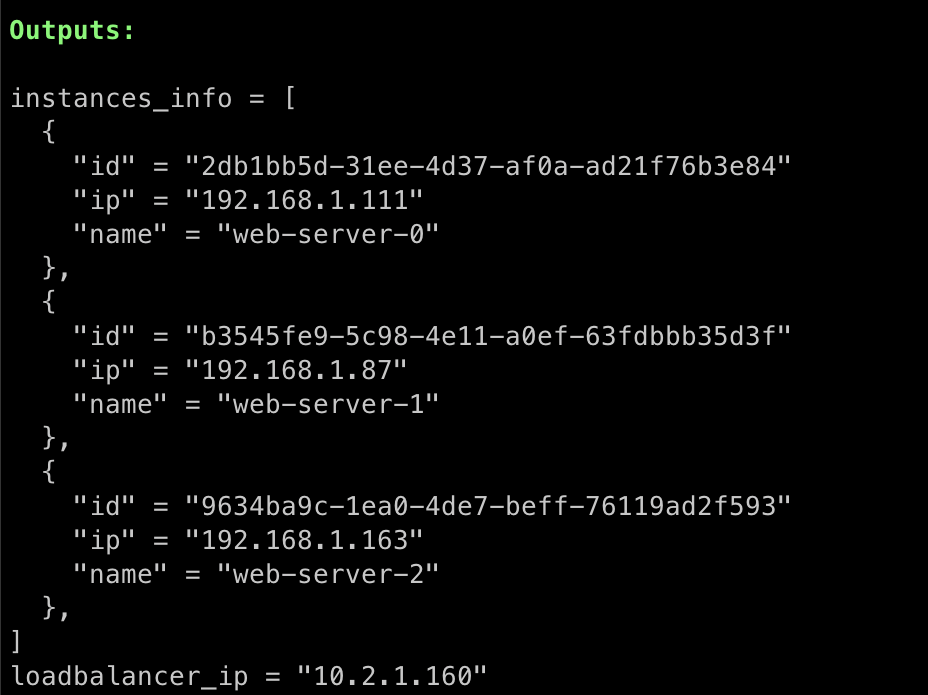
\includegraphics[scale=0.6]{tesi/files/immagini/terraform/projects/project3_output.png}
    \caption{Output di terraform}
    \label{fig:terraform_project3_output}
\end{figure}


\newpage

\chapter{Conclusioni e sviluppi futuri}

Si può affermare di aver ampiamente raggiunto gli obbiettivi posti all'inizio del progetto, riuscendo a realizzare un cloud privato funzionante basato su OpenStack e a realizzare infrastrutture appoggiate a tale cloud utilizzando esclusivamente Terraform.

\paragraph{OpenStack.} OpenStack si è rivelato essere una piattaforma estremamente versatile e personalizzabile, adatta a molteplici esigenze e casi d'uso grazie alla sua modularità e alle funzionalità che offre. OpenStack offre infatti un set di funzionalità paragonabile ad un qualsiasi cloud provider e, in base alla mia esperienza, addirittura superiore ad altri sistemi esistenti che permettono di realizzare cloud privati, sia a pagamento che open source (ad esempio VMware vSphere o Proxmox).

L'unica criticità che ho riscontrato in OpenStack è legata al numero di servizi richiesti per far funzionare il cloud; sono infatti presenti numerosi servizi che definirei di "supporto", ovvero che servono per far funzionare la piattaforma ma non aggiungono alcun tipo di funzionalità per l'utente finale. Questi servizi causano un overhead di risorse che, nel caso di deployment di piccole dimensioni e con poche risorse hardware disponibili, potrebbe essere critico o addirittura determinate l'esclusione di OpenStack dalla lista delle possibili piattaforme su cui basare il cloud.

\paragraph{Deployment del cloud.} I sistemi di supporto al deployment utilizzati (MAAS e Juju) hanno notevolmente facilitato l'installazione e la configurazione, creando un livello di astrazione aggiuntivo tra l'utente e i singoli servizi. È bastato infatti scrivere poche linee di configurazione per installare tutto il cloud senza la necessità intervenire sui singoli file di configurazione di ciascun servizio.

Questa ulteriore astrazione porta però con sé una criticità: è molto complicato e addirittura sconsigliato da Juju andare a modificare manualmente i file di configurazione dei singoli servizi; questo può essere un problema specialmente nei casi in cui si tratta di servizi distribuiti su più macchine, come ad esempio Ceph o Nova.

Nel caso di Ceph per esempio, è necessario che tutte le macchine abbiano esattamente lo stesso numero di dischi configurati nello stesso modo perché, come visto nella \cref{sec:openstack_manual_installation}, i device assegnati a Ceph vengono definiti globalmente e non possono essere modificati per una singola macchina.

Questa limitazione nella configurazione porta ad avere la necessità di installare tutti i servizi dello stesso tipo su macchine molto simili se non identiche.

\paragraph{Terraform.} Personalmente prima dell'inizio di questo progetto di tesi non conoscevo tool come Terraform o simili; nonostante questo è stato relativamente semplice utilizzarlo grazie anche alla documentazione molto esaustiva fornita. Terraform si è rivelato essere uno strumento estremamente potente e utile, che permette realizzare e modificare infrastrutture molto complesse in maniera abbastanza semplice e sicuramente più veloce rispetto ad eseguire tutte le operazioni manualmente.

\section{Sviluppi futuri}

La prima attività da menzionare quando si parla dei possibili sviluppi futuri è sicuramente verificare che la metodologia di deployment utilizzata durante questo progetto sia ancora valida per le versioni successive di OpenStack. Dato il livello di astrazione fornito dai sistemi di deployment utilizzati mi sento abbastanza sicuro nel dire che dovrebbe bastare la modifica di alcuni parametri all'interno dei file bundle di Juju per poterli riutilizzare per il deployment di una versione successiva.

Un'altra attività fondamentale sarebbe quella di verificare lo stato dei dischi all'interno delle macchine e, nel caso siano danneggiati, sostituirli e rifare il deployment del cloud. Questo perché durante lo svolgimento del progetto sono sorti alcuni problemi di responsività del sistema e, dato il fallimento del test S.M.A.R.T. su alcune macchine, si presume che alcuni dischi abbiano dei settori danneggiati e che ciò influisca in maniera negativa sulle performance.

Altre possibili attività potrebbero riguardare l'installazione e la configurazione di servizi aggiuntivi di OpenStack, come ad esempio Zun che permette di gestire container direttamente da OpenStack senza dover creare istanze, oppure Trove che implementa un servizio di database as a service. Mi sembra chiaro ormai che se si vogliono esplorare altri componenti e funzionalità di OpenStack le possibilità sono moltissime e c'è l'imbarazzo della scelta.

\clearpage


%bibliografia
\bibliographystyle{splncs04}
{
    \raggedright
    \bibliography{tesi/testo/20_reference.bib}
}
\clearpage

%appendice
\appendix
%\chapter{Listati dei comandi}

%\section{Installazione di MAAS}\label{sec:appendice_maas}

%Di seguito sono riportati i comandi per l'installazione completa di MAAS.

%\lstinputlisting[
%caption={Installazione di MAAS.},
%    language=appendice,
%]
%{tesi/files/installazioni/CLI/maas.txt}



%\section{Installazione di Juju}\label{sec:appendice_juju}

%Di seguito sono riportati i comandi per la corretta installazione di Juju e dell'inizializzazione del cloud.

%\lstinputlisting[
%caption={Installazione di Juju e inizializzazione del cloud.},
%    language=appendice,
%]
%{tesi/files/installazioni/CLI/juju.txt}



%\section{Installazione semi-automatizzata di OpenStack}\label{sec:appendice_openstack}
%Di seguito è riportato l'elenco completo dei comandi eseguiti per il deploy di OpenStack attraverso Juju.
% 
%In rosso sono evidenziati quei valori che necessitano di essere modificati.
%\lstinputlisting[
%caption={Installazione di OpenStack attraverso Juju.},
%    language=appendice,
%]
%{tesi/files/installazioni/CLI/openstack.txt}

\chapter{Bundle di installazione}
In questo capitolo verranno riportate le versioni finali del bundle di installazione di OpenStack e del bundle overlay che permette di installare Octavia e Barbican.

\section{OpenStack}\label{app:openstack_bundle}

\lstinputlisting[language=yaml,caption={}]{tesi/files/bundles/main.yaml}

\section{Octavia e Brabican}\label{app:barbican_octavia_overlay}

\lstinputlisting[language=yaml,caption={}]{tesi/files/bundles/octavia.yaml}

\chapter{Progetti Terraform}

\section{Progetto 1: istanza}\label{app:tf_proj1}

\subsection{main.tf}
\lstinputlisting[language=hcl,caption={}]{tesi/files/terraform_projects/01_simple/main.tf}

\section{Progetto 2: infrastruttura completa}\label{app:tf_proj2}

\subsection{example.tfvars}
\lstinputlisting[language=hcl,caption={}]{tesi/files/terraform_projects/02_full_infrastructure/example.tfvars}
\subsection{instances.tf}
\lstinputlisting[language=hcl,caption={}]{tesi/files/terraform_projects/02_full_infrastructure/instances.tf}
\subsection{main.tf}
\lstinputlisting[language=hcl,caption={}]{tesi/files/terraform_projects/02_full_infrastructure/main.tf}
\subsection{networking.tf}
\lstinputlisting[language=hcl,caption={}]{tesi/files/terraform_projects/02_full_infrastructure/networking.tf}

\section{Progetto 3: Proof of Concept}\label{app:tf_proj3}

\subsection{example.tfvars}
\lstinputlisting[language=hcl,caption={}]{tesi/files/terraform_projects/03_proof_of_concept/example.tfvars}
\subsection{init-instance.sh}
\lstinputlisting[language=hcl,caption={}]{tesi/files/terraform_projects/03_proof_of_concept/init-instance.sh}
\subsection{instances.tf}
\lstinputlisting[language=hcl,caption={}]{tesi/files/terraform_projects/03_proof_of_concept/instances.tf}
\subsection{load\_balancer.tf}
\lstinputlisting[language=hcl,caption={}]{tesi/files/terraform_projects/03_proof_of_concept/load_balancer.tf}
\subsection{main.tf}
\lstinputlisting[language=hcl,caption={}]{tesi/files/terraform_projects/03_proof_of_concept/main.tf}
\subsection{networking.tf}
\lstinputlisting[language=hcl,caption={}]{tesi/files/terraform_projects/03_proof_of_concept/networking.tf}
\subsection{outputs.tf}
\lstinputlisting[language=hcl,caption={}]{tesi/files/terraform_projects/03_proof_of_concept/outputs.tf}

